% Multinational Firms and Trade in Latin America -- WP_total (reference document: all goods)
% Overleaf project exported 2026-09-24 from the build of 2026-09-23 (stylized_facts/python/wp_export_overleaf.py).
% Compile with pdfLaTeX, the Overleaf default. Figures are in figures/<scope>/ and tables in tables/<scope>/,
% where <scope> is the sample: all = all goods; agro, manufacturing, mining, rest = the sectors;
% sectors = exhibits that compare the sectors. Each figure and table below starts with a '% ----' line.
\documentclass[11pt,a4paper]{article}
\usepackage[utf8]{inputenc}
\usepackage[T1]{fontenc}
\usepackage{mathptmx}
\usepackage[margin=2.2cm]{geometry}
\usepackage{graphicx,booktabs,amsmath,amssymb,adjustbox,float,caption,hyperref,xcolor,enumitem}
\captionsetup{font=small,labelfont=bf,skip=4pt}
\hypersetup{colorlinks,linkcolor=blue!50!black,urlcolor=blue!50!black}
\setlength{\parskip}{4pt}
\title{Multinational Firms and Trade in Latin America\\[4pt]\large Stylized Facts: All Tables and Figures, All Goods}
\author{Ignacio Marra de Arti\~nano \and Gabriel Scattolo \and Sebasti\'an Vel\'asquez \and Christian Volpe Martincus}
\date{September 2026}
\begin{document}
\maketitle
\tableofcontents
\clearpage

\section*{Data}
\addcontentsline{toc}{section}{Data}

The data are the customs export records of nine Latin American countries at the firm, destination,
HS6 product and year level, matched to the ownership records of Orbis and Dun \& Bradstreet. The
years covered are Argentina 2011--2019, Chile 2009--2022, Colombia 2010--2021, Costa Rica
2010--2019, the Dominican Republic 2012--2019, El Salvador 2006--2018, Paraguay 2012--2020, Peru
2010--2019 and Uruguay 2010--2019.

An exporter found in Orbis or Dun \& Bradstreet is a multinational affiliate (MNE). It is a
\emph{domestic} MNE when its ultimate parent is located in the exporting country and a
\emph{foreign} MNE otherwise; matched exporters without a recorded parent country (7.5 percent of
foreign-MNE export value) are counted as foreign. Exporters not found in either database are
\emph{local} firms. Sectors are defined on HS chapters: agriculture 01--24, mining and fuels
25--27 and 71, manufacturing 28--97 excluding 71.

\section{Fact 1: Multinationals Account for a Large Share of Exports}\label{sec:f1_all}
% ---- Figure: Multinational Share of Export Value, by Exporting Country
\begin{figure}[H]\centering%
  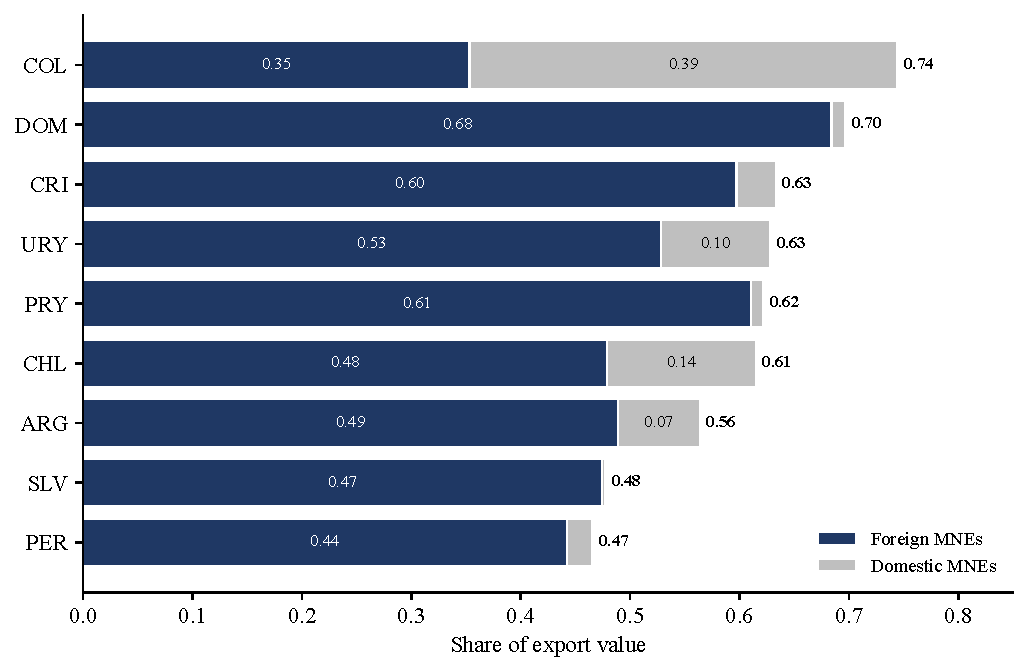
\includegraphics[width=0.8\textwidth,height=0.8\textheight,keepaspectratio]{figures/all/fig_wp0_fig1_origin.pdf}%
  \caption{Multinational Share of Export Value, by Exporting Country}%
  \label{fig:f1_all}%
  \par\vspace{2pt}%
  \parbox{0.92\textwidth}{\footnotesize %
  \textit{Notes:} Shares of export value, all available years pooled. The figure at the end of each bar is the total MNE share.\\[3pt]%
  \textit{Source:} Authors' calculations based on customs data matched to Orbis and Dun \& Bradstreet.}%
  \end{figure}
% ---- Table: Multinational Share of Export Value, by Exporting Country
\begin{table}[H]\centering\small%
  \caption{Multinational Share of Export Value, by Exporting Country}%
  \label{tab:f1n_all}%
  \adjustbox{max width=\textwidth, max totalheight=0.8\textheight}{\begin{tabular}{lrrrr}
\toprule
Origin & Foreign & Domestic & All MNEs & Value (US\$bn/yr) \\
\midrule
COL & 0.353 & 0.391 & 0.744 & 44.0 \\
DOM & 0.684 & 0.013 & 0.697 & 8.6 \\
CRI & 0.597 & 0.036 & 0.633 & 10.5 \\
URY & 0.528 & 0.100 & 0.628 & 7.0 \\
PRY & 0.611 & 0.011 & 0.622 & 7.3 \\
CHL & 0.479 & 0.136 & 0.615 & 34.2 \\
ARG & 0.489 & 0.075 & 0.564 & 66.4 \\
SLV & 0.474 & 0.003 & 0.477 & 5.0 \\
PER & 0.442 & 0.023 & 0.466 & 41.4 \\
\midrule
All & 0.463 & 0.141 & 0.605 & 224.5 \\
\bottomrule
\end{tabular}
}%
  \par\vspace{3pt}%
  \begin{minipage}{0.95\textwidth}\footnotesize %
  \textit{Notes:} Shares of export value, all available years pooled. Values are annual averages in US\$ billion.\\[3pt]%
  \textit{Source:} Authors' calculations based on customs data matched to Orbis and Dun \& Bradstreet.%
  \end{minipage}%
  \end{table}

\subsection{By Parent Country}
% ---- Figure: Multinational Share of Export Value, by Exporting Country and Parent Country
\begin{figure}[H]\centering%
  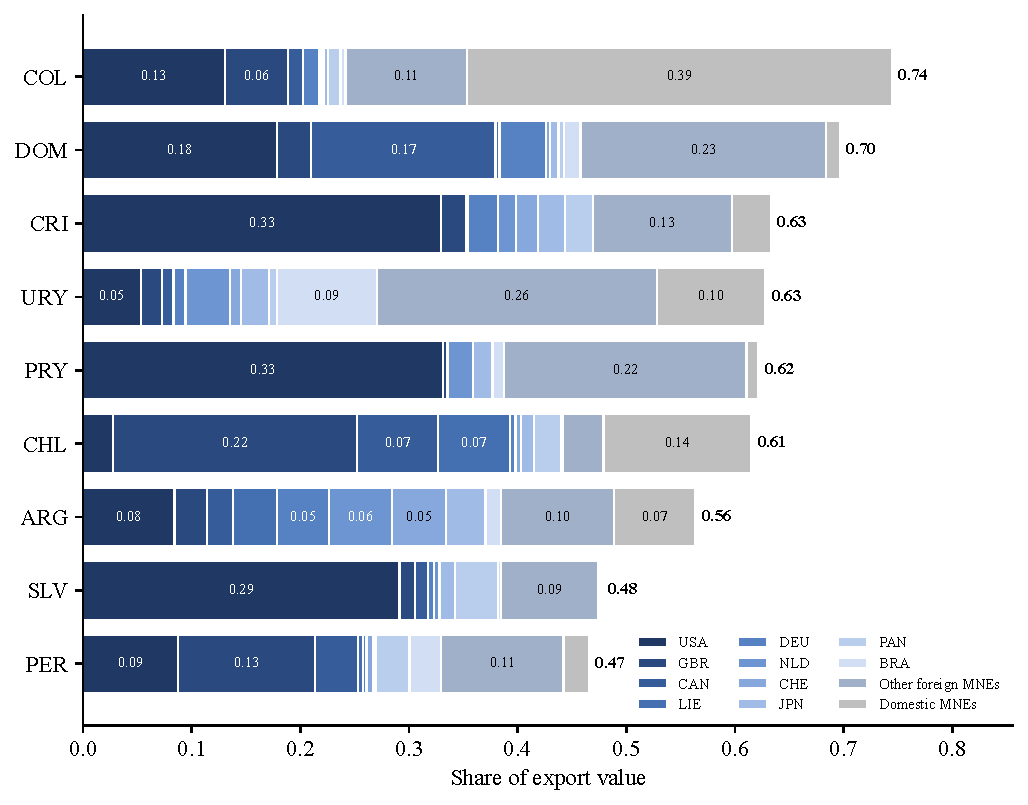
\includegraphics[width=0.92\textwidth,height=0.8\textheight,keepaspectratio]{figures/all/fig_wp1a_origin_by_parent.pdf}%
  \caption{Multinational Share of Export Value, by Exporting Country and Parent Country}%
  \label{fig:f1p_all}%
  \par\vspace{2pt}%
  \parbox{0.92\textwidth}{\footnotesize %
  \textit{Notes:} Shares of export value, all available years pooled. Foreign MNEs split by country of the ultimate parent; the ten largest parent countries are shown separately.\\[3pt]%
  \textit{Source:} Authors' calculations based on customs data matched to Orbis and Dun \& Bradstreet.}%
  \end{figure}
% ---- Table: Multinational Share of Export Value, by Exporting Country and Parent Country
\begin{table}[H]\centering\small%
  \caption{Multinational Share of Export Value, by Exporting Country and Parent Country}%
  \label{tab:f1pn_all}%
  \adjustbox{max width=\textwidth, max totalheight=0.8\textheight}{\begin{tabular}{lcccccccccccccc}
\toprule
Origin & USA & GBR & CAN & LIE & DEU & NLD & CHE & JPN & PAN & BRA & Other & Domestic & All MNEs & Value (US\$bn/yr) \\
\midrule
COL & 0.131 & 0.058 & 0.013 & 0.000 & 0.015 & 0.002 & 0.002 & 0.004 & 0.011 & 0.005 & 0.112 & 0.391 & 0.744 & 44.0 \\
DOM & 0.178 & 0.032 & 0.170 & 0.004 & 0.043 & 0.000 & 0.004 & 0.007 & 0.005 & 0.015 & 0.226 & 0.013 & 0.697 & 8.6 \\
CRI & 0.330 & 0.023 & 0.002 & 0.000 & 0.027 & 0.016 & 0.020 & 0.025 & 0.025 & 0.000 & 0.128 & 0.036 & 0.633 & 10.5 \\
URY & 0.053 & 0.020 & 0.010 & 0.000 & 0.011 & 0.041 & 0.010 & 0.026 & 0.008 & 0.091 & 0.258 & 0.100 & 0.628 & 7.0 \\
PRY & 0.331 & 0.004 & 0.000 & 0.000 & 0.000 & 0.023 & 0.000 & 0.017 & 0.001 & 0.010 & 0.223 & 0.011 & 0.622 & 7.3 \\
CHL & 0.028 & 0.225 & 0.074 & 0.066 & 0.005 & 0.000 & 0.005 & 0.012 & 0.025 & 0.001 & 0.037 & 0.136 & 0.615 & 34.2 \\
ARG & 0.084 & 0.030 & 0.024 & 0.041 & 0.047 & 0.058 & 0.050 & 0.036 & 0.001 & 0.014 & 0.104 & 0.075 & 0.564 & 66.4 \\
SLV & 0.291 & 0.015 & 0.012 & 0.000 & 0.006 & 0.005 & 0.000 & 0.014 & 0.040 & 0.003 & 0.090 & 0.003 & 0.477 & 5.0 \\
PER & 0.088 & 0.126 & 0.040 & 0.005 & 0.003 & 0.001 & 0.006 & 0.002 & 0.031 & 0.029 & 0.113 & 0.023 & 0.466 & 41.4 \\
\bottomrule
\end{tabular}
}%
  \par\vspace{3pt}%
  \begin{minipage}{0.95\textwidth}\footnotesize %
  \textit{Notes:} Shares of export value, all available years pooled. Other: all remaining foreign parents. Values are annual averages in US\$ billion.\\[3pt]%
  \textit{Source:} Authors' calculations based on customs data matched to Orbis and Dun \& Bradstreet.%
  \end{minipage}%
  \end{table}
% ---- Figure: Export Value by Exporting Country and Parent Country
\begin{figure}[H]\centering%
  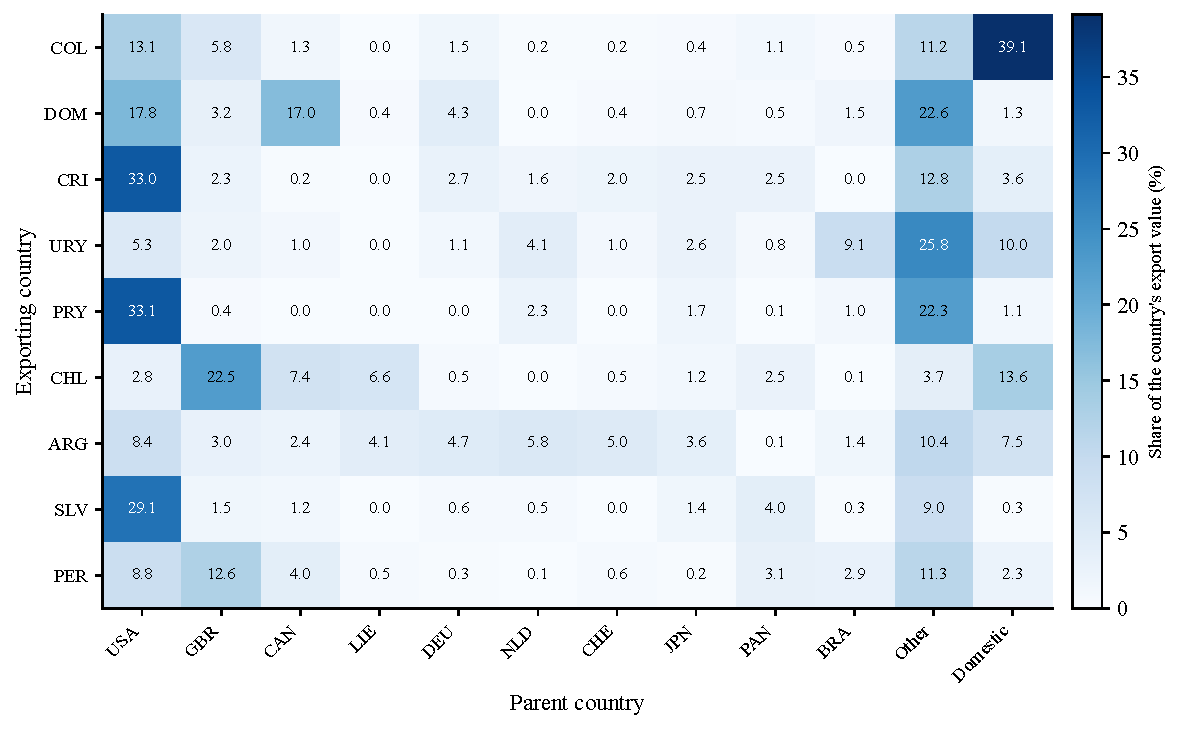
\includegraphics[width=0.9\textwidth,height=0.8\textheight,keepaspectratio]{figures/all/fig_wp1a_origin_x_parent_heatmap.pdf}%
  \caption{Export Value by Exporting Country and Parent Country}%
  \label{fig:f1hm_all}%
  \par\vspace{2pt}%
  \parbox{0.92\textwidth}{\footnotesize %
  \textit{Notes:} Percent of each country's export value, by country of the ultimate parent of the exporter.\\[3pt]%
  \textit{Source:} Authors' calculations based on customs data matched to Orbis and Dun \& Bradstreet.}%
  \end{figure}

\subsection{The United States}
% ---- Figure: Exports by US-Parent Multinationals, by Exporting Country and Sector
\begin{figure}[H]\centering%
  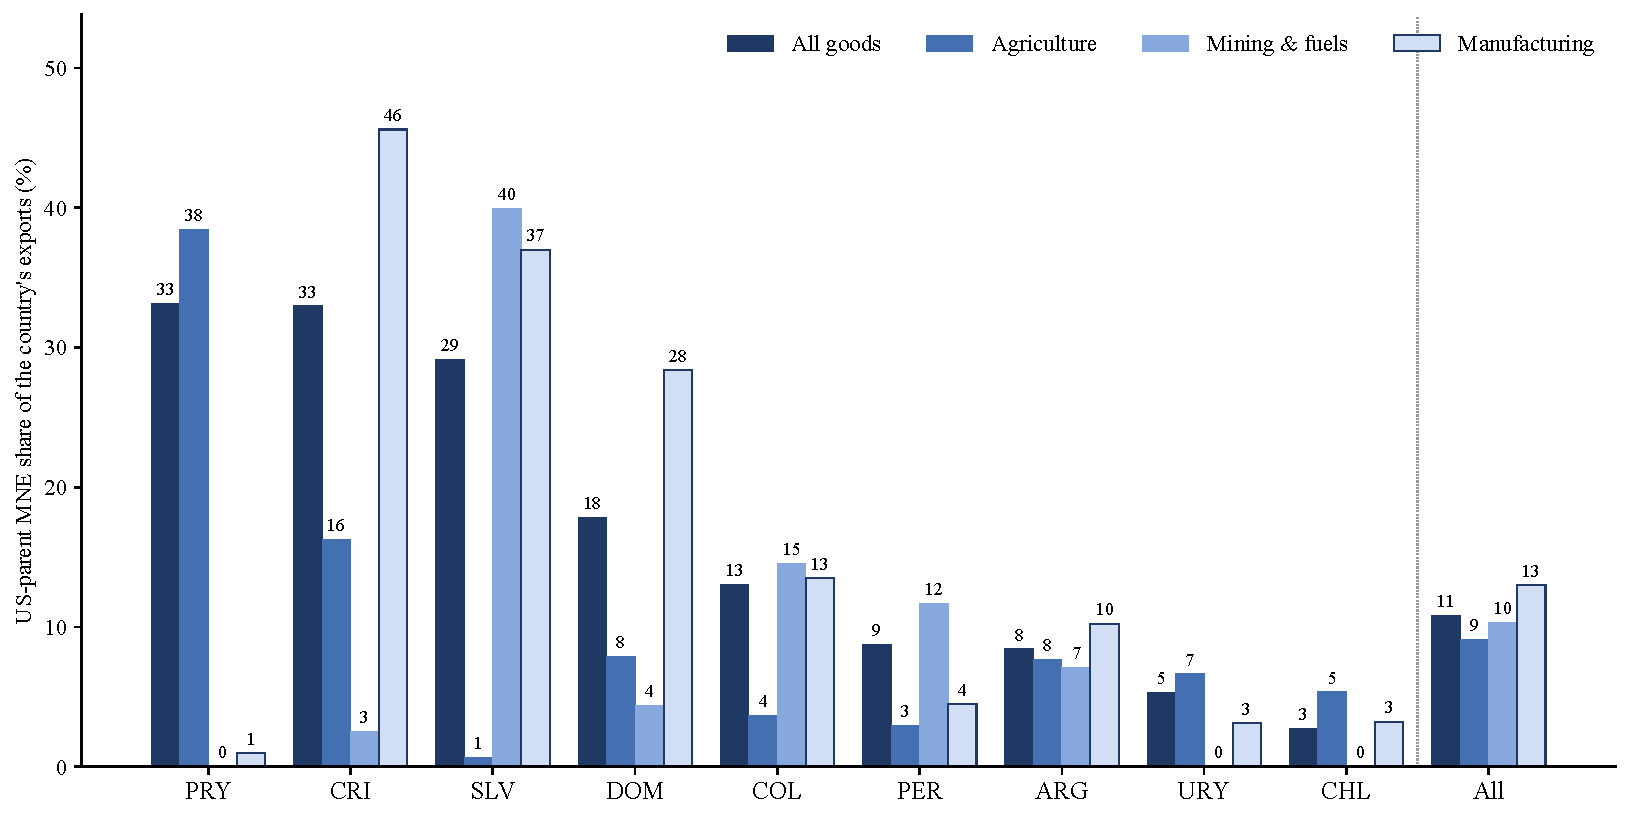
\includegraphics[width=1.0\textwidth,height=0.8\textheight,keepaspectratio]{figures/sectors/fig_wp3_us_share_origin_sector.pdf}%
  \caption{Exports by US-Parent Multinationals, by Exporting Country and Sector}%
  \label{fig:us_ox_sector}%
  \par\vspace{2pt}%
  \parbox{0.92\textwidth}{\footnotesize %
  \textit{Notes:} Percent of each country's exports in each sector shipped by US-parent MNEs, to all destinations.\\[3pt]%
  \textit{Source:} Authors' calculations based on customs data matched to Orbis and Dun \& Bradstreet.}%
  \end{figure}
% ---- Table: Exports by US-Parent Multinationals, by Exporting Country and Sector
\begin{table}[H]\centering\small%
  \caption{Exports by US-Parent Multinationals, by Exporting Country and Sector}%
  \label{tab:us_ox_sector_t}%
  \adjustbox{max width=\textwidth, max totalheight=0.8\textheight}{\begin{tabular}{lrrrrrrrr}
\toprule
 & \multicolumn{4}{c}{US-parent MNE share of the origin's exports in the sector (\%)} & \multicolumn{4}{c}{US-parent MNE exports (US\$bn/yr)} \\
Origin & All goods & Agriculture & Mining \& fuels & Manufacturing & All goods & Agriculture & Mining \& fuels & Manufacturing \\
\midrule
PRY & 33.1 & 38.5 & 0.0 & 1.0 & 2.2 & 2.2 & 0.0 & 0.0 \\
CRI & 33.0 & 16.2 & 2.6 & 45.6 & 3.2 & 0.6 & 0.0 & 2.5 \\
SLV & 29.1 & 0.6 & 39.9 & 37.0 & 1.4 & 0.0 & 0.1 & 1.3 \\
DOM & 17.8 & 7.9 & 4.4 & 28.4 & 1.5 & 0.2 & 0.1 & 1.2 \\
COL & 13.1 & 3.7 & 14.6 & 13.5 & 5.1 & 0.2 & 3.9 & 1.0 \\
PER & 8.8 & 2.9 & 11.7 & 4.5 & 3.2 & 0.2 & 2.8 & 0.3 \\
ARG & 8.4 & 7.7 & 7.1 & 10.2 & 5.4 & 2.7 & 0.5 & 2.2 \\
URY & 5.3 & 6.6 & 0.0 & 3.1 & 0.3 & 0.3 & 0.0 & 0.1 \\
CHL & 2.8 & 5.4 & 0.1 & 3.2 & 0.9 & 0.3 & 0.0 & 0.5 \\
\midrule
All & 10.8 & 9.1 & 10.3 & 13.0 & 23.1 & 6.7 & 7.3 & 9.1 \\
\bottomrule
\end{tabular}
}%
  \par\vspace{3pt}%
  \begin{minipage}{0.95\textwidth}\footnotesize %
  \textit{Notes:} Left panel: percent of each country's exports in the sector shipped by US-parent MNEs. Right panel: exports by US-parent MNEs. Values are annual averages in US\$ billion.\\[3pt]%
  \textit{Source:} Authors' calculations based on customs data matched to Orbis and Dun \& Bradstreet.%
  \end{minipage}%
  \end{table}
% ---- Figure: Exports to the United States and Exports by US-Parent Multinationals
\begin{figure}[H]\centering%
  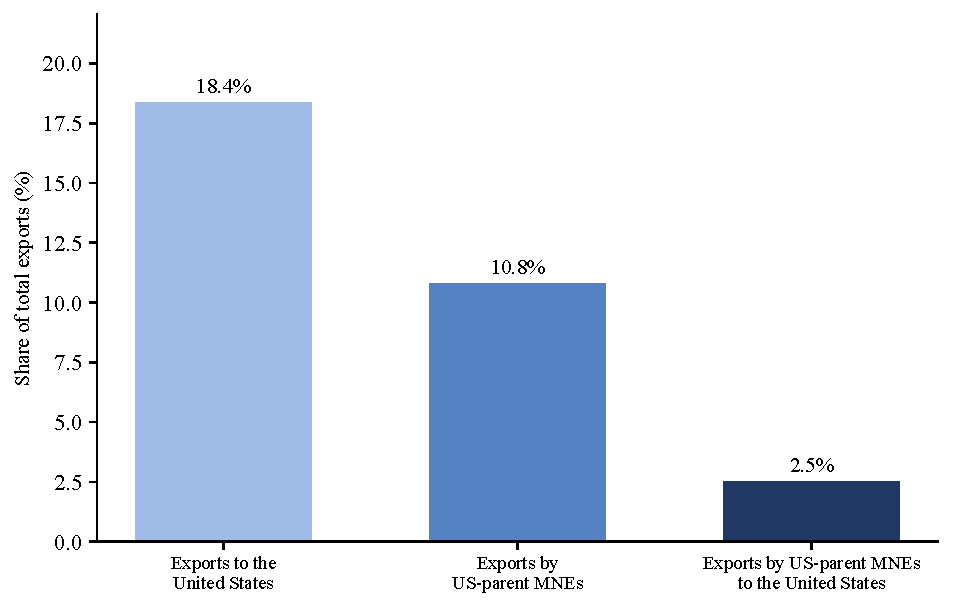
\includegraphics[width=0.6\textwidth,height=0.8\textheight,keepaspectratio]{figures/all/fig_wp3_us_three_shares_total.pdf}%
  \caption{Exports to the United States and Exports by US-Parent Multinationals}%
  \label{fig:us3_total}%
  \par\vspace{2pt}%
  \parbox{0.92\textwidth}{\footnotesize %
  \textit{Notes:} Shares of the total exports of the nine countries. The third bar is exports by US-parent MNEs shipped to the United States.\\[3pt]%
  \textit{Source:} Authors' calculations based on customs data matched to Orbis and Dun \& Bradstreet.}%
  \end{figure}
% ---- Figure: Exports to the United States and Exports by US-Parent Multinationals, by Exporting Country
\begin{figure}[H]\centering%
  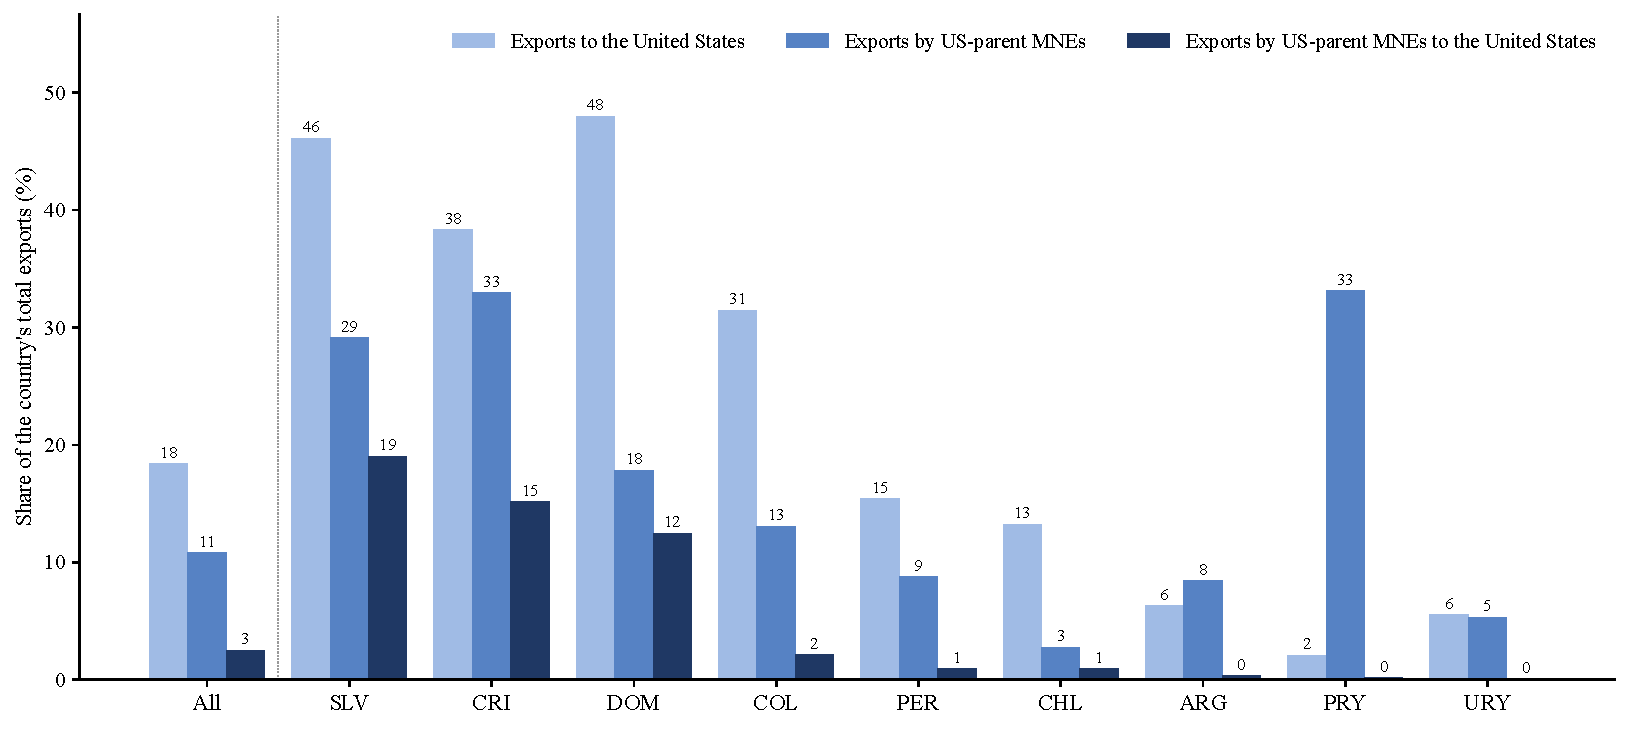
\includegraphics[width=1.0\textwidth,height=0.8\textheight,keepaspectratio]{figures/all/fig_wp3_us_three_shares_origin.pdf}%
  \caption{Exports to the United States and Exports by US-Parent Multinationals, by Exporting Country}%
  \label{fig:us3_origin}%
  \par\vspace{2pt}%
  \parbox{0.92\textwidth}{\footnotesize %
  \textit{Notes:} Shares of each country's total exports.\\[3pt]%
  \textit{Source:} Authors' calculations based on customs data matched to Orbis and Dun \& Bradstreet.}%
  \end{figure}
% ---- Table: Exports to the United States and Exports by US-Parent Multinationals, by Exporting Country
\begin{table}[H]\centering\small%
  \caption{Exports to the United States and Exports by US-Parent Multinationals, by Exporting Country}%
  \label{tab:us3_tab}%
  \adjustbox{max width=\textwidth, max totalheight=0.8\textheight}{\begin{tabular}{lrrrrr}
\toprule
Origin & \multicolumn{1}{p{2.3cm}}{\raggedright (1) \% of exports going to the USA} & \multicolumn{1}{p{2.3cm}}{\raggedright (2) \% of exports carried by US-parent MNEs} & \multicolumn{1}{p{2.6cm}}{\raggedright (3) \% of exports carried by US-parent MNEs and going to the USA} & \multicolumn{1}{p{2.6cm}}{\raggedright (4) = (3)/(1): US-parent share of the exports going to the USA (\%)} & \multicolumn{1}{p{1.8cm}}{\raggedright Total exports (US\$bn/yr)} \\
\midrule
All & 18.4 & 10.8 & 2.5 & 13.6 & 224.5 \\
\midrule
SLV & 46.1 & 29.1 & 19.0 & 41.3 & 5.0 \\
CRI & 38.3 & 33.0 & 15.1 & 39.5 & 10.5 \\
DOM & 48.0 & 17.8 & 12.5 & 26.0 & 8.6 \\
COL & 31.5 & 13.1 & 2.1 & 6.8 & 44.0 \\
PER & 15.4 & 8.8 & 0.9 & 6.0 & 41.4 \\
CHL & 13.3 & 2.8 & 0.9 & 6.9 & 34.2 \\
ARG & 6.3 & 8.4 & 0.3 & 5.5 & 66.4 \\
PRY & 2.1 & 33.1 & 0.2 & 8.1 & 7.3 \\
URY & 5.5 & 5.3 & 0.0 & 0.4 & 7.0 \\
\bottomrule
\end{tabular}
}%
  \par\vspace{3pt}%
  \begin{minipage}{0.95\textwidth}\footnotesize %
  \textit{Notes:} Columns (1)--(3): percent of each country's total exports. Column (4): percent of exports to the United States shipped by US-parent MNEs. Countries sorted by column (3). Values are annual averages in US\$ billion.\\[3pt]%
  \textit{Source:} Authors' calculations based on customs data matched to Orbis and Dun \& Bradstreet.%
  \end{minipage}%
  \end{table}

\section{Fact 2: Foreign Multinationals Specialize in Complex Products, Domestic Multinationals in Primary Goods}\label{sec:f2_all}

\subsection{Product Complexity and Technology}
% ---- Figure: Multinational Share of Export Value, by Product Complexity Quintile
\begin{figure}[H]\centering%
  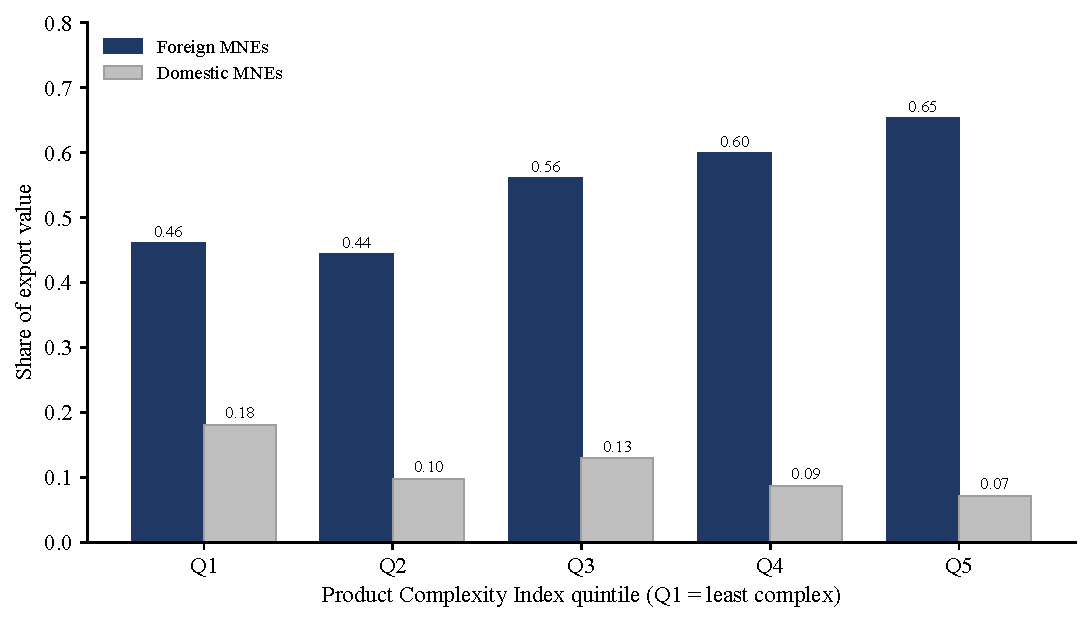
\includegraphics[width=0.78\textwidth,height=0.8\textheight,keepaspectratio]{figures/all/fig_wp0_fig2_pci.pdf}%
  \caption{Multinational Share of Export Value, by Product Complexity Quintile}%
  \label{fig:pci_all}%
  \par\vspace{2pt}%
  \parbox{0.92\textwidth}{\footnotesize %
  \textit{Notes:} Shares of export value, all available years pooled. Quintiles of the Hausmann--Hidalgo Product Complexity Index across HS6 products (Q1 = least complex).\\[3pt]%
  \textit{Source:} Authors' calculations based on customs data matched to Orbis and Dun \& Bradstreet.}%
  \end{figure}
% ---- Figure: Multinational Share of Export Value, by Technology Class
\begin{figure}[H]\centering%
  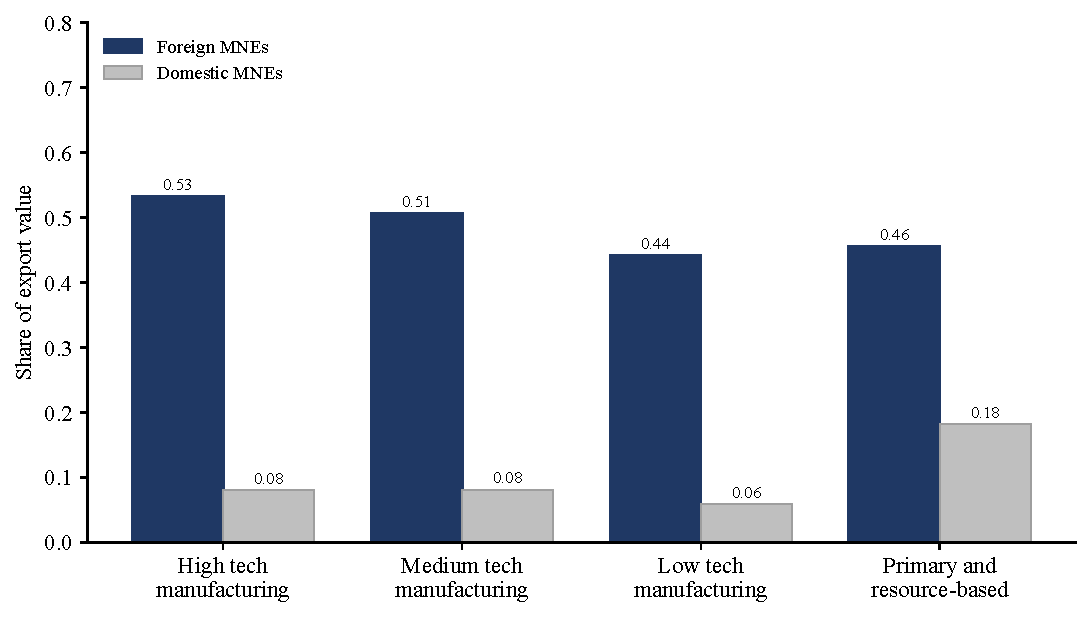
\includegraphics[width=0.78\textwidth,height=0.8\textheight,keepaspectratio]{figures/all/fig_wp0_fig3_lall.pdf}%
  \caption{Multinational Share of Export Value, by Technology Class}%
  \label{fig:lall_all}%
  \par\vspace{2pt}%
  \parbox{0.92\textwidth}{\footnotesize %
  \textit{Notes:} Shares of export value, all available years pooled. Lall (2000) technology classes: primary and resource-based products, and low-, medium- and high-technology manufactures.\\[3pt]%
  \textit{Source:} Authors' calculations based on customs data matched to Orbis and Dun \& Bradstreet.}%
  \end{figure}

\subsection{By Parent Country}
% ---- Figure: Multinational Share of Export Value, by Product Complexity Quintile and Parent Country
\begin{figure}[H]\centering%
  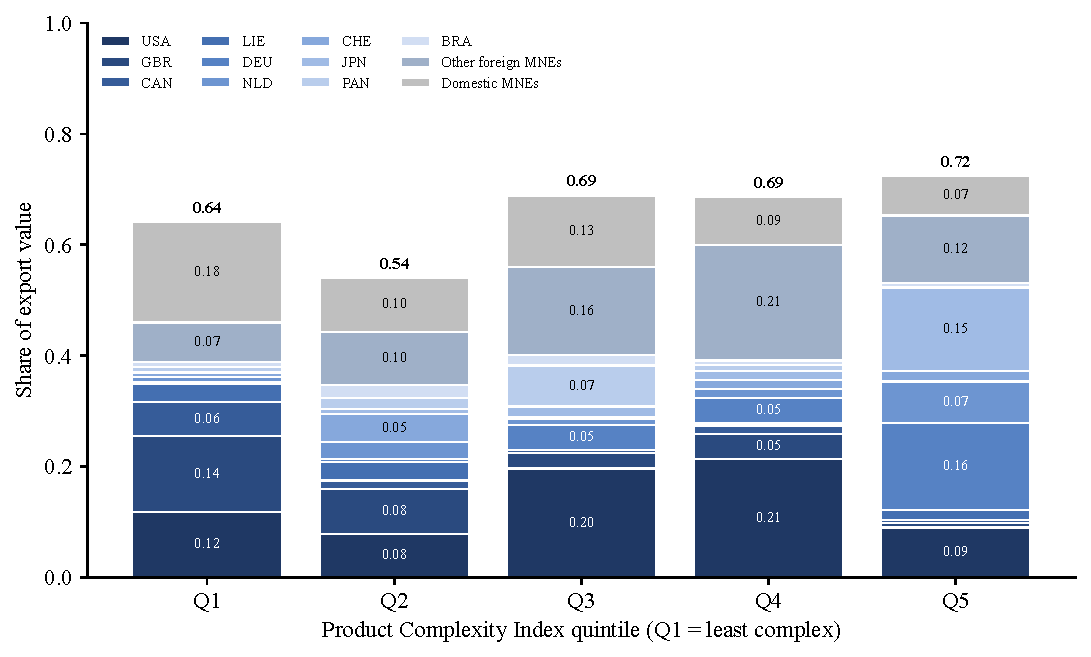
\includegraphics[width=0.92\textwidth,height=0.8\textheight,keepaspectratio]{figures/all/fig_wp1a_pci_by_parent.pdf}%
  \caption{Multinational Share of Export Value, by Product Complexity Quintile and Parent Country}%
  \label{fig:pci_p_all}%
  \par\vspace{2pt}%
  \parbox{0.92\textwidth}{\footnotesize %
  \textit{Notes:} Shares of export value, all available years pooled. Foreign MNEs split by country of the ultimate parent. Quintiles of the Hausmann--Hidalgo Product Complexity Index across HS6 products (Q1 = least complex).\\[3pt]%
  \textit{Source:} Authors' calculations based on customs data matched to Orbis and Dun \& Bradstreet.}%
  \end{figure}
% ---- Table: Multinational Share of Export Value, by Product Complexity Quintile and Parent Country
\begin{table}[H]\centering\small%
  \caption{Multinational Share of Export Value, by Product Complexity Quintile and Parent Country}%
  \label{tab:pci_pn_all}%
  \adjustbox{max width=\textwidth, max totalheight=0.8\textheight}{\begin{tabular}{lcccccccccccccc}
\toprule
PCI quintile & USA & GBR & CAN & LIE & DEU & NLD & CHE & JPN & PAN & BRA & Other & Domestic & All MNEs & Value (US\$bn/yr) \\
\midrule
Q1 & 0.118 & 0.137 & 0.061 & 0.034 & 0.002 & 0.010 & 0.008 & 0.001 & 0.009 & 0.008 & 0.072 & 0.181 & 0.641 & 106.7 \\
Q2 & 0.079 & 0.080 & 0.016 & 0.033 & 0.006 & 0.030 & 0.051 & 0.008 & 0.021 & 0.023 & 0.096 & 0.098 & 0.540 & 44.3 \\
Q3 & 0.196 & 0.028 & 0.005 & 0.000 & 0.045 & 0.010 & 0.005 & 0.018 & 0.074 & 0.019 & 0.159 & 0.129 & 0.689 & 13.4 \\
Q4 & 0.213 & 0.046 & 0.014 & 0.005 & 0.045 & 0.015 & 0.017 & 0.016 & 0.011 & 0.008 & 0.208 & 0.087 & 0.686 & 13.1 \\
Q5 & 0.090 & 0.008 & 0.005 & 0.018 & 0.157 & 0.074 & 0.019 & 0.150 & 0.002 & 0.007 & 0.122 & 0.071 & 0.724 & 14.4 \\
\bottomrule
\end{tabular}
}%
  \par\vspace{3pt}%
  \begin{minipage}{0.95\textwidth}\footnotesize %
  \textit{Notes:} Shares of export value, all available years pooled. Other: all remaining foreign parents. Values are annual averages in US\$ billion.\\[3pt]%
  \textit{Source:} Authors' calculations based on customs data matched to Orbis and Dun \& Bradstreet.%
  \end{minipage}%
  \end{table}
% ---- Figure: Multinational Share of Export Value, by Technology Class and Parent Country
\begin{figure}[H]\centering%
  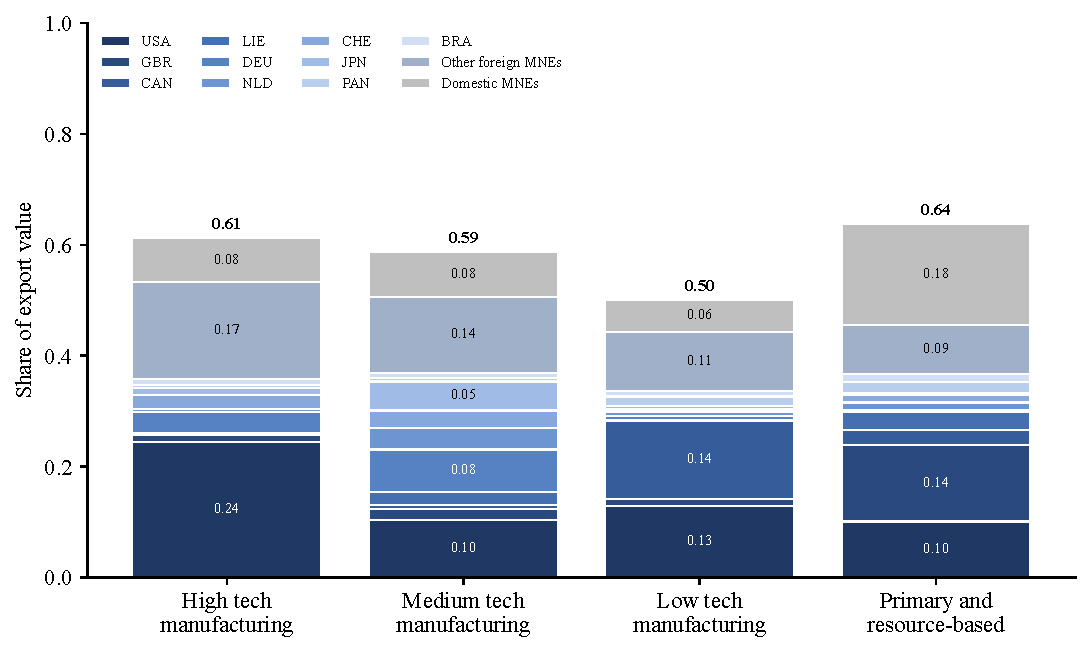
\includegraphics[width=0.92\textwidth,height=0.8\textheight,keepaspectratio]{figures/all/fig_wp1a_lall_by_parent.pdf}%
  \caption{Multinational Share of Export Value, by Technology Class and Parent Country}%
  \label{fig:lall_p_all}%
  \par\vspace{2pt}%
  \parbox{0.92\textwidth}{\footnotesize %
  \textit{Notes:} Shares of export value, all available years pooled. Foreign MNEs split by country of the ultimate parent. Lall (2000) technology classes: primary and resource-based products, and low-, medium- and high-technology manufactures.\\[3pt]%
  \textit{Source:} Authors' calculations based on customs data matched to Orbis and Dun \& Bradstreet.}%
  \end{figure}
% ---- Table: Multinational Share of Export Value, by Technology Class and Parent Country
\begin{table}[H]\centering\small%
  \caption{Multinational Share of Export Value, by Technology Class and Parent Country}%
  \label{tab:lall_pn_all}%
  \adjustbox{max width=\textwidth, max totalheight=0.8\textheight}{\begin{tabular}{lcccccccccccccc}
\toprule
Technology category & USA & GBR & CAN & LIE & DEU & NLD & CHE & JPN & PAN & BRA & Other & Domestic & All MNEs & Value (US\$bn/yr) \\
\midrule
High tech manufacturing & 0.244 & 0.014 & 0.003 & 0.000 & 0.037 & 0.005 & 0.025 & 0.012 & 0.006 & 0.010 & 0.175 & 0.080 & 0.613 & 6.0 \\
Medium tech manufacturing & 0.104 & 0.020 & 0.006 & 0.024 & 0.077 & 0.039 & 0.032 & 0.053 & 0.006 & 0.009 & 0.137 & 0.081 & 0.587 & 49.5 \\
Low tech manufacturing & 0.129 & 0.013 & 0.141 & 0.002 & 0.007 & 0.007 & 0.005 & 0.006 & 0.018 & 0.009 & 0.106 & 0.059 & 0.501 & 29.8 \\
Primary and resource-based & 0.101 & 0.138 & 0.027 & 0.032 & 0.003 & 0.014 & 0.014 & 0.004 & 0.019 & 0.015 & 0.089 & 0.182 & 0.638 & 130.9 \\
\bottomrule
\end{tabular}
}%
  \par\vspace{3pt}%
  \begin{minipage}{0.95\textwidth}\footnotesize %
  \textit{Notes:} Shares of export value, all available years pooled. Other: all remaining foreign parents. Values are annual averages in US\$ billion.\\[3pt]%
  \textit{Source:} Authors' calculations based on customs data matched to Orbis and Dun \& Bradstreet.%
  \end{minipage}%
  \end{table}
% ---- Figure: Multinational Share of Export Value, by Product Sophistication and Location of the Parent
\begin{figure}[H]\centering%
  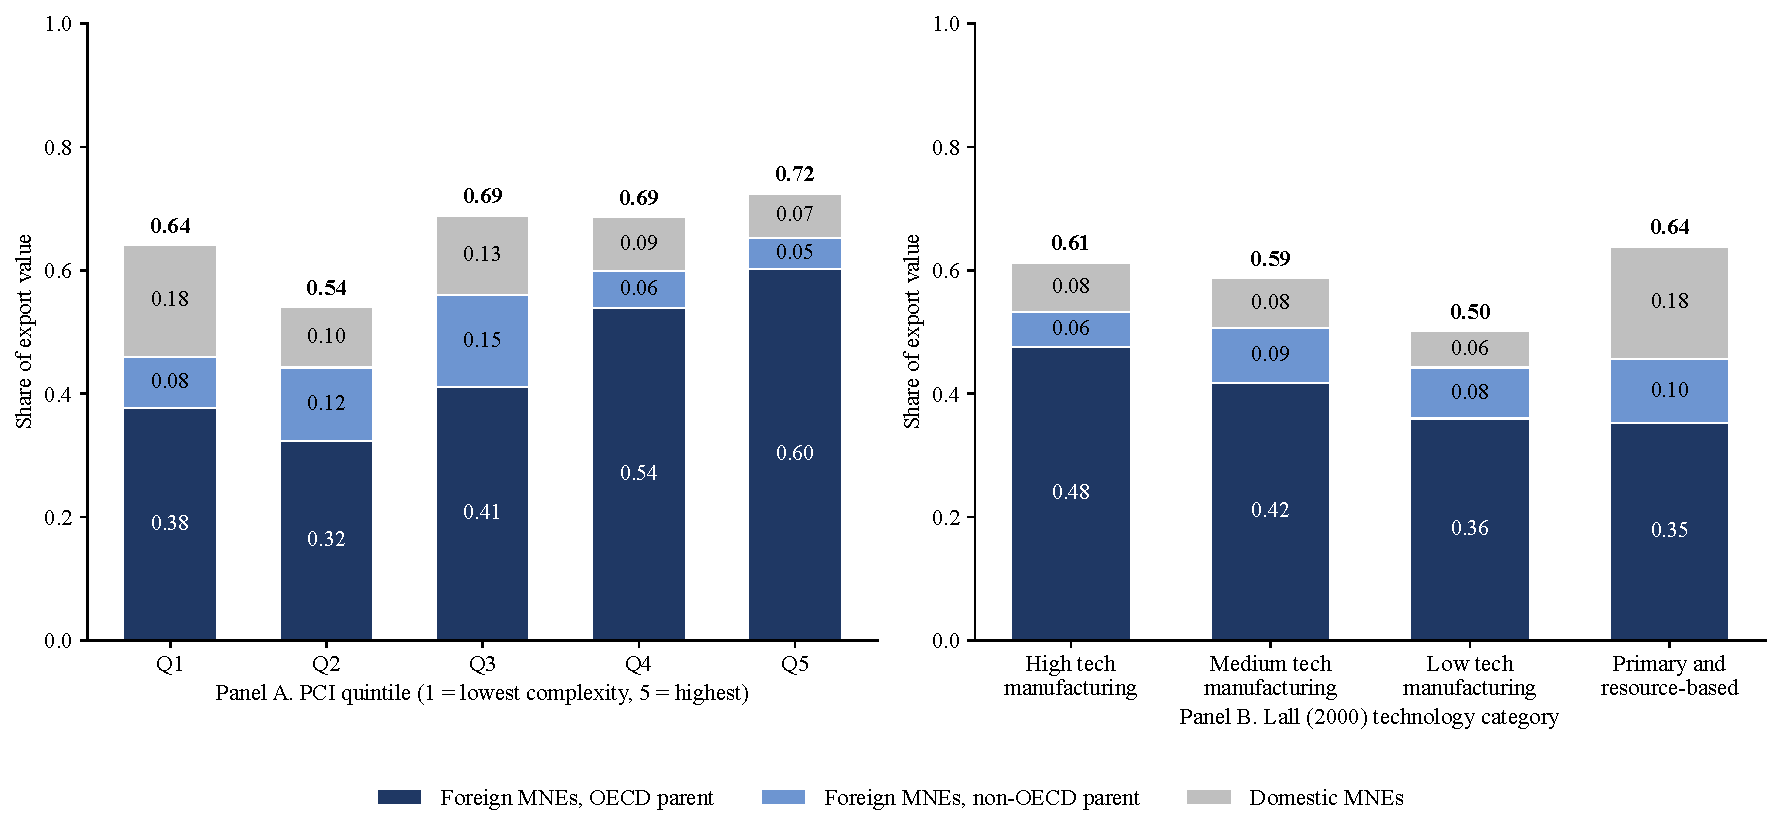
\includegraphics[width=1.0\textwidth,height=0.8\textheight,keepaspectratio]{figures/all/fig_wp1a_pci_lall_by_oecd.pdf}%
  \caption{Multinational Share of Export Value, by Product Sophistication and Location of the Parent}%
  \label{fig:oecd_all}%
  \par\vspace{2pt}%
  \parbox{0.92\textwidth}{\footnotesize %
  \textit{Notes:} Shares of export value, all available years pooled. Foreign MNEs are split by whether the ultimate parent is in an OECD member country. Panel A: Quintiles of the Hausmann--Hidalgo Product Complexity Index across HS6 products (Q1 = least complex). Panel B: Lall (2000) technology classes: primary and resource-based products, and low-, medium- and high-technology manufactures.\\[3pt]%
  \textit{Source:} Authors' calculations based on customs data matched to Orbis and Dun \& Bradstreet.}%
  \end{figure}

\subsection{Other Measures of Product Sophistication}
% ---- Figure: Multinational Share of Export Value, by Quintile of Six Sophistication Measures
\begin{figure}[H]\centering%
  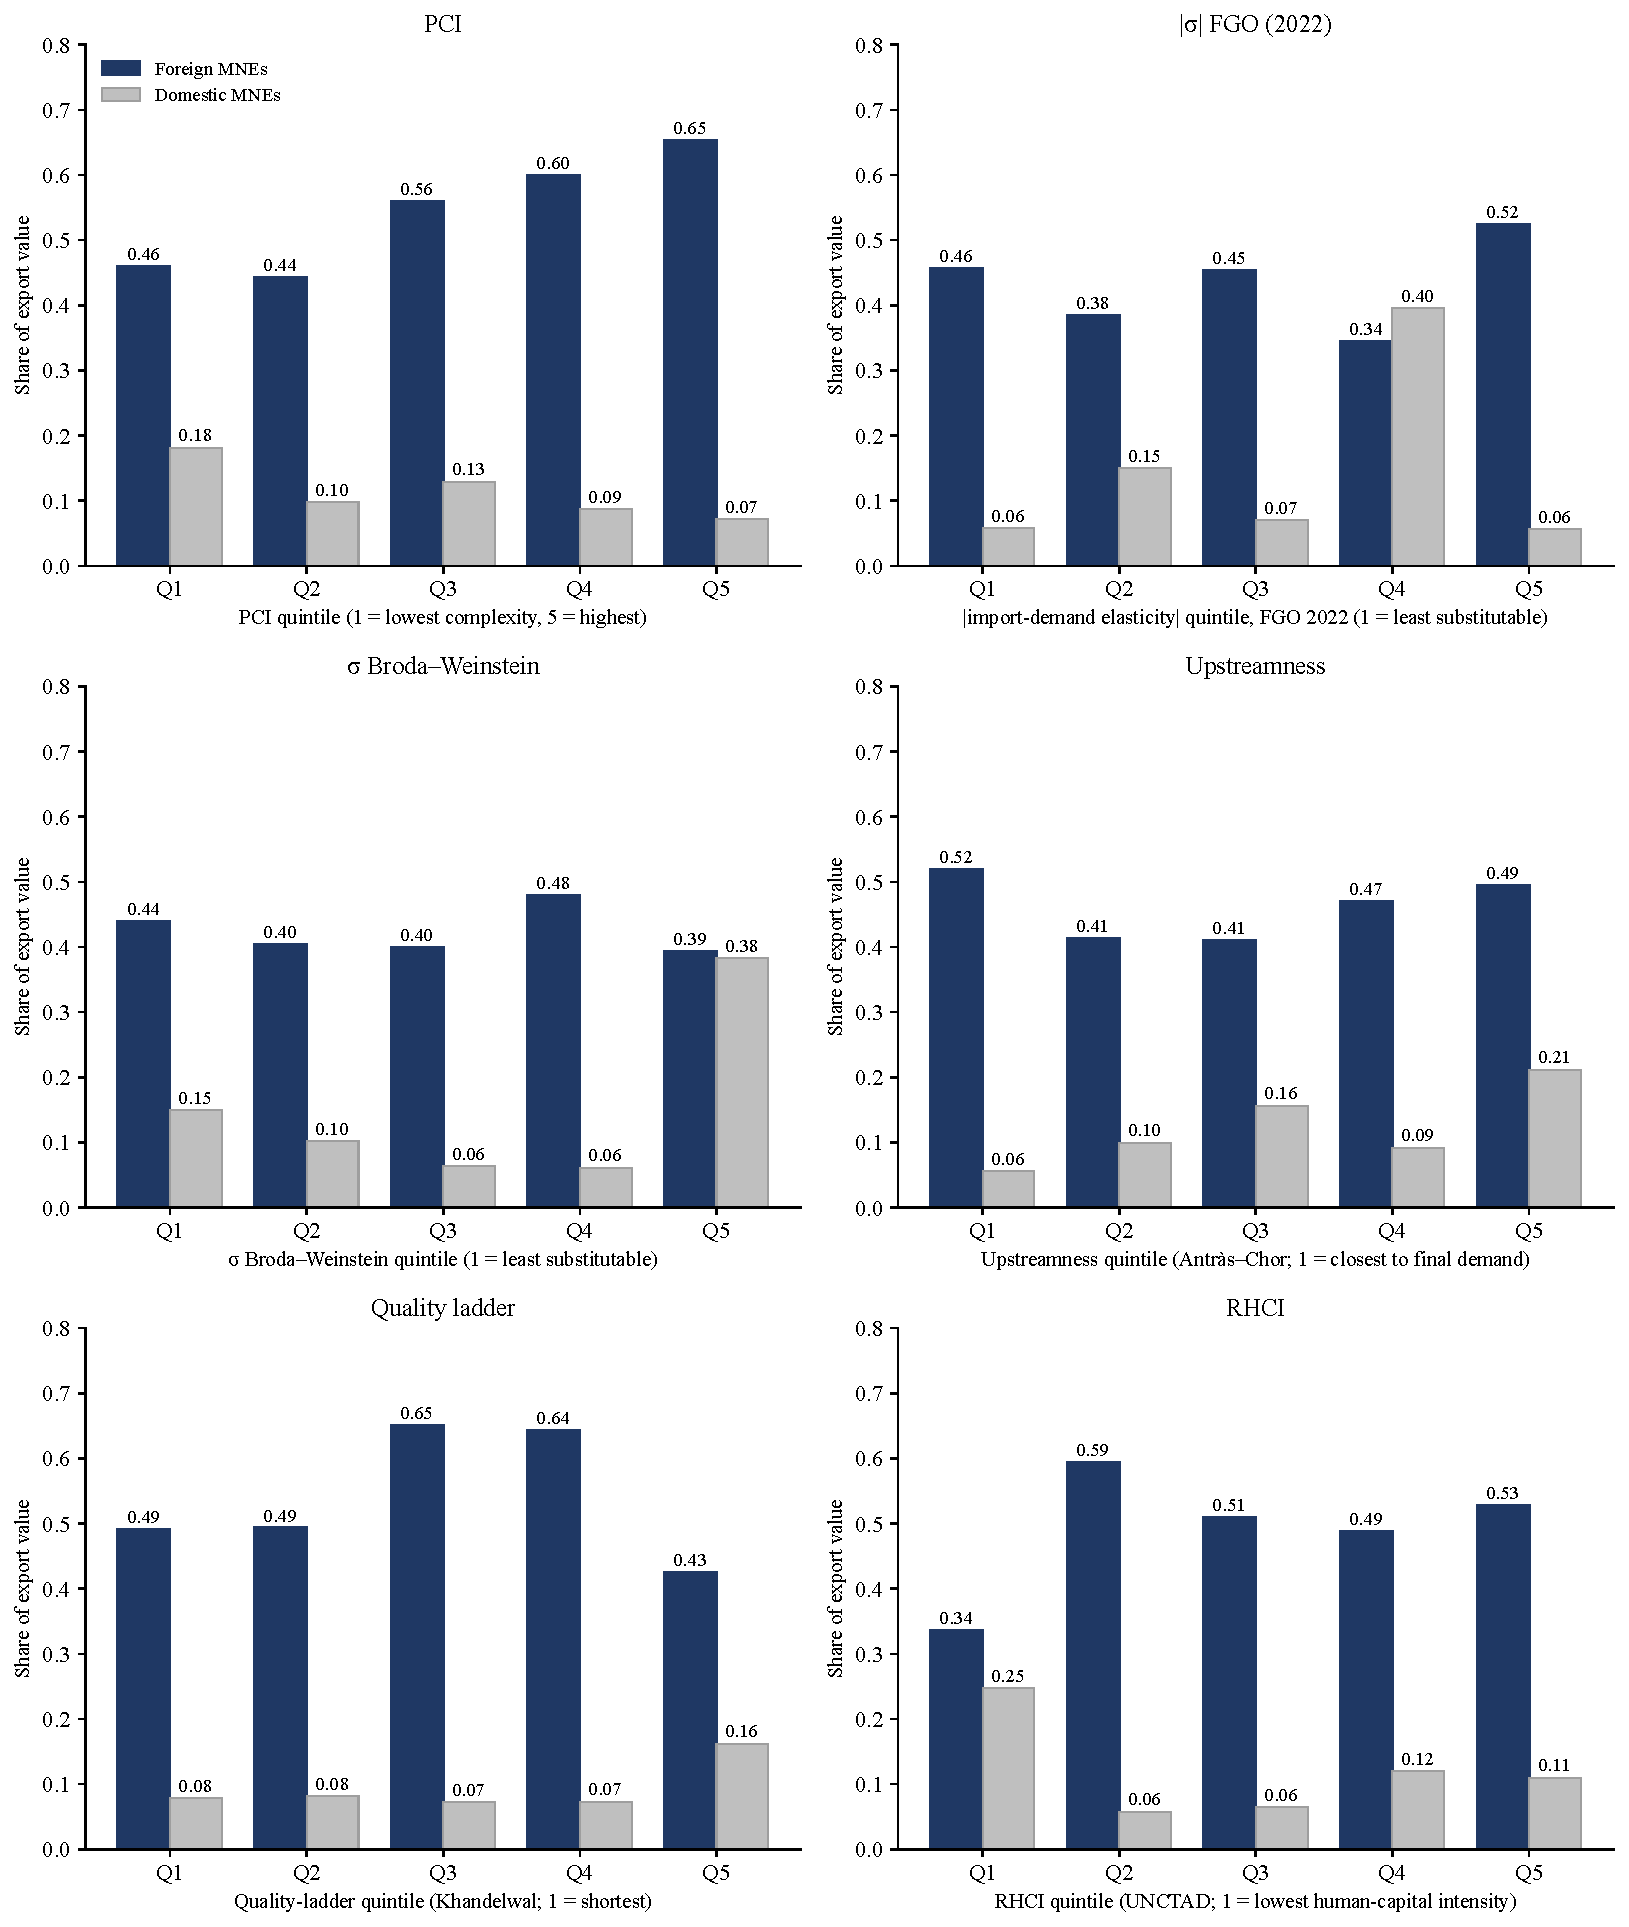
\includegraphics[width=1.0\textwidth,height=0.8\textheight,keepaspectratio]{figures/all/fig_wp1b_panel_quintiles.pdf}%
  \caption{Multinational Share of Export Value, by Quintile of Six Sophistication Measures}%
  \label{fig:six_q_all}%
  \par\vspace{2pt}%
  \parbox{0.92\textwidth}{\footnotesize %
  \textit{Notes:} Shares of export value, all available years pooled. Quintiles computed over HS6 products. The six measures are the Product Complexity Index, the absolute import-demand elasticity of Fontagn\'e, Guimbard and Orefice (2022), the elasticity of substitution of Broda and Weinstein, upstreamness, the quality ladder and the revealed human-capital intensity of UNCTAD.\\[3pt]%
  \textit{Source:} Authors' calculations based on customs data matched to Orbis and Dun \& Bradstreet.}%
  \end{figure}
% ---- Figure: Multinational Share of Export Value, by Quintile of the Import-Demand Elasticity
\begin{figure}[H]\centering%
  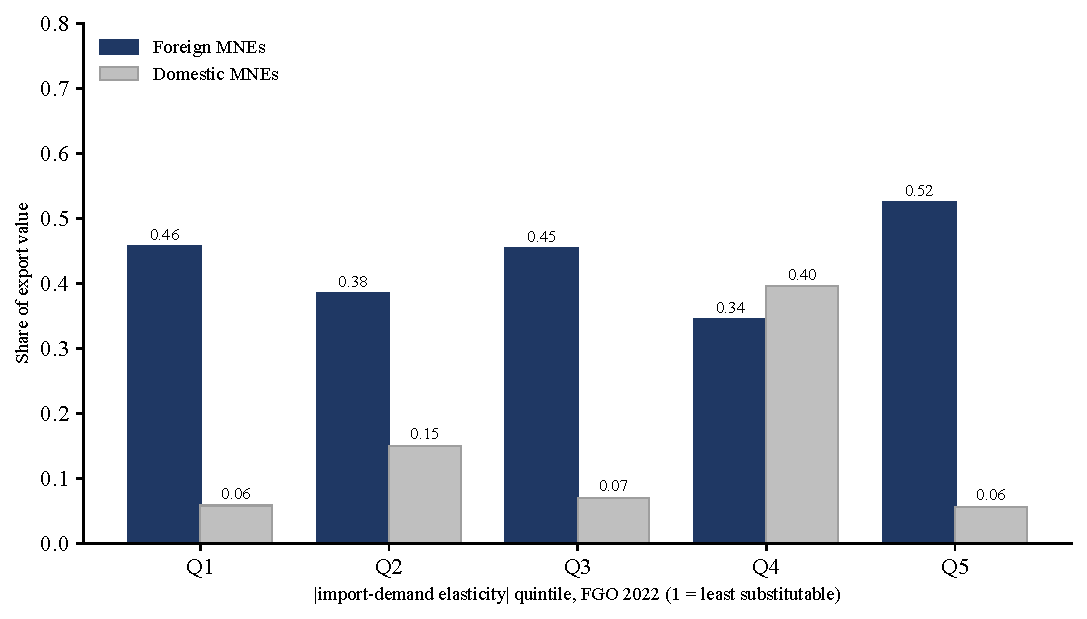
\includegraphics[width=0.78\textwidth,height=0.8\textheight,keepaspectratio]{figures/all/fig_wp1b_sigma_fgo_abs_quintile.pdf}%
  \caption{Multinational Share of Export Value, by Quintile of the Import-Demand Elasticity}%
  \label{fig:fgo_q_all}%
  \par\vspace{2pt}%
  \parbox{0.92\textwidth}{\footnotesize %
  \textit{Notes:} Shares of export value, all available years pooled. Quintiles of the absolute import-demand elasticity of Fontagn\'e, Guimbard and Orefice (2022) across HS6 products; higher quintiles are more substitutable products.\\[3pt]%
  \textit{Source:} Authors' calculations based on customs data matched to Orbis and Dun \& Bradstreet.}%
  \end{figure}
% ---- Figure: Distribution of Export Value across Six Sophistication Measures
\begin{figure}[H]\centering%
  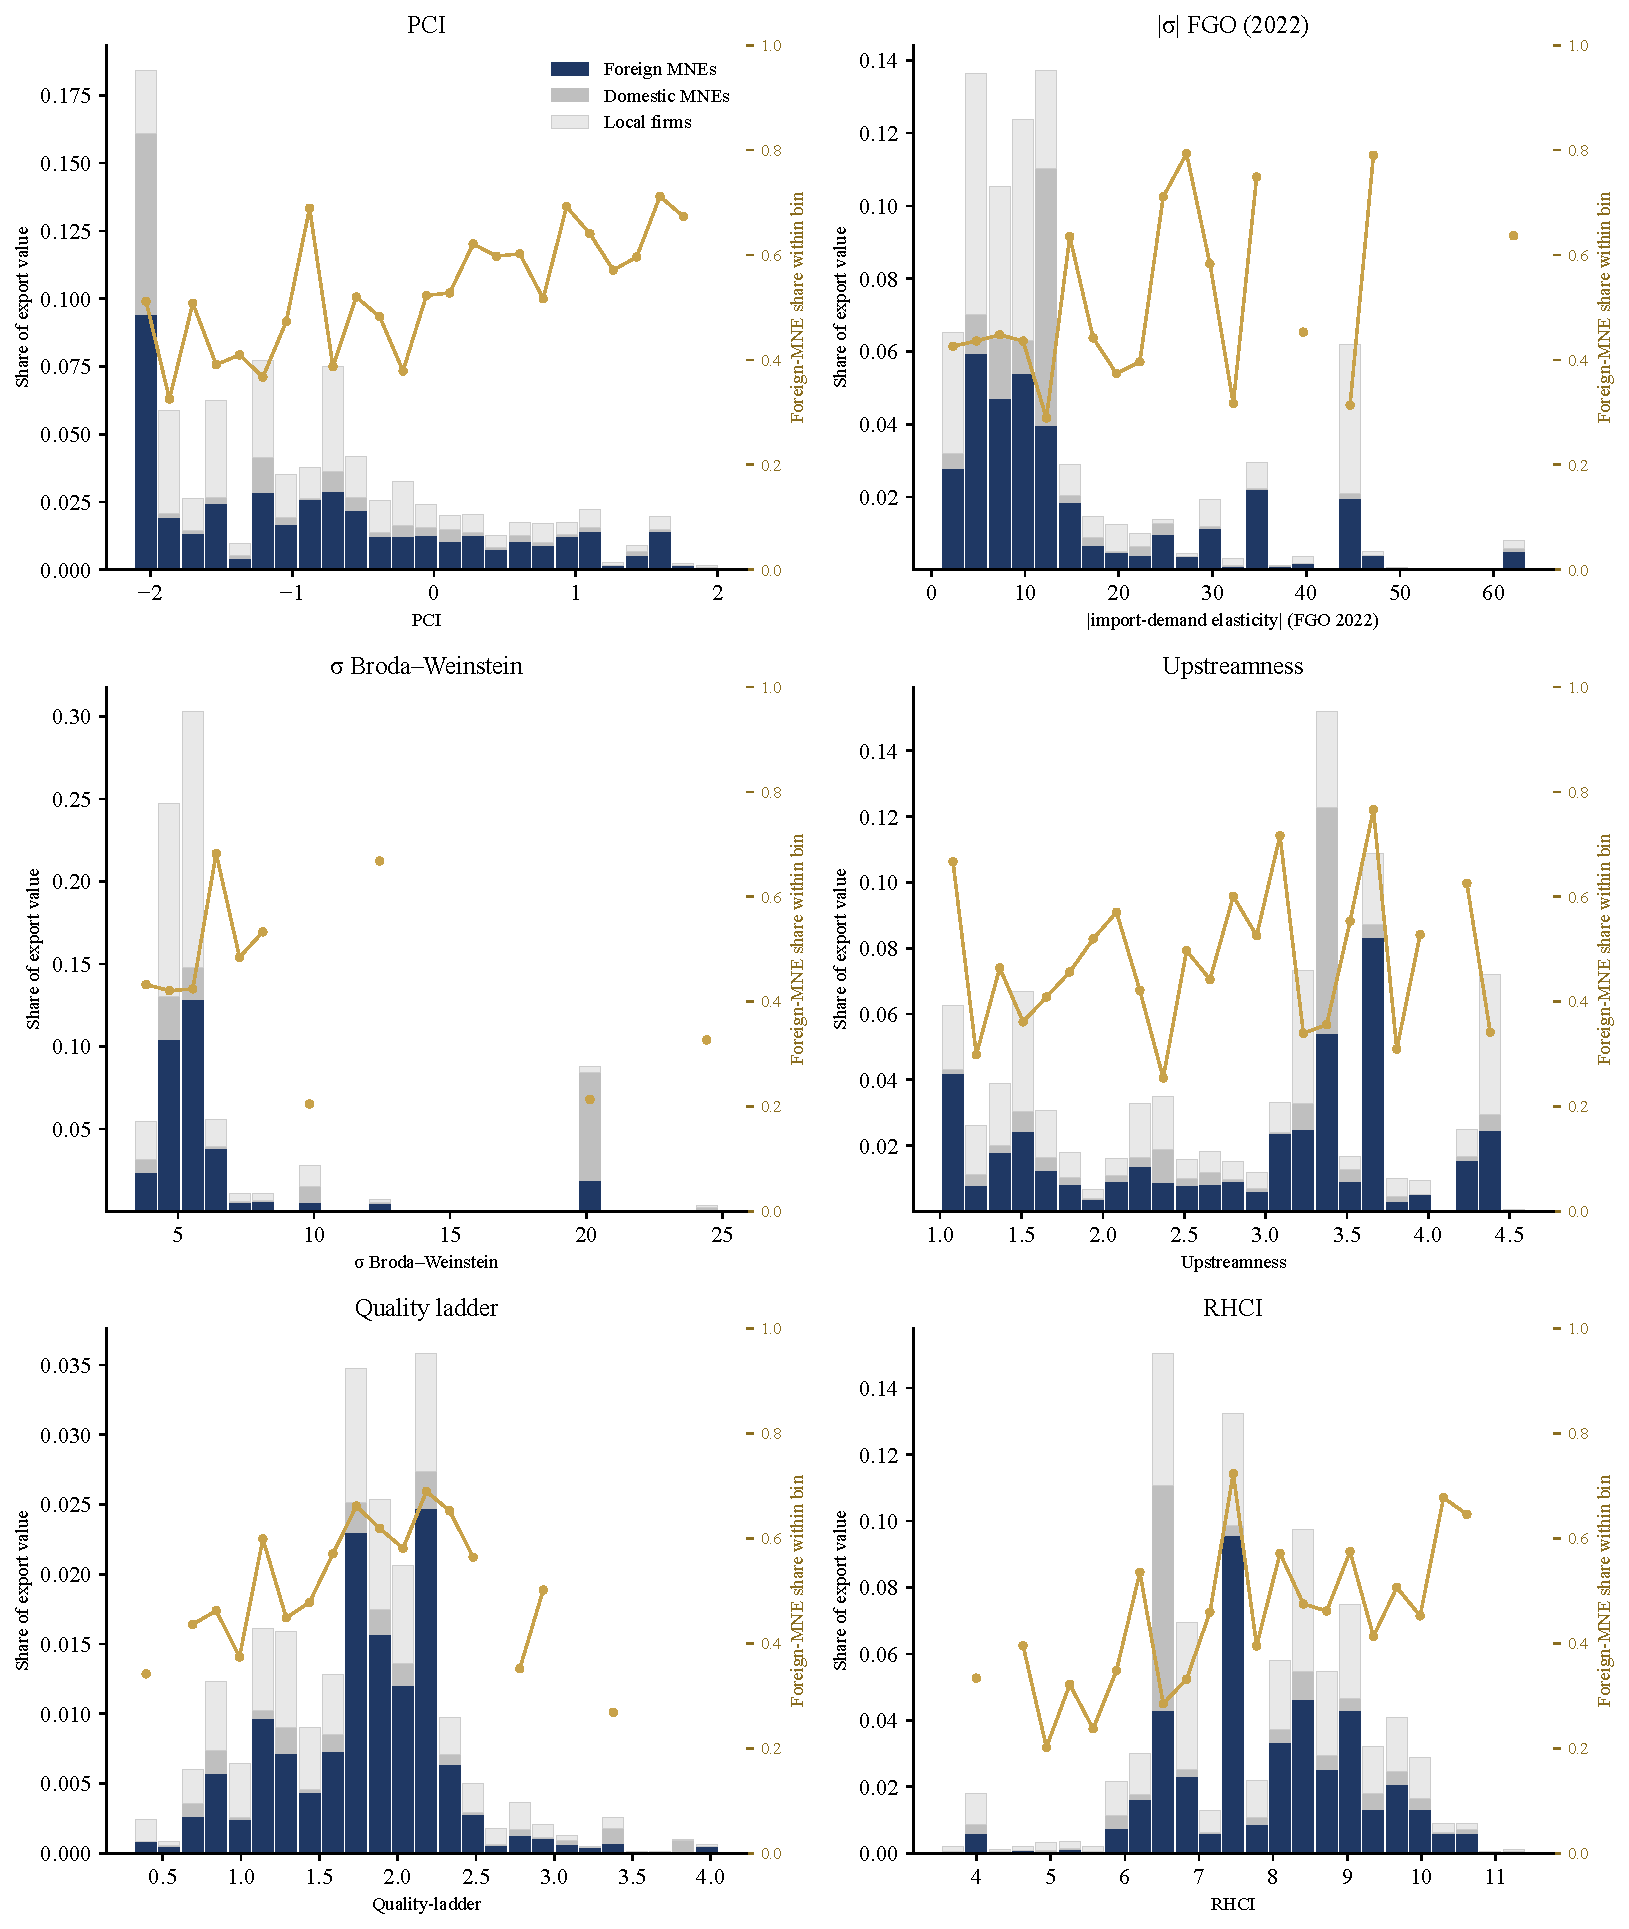
\includegraphics[width=1.0\textwidth,height=0.8\textheight,keepaspectratio]{figures/all/fig_wp1b_panel_hist.pdf}%
  \caption{Distribution of Export Value across Six Sophistication Measures}%
  \label{fig:six_h_all}%
  \par\vspace{2pt}%
  \parbox{0.92\textwidth}{\footnotesize %
  \textit{Notes:} Bars: export value in each bin, by type of exporter. Line (right axis): foreign-MNE share of each bin. The six measures are the Product Complexity Index, the absolute import-demand elasticity of Fontagn\'e, Guimbard and Orefice (2022), the elasticity of substitution of Broda and Weinstein, upstreamness, the quality ladder and the revealed human-capital intensity of UNCTAD.\\[3pt]%
  \textit{Source:} Authors' calculations based on customs data matched to Orbis and Dun \& Bradstreet.}%
  \end{figure}
% ---- Figure: Distribution of Export Value across the Import-Demand Elasticity
\begin{figure}[H]\centering%
  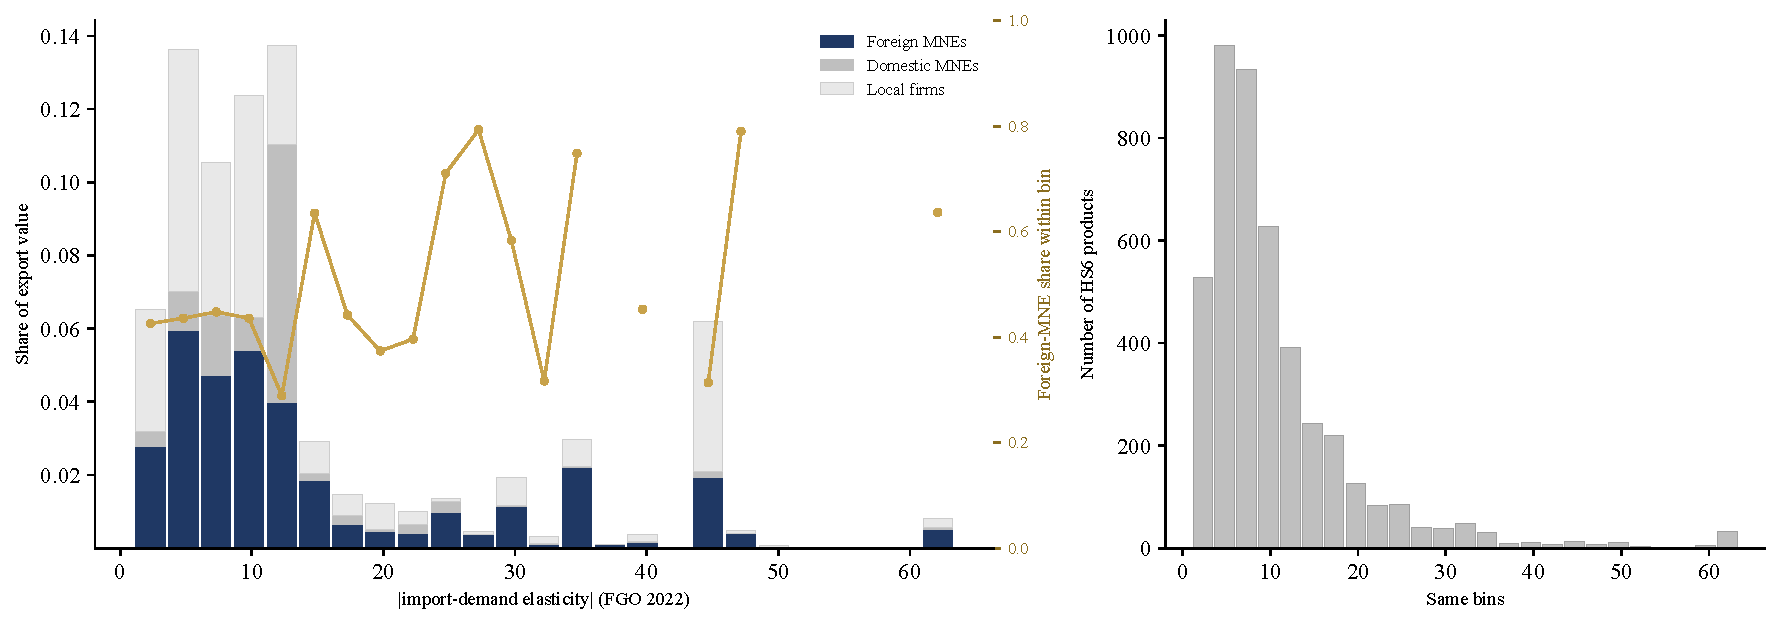
\includegraphics[width=1.0\textwidth,height=0.8\textheight,keepaspectratio]{figures/all/fig_wp1b_hist_sigma_fgo_abs.pdf}%
  \caption{Distribution of Export Value across the Import-Demand Elasticity}%
  \label{fig:fgo_h_all}%
  \par\vspace{2pt}%
  \parbox{0.92\textwidth}{\footnotesize %
  \textit{Notes:} Left: export value in each bin, by type of exporter, and the foreign-MNE share of each bin. Right: number of HS6 products in each bin.\\[3pt]%
  \textit{Source:} Authors' calculations based on customs data matched to Orbis and Dun \& Bradstreet.}%
  \end{figure}
% ---- Figure: Distribution of Export Value across the Product Complexity Index
\begin{figure}[H]\centering%
  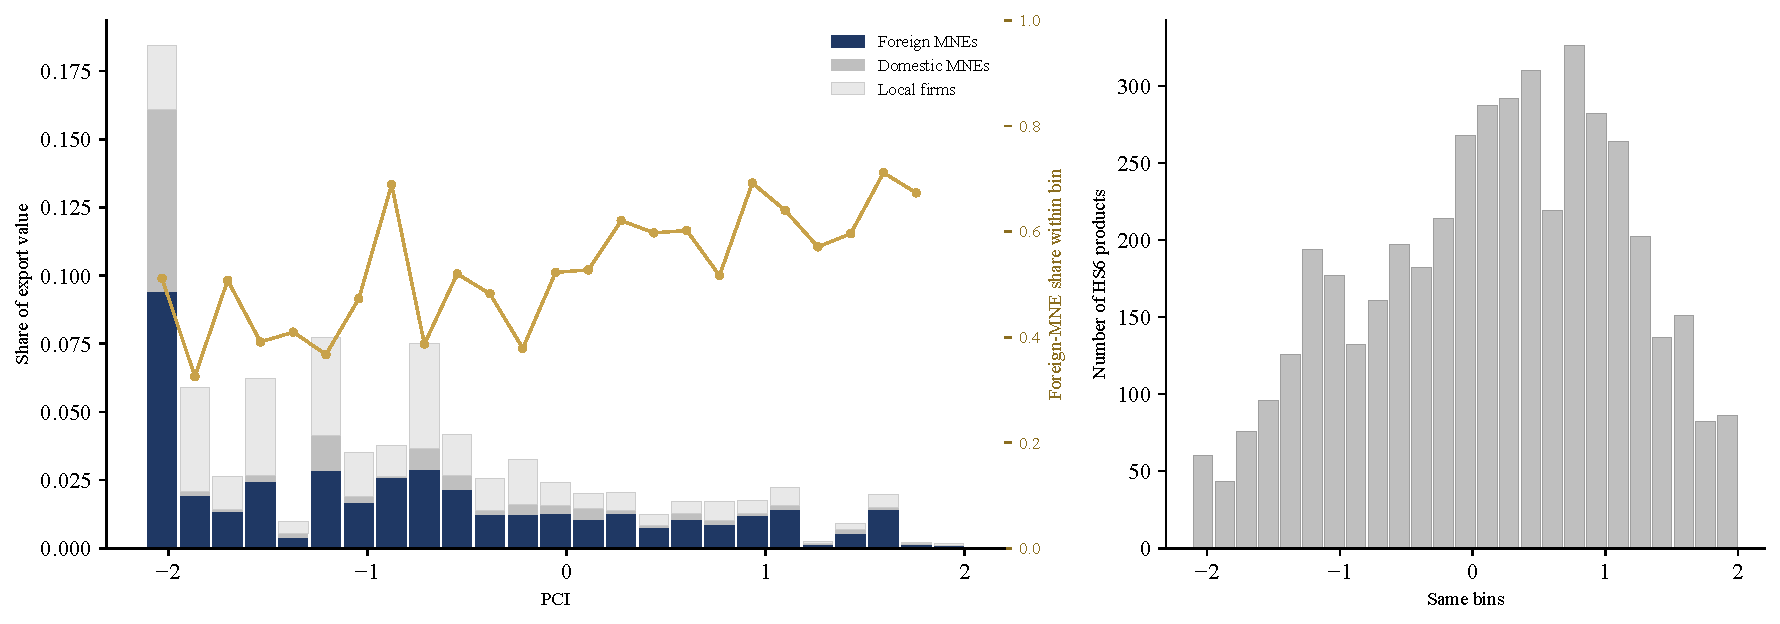
\includegraphics[width=1.0\textwidth,height=0.8\textheight,keepaspectratio]{figures/all/fig_wp1b_hist_complexity.pdf}%
  \caption{Distribution of Export Value across the Product Complexity Index}%
  \label{fig:pci_h_all}%
  \par\vspace{2pt}%
  \parbox{0.92\textwidth}{\footnotesize %
  \textit{Notes:} Left: export value in each bin, by type of exporter, and the foreign-MNE share of each bin. Right: number of HS6 products in each bin.\\[3pt]%
  \textit{Source:} Authors' calculations based on customs data matched to Orbis and Dun \& Bradstreet.}%
  \end{figure}
% ---- Table: Multinational Share of Export Value, by Quintile of Six Sophistication Measures
\begin{table}[H]\centering\small%
  \caption{Multinational Share of Export Value, by Quintile of Six Sophistication Measures}%
  \label{tab:six_t_all}%
  \adjustbox{max width=\textwidth, max totalheight=0.8\textheight}{\begin{tabular}{lccccc|ccccc}
\toprule
 & \multicolumn{5}{c}{Foreign MNE share} & \multicolumn{5}{c}{Domestic MNE share} \\
Measure & Q1 & Q2 & Q3 & Q4 & Q5 & Q1 & Q2 & Q3 & Q4 & Q5 \\
\midrule
PCI & 0.46 & 0.44 & 0.56 & 0.60 & 0.65 & 0.18 & 0.10 & 0.13 & 0.09 & 0.07 \\
$|\sigma|$ FGO (2022) & 0.46 & 0.38 & 0.45 & 0.34 & 0.52 & 0.06 & 0.15 & 0.07 & 0.40 & 0.06 \\
$\sigma$ Broda--Weinstein & 0.44 & 0.40 & 0.40 & 0.48 & 0.39 & 0.15 & 0.10 & 0.06 & 0.06 & 0.38 \\
Upstreamness & 0.52 & 0.41 & 0.41 & 0.47 & 0.49 & 0.06 & 0.10 & 0.16 & 0.09 & 0.21 \\
Quality ladder & 0.49 & 0.49 & 0.65 & 0.64 & 0.43 & 0.08 & 0.08 & 0.07 & 0.07 & 0.16 \\
RHCI & 0.34 & 0.59 & 0.51 & 0.49 & 0.53 & 0.25 & 0.06 & 0.06 & 0.12 & 0.11 \\
\bottomrule
\end{tabular}
}%
  \par\vspace{3pt}%
  \begin{minipage}{0.95\textwidth}\footnotesize %
  \textit{Notes:} Shares of export value, all available years pooled. Quintiles computed over HS6 products. --: fewer than 30 HS6 products carry the measure.\\[3pt]%
  \textit{Source:} Authors' calculations based on customs data matched to Orbis and Dun \& Bradstreet.%
  \end{minipage}%
  \end{table}
% ---- Table: Correlations between Sophistication Measures
\begin{table}[H]\centering\small%
  \caption{Correlations between Sophistication Measures}%
  \label{tab:corr_all}%
  \adjustbox{max width=\textwidth, max totalheight=0.8\textheight}{\begin{tabular}{lrrrrrr}
\toprule
 & PCI & $|\sigma|$ FGO (2022) & $\sigma$ Broda--Weinstein & Upstreamness & Quality ladder & RHCI \\
\midrule
PCI & 1.00 & -0.22 & -0.49 & -0.49 & 0.28 & 0.74 \\
$|\sigma|$ FGO (2022) & -0.22 & 1.00 & 0.03 & 0.62 & 0.12 & 0.02 \\
$\sigma$ Broda--Weinstein & -0.49 & 0.03 & 1.00 & 0.20 & -0.11 & -0.25 \\
Upstreamness & -0.49 & 0.62 & 0.20 & 1.00 & 0.12 & -0.19 \\
Quality ladder & 0.28 & 0.12 & -0.11 & 0.12 & 1.00 & 0.34 \\
RHCI & 0.74 & 0.02 & -0.25 & -0.19 & 0.34 & 1.00 \\
\bottomrule
\end{tabular}
}%
  \par\vspace{3pt}%
  \begin{minipage}{0.95\textwidth}\footnotesize %
  \textit{Notes:} Correlations across HS6 products, weighted by export value.\\[3pt]%
  \textit{Source:} Authors' calculations based on customs data matched to Orbis and Dun \& Bradstreet.%
  \end{minipage}%
  \end{table}

\subsection{Rauch Classes and End Use}
% ---- Table: Multinational Share of Export Value, by Rauch Product Class
\begin{table}[H]\centering\small%
  \caption{Multinational Share of Export Value, by Rauch Product Class}%
  \label{tab:rauch_all}%
  \adjustbox{max width=\textwidth, max totalheight=0.8\textheight}{\begin{tabular}{lcccrr}
\toprule
Rauch (1999) class & Foreign & Domestic & All MNEs & HS6 products & Value (US\$bn/yr) \\
\midrule
Differentiated & 0.563 & 0.058 & 0.621 & 2,712 & 44.3 \\
Reference-priced & 0.549 & 0.082 & 0.631 & 1,636 & 63.7 \\
Homogeneous (exchange) & 0.343 & 0.228 & 0.571 & 319 & 97.6 \\
\bottomrule
\end{tabular}
}%
  \par\vspace{3pt}%
  \begin{minipage}{0.95\textwidth}\footnotesize %
  \textit{Notes:} Shares of export value, all available years pooled. Rauch (1999) conservative classification: homogeneous goods are traded on organized exchanges, reference-priced goods have a price quoted in trade publications, and differentiated goods have neither. Values are annual averages in US\$ billion.\\[3pt]%
  \textit{Source:} Authors' calculations based on customs data matched to Orbis and Dun \& Bradstreet.%
  \end{minipage}%
  \end{table}
% ---- Figure: Multinational Share of Export Value, by Rauch Product Class
\begin{figure}[H]\centering%
  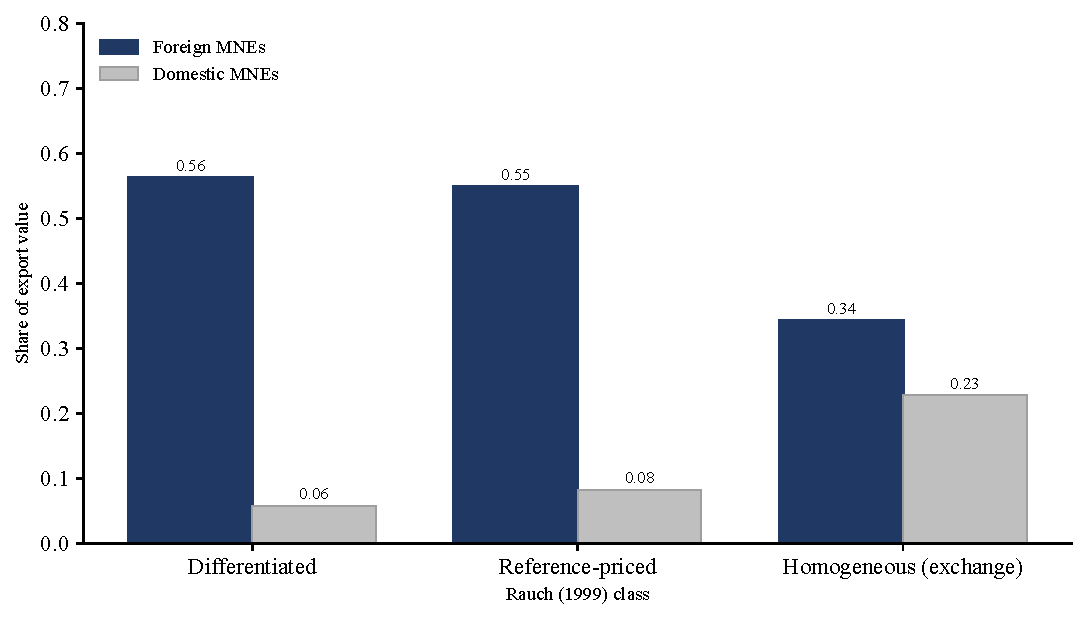
\includegraphics[width=0.7\textwidth,height=0.8\textheight,keepaspectratio]{figures/all/fig_wp1b_rauch.pdf}%
  \caption{Multinational Share of Export Value, by Rauch Product Class}%
  \label{fig:rauch_f_all}%
  \par\vspace{2pt}%
  \parbox{0.92\textwidth}{\footnotesize %
  \textit{Notes:} Shares of export value, all available years pooled. Rauch (1999) conservative classification: homogeneous goods are traded on organized exchanges, reference-priced goods have a price quoted in trade publications, and differentiated goods have neither.\\[3pt]%
  \textit{Source:} Authors' calculations based on customs data matched to Orbis and Dun \& Bradstreet.}%
  \end{figure}
% ---- Table: Multinational Share of Export Value: Differentiated and Other Products
\begin{table}[H]\centering\small%
  \caption{Multinational Share of Export Value: Differentiated and Other Products}%
  \label{tab:rauch2_all}%
  \adjustbox{max width=\textwidth, max totalheight=0.8\textheight}{\begin{tabular}{lcccrr}
\toprule
Rauch (1999): differentiated vs non-differentiated & Foreign & Domestic & All MNEs & HS6 products & Value (US\$bn/yr) \\
\midrule
Differentiated & 0.563 & 0.058 & 0.621 & 2,712 & 44.3 \\
Non-differentiated & 0.426 & 0.169 & 0.595 & 1,955 & 161.4 \\
\bottomrule
\end{tabular}
}%
  \par\vspace{3pt}%
  \begin{minipage}{0.95\textwidth}\footnotesize %
  \textit{Notes:} Shares of export value, all available years pooled. Rauch (1999) conservative classification; other products are reference-priced and homogeneous goods. Values are annual averages in US\$ billion.\\[3pt]%
  \textit{Source:} Authors' calculations based on customs data matched to Orbis and Dun \& Bradstreet.%
  \end{minipage}%
  \end{table}
% ---- Figure: Multinational Share of Export Value: Differentiated and Other Products
\begin{figure}[H]\centering%
  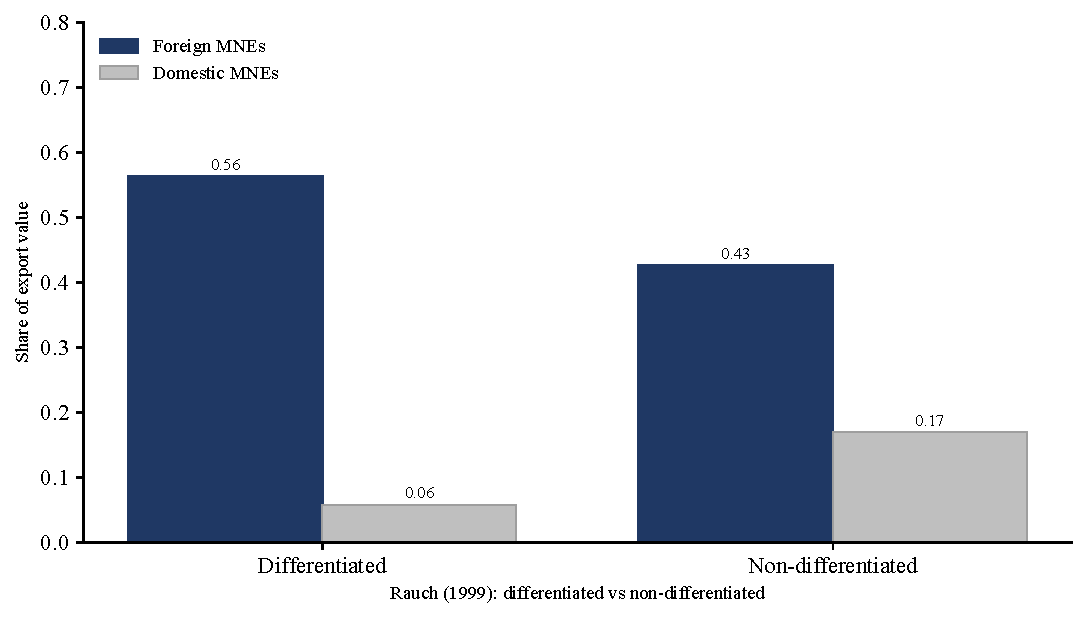
\includegraphics[width=0.7\textwidth,height=0.8\textheight,keepaspectratio]{figures/all/fig_wp1b_rauch2.pdf}%
  \caption{Multinational Share of Export Value: Differentiated and Other Products}%
  \label{fig:rauch2_f_all}%
  \par\vspace{2pt}%
  \parbox{0.92\textwidth}{\footnotesize %
  \textit{Notes:} Shares of export value, all available years pooled. Rauch (1999) conservative classification; other products are reference-priced and homogeneous goods.\\[3pt]%
  \textit{Source:} Authors' calculations based on customs data matched to Orbis and Dun \& Bradstreet.}%
  \end{figure}
% ---- Table: Multinational Share of Export Value, by End Use
\begin{table}[H]\centering\small%
  \caption{Multinational Share of Export Value, by End Use}%
  \label{tab:bec_all}%
  \adjustbox{max width=\textwidth, max totalheight=0.8\textheight}{\begin{tabular}{lcccrr}
\toprule
BEC end use & Foreign & Domestic & All MNEs & HS6 products & Value (US\$bn/yr) \\
\midrule
Intermediate & 0.476 & 0.155 & 0.631 & 3,090 & 155.0 \\
Consumption & 0.438 & 0.082 & 0.520 & 1,201 & 46.1 \\
Capital & 0.647 & 0.056 & 0.703 & 659 & 9.3 \\
\bottomrule
\end{tabular}
}%
  \par\vspace{3pt}%
  \begin{minipage}{0.95\textwidth}\footnotesize %
  \textit{Notes:} Shares of export value, all available years pooled. End use from BEC Rev.\,4; HS6 products without a BEC correspondence are excluded. Values are annual averages in US\$ billion.\\[3pt]%
  \textit{Source:} Authors' calculations based on customs data matched to Orbis and Dun \& Bradstreet.%
  \end{minipage}%
  \end{table}

\subsection{Regressions}
% ---- Table: Product Characteristics and Multinational Shares
\begin{table}[H]\centering\small%
  \caption{Product Characteristics and Multinational Shares}%
  \label{tab:fgo_r_all}%
  \adjustbox{max width=\textwidth, max totalheight=0.8\textheight}{\begin{tabular}{lccc} \hline
 & (1) & (2) & (3) \\ \hline
\multicolumn{4}{l}{\textit{Panel A. Dependent variable: share of all MNEs}} \\
Complexity (PCI) & 0.0281*** & 0.0307*** & 0.0409*** \\
 & (0.0047) & (0.0045) & (0.0040) \\
$|\sigma|$ FGO (per s.d.) & -0.0078*** & -0.0074*** & -0.0057*** \\
 & (0.0026) & (0.0025) & (0.0021) \\
Upstreamness & 0.0087* & 0.0079* & 0.0108*** \\
 & (0.0047) & (0.0044) & (0.0038) \\
\midrule
\multicolumn{4}{l}{\textit{Panel B. Dependent variable: share of foreign MNEs}} \\
Complexity (PCI) & 0.0926*** & 0.0925*** & 0.0855*** \\
 & (0.0049) & (0.0047) & (0.0043) \\
$|\sigma|$ FGO (per s.d.) & 0.0339*** & 0.0331*** & 0.0241*** \\
 & (0.0023) & (0.0022) & (0.0020) \\
Upstreamness & -0.0239*** & -0.0253*** & -0.0148*** \\
 & (0.0043) & (0.0041) & (0.0034) \\
\midrule
\multicolumn{4}{l}{\textit{Panel C. Dependent variable: share of domestic MNEs}} \\
Complexity (PCI) & -0.0645*** & -0.0618*** & -0.0446*** \\
 & (0.0053) & (0.0048) & (0.0038) \\
$|\sigma|$ FGO (per s.d.) & -0.0417*** & -0.0405*** & -0.0298*** \\
 & (0.0027) & (0.0025) & (0.0022) \\
Upstreamness & 0.0326*** & 0.0332*** & 0.0256*** \\
 & (0.0041) & (0.0037) & (0.0028) \\
\hline
Origin FE & $\checkmark$ &  &  \\
Destination FE & $\checkmark$ &  &  \\
Year FE & $\checkmark$ &  &  \\
Origin $\times$ year FE &  & $\checkmark$ &  \\
Destination $\times$ year FE &  & $\checkmark$ &  \\
Origin $\times$ dest.\ $\times$ year FE &  &  & $\checkmark$ \\
Observations & 1,563,005 & 1,562,745 & 1,561,136 \\
\hline
\end{tabular}
}%
  \par\vspace{3pt}%
  \begin{minipage}{0.95\textwidth}\footnotesize %
  \textit{Notes:} Observations are origin--destination--HS6--year cells. Dependent variable: share of the cell's export value shipped by each type of MNE. The import-demand elasticity is standardized (mean 0, standard deviation 1). Regressions weighted by the cell's export value. Robust standard errors in parentheses. *** $p<0.01$, ** $p<0.05$, * $p<0.1$.\\[3pt]%
  \textit{Source:} Authors' calculations based on customs data matched to Orbis and Dun \& Bradstreet.%
  \end{minipage}%
  \end{table}
% ---- Table: Product Sophistication and Multinational Shares
\begin{table}[H]\centering\footnotesize%
  \caption{Product Sophistication and Multinational Shares}%
  \label{tab:meas_r_all}%
  \adjustbox{max width=\textwidth, max totalheight=0.8\textheight}{\begin{tabular}{lcccccc} \hline
 & \multicolumn{2}{c}{PCI} & \multicolumn{2}{c}{Lall} & \multicolumn{2}{c}{Rauch} \\
 & (1) & (2) & (3) & (4) & (5) & (6) \\ \hline
\multicolumn{7}{l}{\textit{Panel A. Dependent variable: share of all MNEs}} \\
Complexity (PCI) & -0.0004 & 0.0052 &  &  &  &  \\
 & (0.0050) & (0.0045) &  &  &  &  \\
Lall: high tech (vs primary and resource-based) &  &  & -0.0288** & -0.0347** &  &  \\
 &  &  & (0.0142) & (0.0142) &  &  \\
Lall: medium tech &  &  & -0.0256*** & -0.0111 &  &  \\
 &  &  & (0.0081) & (0.0074) &  &  \\
Lall: low tech &  &  & -0.0801*** & -0.0797*** &  &  \\
 &  &  & (0.0165) & (0.0171) &  &  \\
Rauch: differentiated (vs homogeneous) &  &  &  &  & 0.0819*** & 0.0880*** \\
 &  &  &  &  & (0.0112) & (0.0104) \\
Rauch: reference-priced &  &  &  &  & 0.1038*** & 0.1132*** \\
 &  &  &  &  & (0.0103) & (0.0104) \\
Observations & 1,671,802 & 1,670,186 & 1,788,929 & 1,787,370 & 1,667,472 & 1,665,924 \\
\midrule
\multicolumn{7}{l}{\textit{Panel B. Dependent variable: share of foreign MNEs}} \\
Complexity (PCI) & 0.0385*** & 0.0280*** &  &  &  &  \\
 & (0.0052) & (0.0050) &  &  &  &  \\
Lall: high tech (vs primary and resource-based) &  &  & 0.0330** & 0.0140 &  &  \\
 &  &  & (0.0135) & (0.0129) &  &  \\
Lall: medium tech &  &  & 0.0400*** & 0.0517*** &  &  \\
 &  &  & (0.0080) & (0.0071) &  &  \\
Lall: low tech &  &  & -0.0000 & -0.0050 &  &  \\
 &  &  & (0.0118) & (0.0087) &  &  \\
Rauch: differentiated (vs homogeneous) &  &  &  &  & 0.2088*** & 0.1914*** \\
 &  &  &  &  & (0.0082) & (0.0079) \\
Rauch: reference-priced &  &  &  &  & 0.1783*** & 0.1659*** \\
 &  &  &  &  & (0.0099) & (0.0099) \\
Observations & 1,671,802 & 1,670,186 & 1,788,929 & 1,787,370 & 1,667,472 & 1,665,924 \\
\midrule
\multicolumn{7}{l}{\textit{Panel C. Dependent variable: share of domestic MNEs}} \\
Complexity (PCI) & -0.0389*** & -0.0227*** &  &  &  &  \\
 & (0.0058) & (0.0045) &  &  &  &  \\
Lall: high tech (vs primary and resource-based) &  &  & -0.0618*** & -0.0487*** &  &  \\
 &  &  & (0.0143) & (0.0137) &  &  \\
Lall: medium tech &  &  & -0.0657*** & -0.0628*** &  &  \\
 &  &  & (0.0087) & (0.0075) &  &  \\
Lall: low tech &  &  & -0.0801*** & -0.0747*** &  &  \\
 &  &  & (0.0148) & (0.0155) &  &  \\
Rauch: differentiated (vs homogeneous) &  &  &  &  & -0.1270*** & -0.1034*** \\
 &  &  &  &  & (0.0101) & (0.0084) \\
Rauch: reference-priced &  &  &  &  & -0.0745*** & -0.0527*** \\
 &  &  &  &  & (0.0086) & (0.0075) \\
Observations & 1,671,802 & 1,670,186 & 1,788,929 & 1,787,370 & 1,667,472 & 1,665,924 \\
\hline
Origin $\times$ year and destination $\times$ year FE & $\checkmark$ &  & $\checkmark$ &  & $\checkmark$ &  \\
Origin $\times$ dest.\ $\times$ year FE &  & $\checkmark$ &  & $\checkmark$ &  & $\checkmark$ \\
\hline
\end{tabular}
}%
  \par\vspace{3pt}%
  \begin{minipage}{0.95\textwidth}\footnotesize %
  \textit{Notes:} Observations are origin--destination--HS6--year cells. Dependent variable: share of the cell's export value shipped by each type of MNE. Omitted categories: primary and resource-based products (Lall) and homogeneous products (Rauch). Robust standard errors in parentheses. *** $p<0.01$, ** $p<0.05$, * $p<0.1$.\\[3pt]%
  \textit{Source:} Authors' calculations based on customs data matched to Orbis and Dun \& Bradstreet.%
  \end{minipage}%
  \end{table}

\section{Fact 3: Multinationals from a Small Set of Countries Dominate Exports}\label{sec:f3_all}

\subsection{Parent Countries}
% ---- Figure: Foreign-Multinational Exports, by Parent Country
\begin{figure}[H]\centering%
  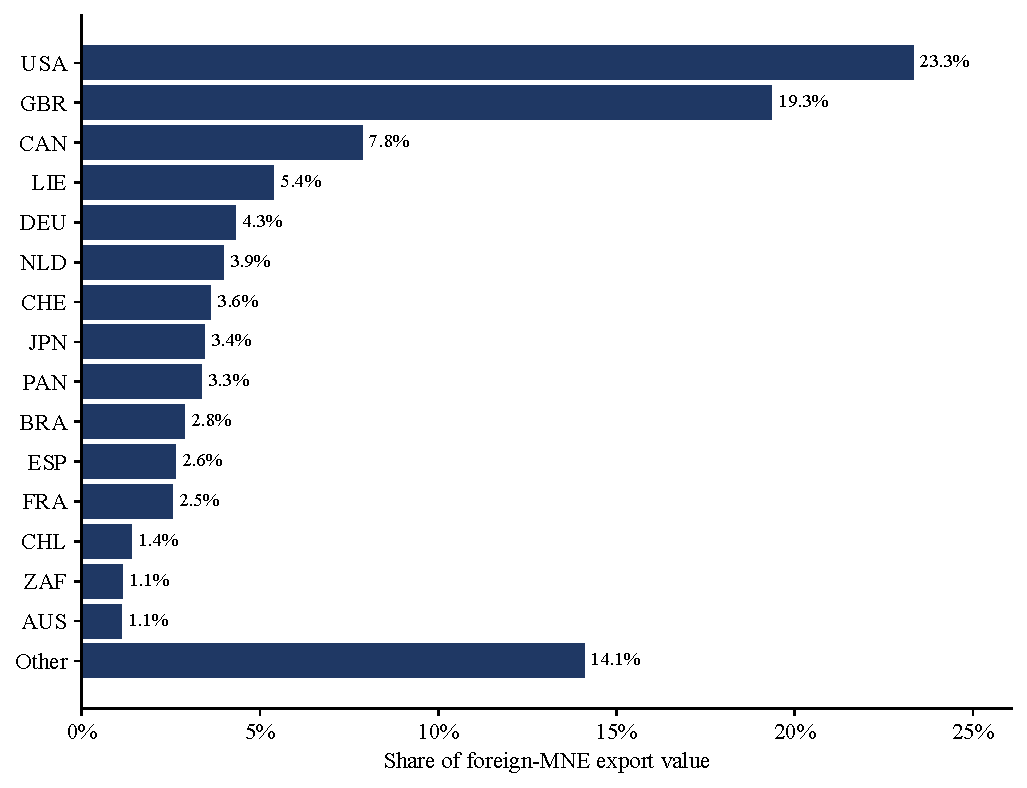
\includegraphics[width=0.78\textwidth,height=0.8\textheight,keepaspectratio]{figures/all/fig_wp1a_parent_share.pdf}%
  \caption{Foreign-Multinational Exports, by Parent Country}%
  \label{fig:f4_all}%
  \par\vspace{2pt}%
  \parbox{0.92\textwidth}{\footnotesize %
  \textit{Notes:} Percent of foreign-MNE export value, by country of the ultimate parent.\\[3pt]%
  \textit{Source:} Authors' calculations based on customs data matched to Orbis and Dun \& Bradstreet.}%
  \end{figure}
% ---- Table: Foreign-Multinational Exports, by Parent Country
\begin{table}[H]\centering\small%
  \caption{Foreign-Multinational Exports, by Parent Country}%
  \label{tab:f4n_all}%
  \adjustbox{max width=\textwidth, max totalheight=0.8\textheight}{\begin{tabular}{lrr}
\toprule
Parent country & Share (\%) & Value (US\$bn/yr) \\
\midrule
USA & 23.3 & 23.1 \\
GBR & 19.3 & 16.7 \\
CAN & 7.8 & 7.4 \\
LIE & 5.4 & 4.9 \\
DEU & 4.3 & 4.6 \\
NLD & 3.9 & 4.4 \\
CHE & 3.6 & 3.9 \\
JPN & 3.4 & 3.5 \\
PAN & 3.3 & 3.0 \\
BRA & 2.8 & 3.0 \\
ESP & 2.6 & 2.8 \\
FRA & 2.5 & 2.5 \\
CHL & 1.4 & 1.4 \\
ZAF & 1.1 & 1.0 \\
AUS & 1.1 & 1.1 \\
Other (150 countries) & 14.1 & 14.2 \\
\midrule
All foreign MNEs & 100.0 & 105.4 \\
\bottomrule
\end{tabular}
}%
  \par\vspace{3pt}%
  \begin{minipage}{0.95\textwidth}\footnotesize %
  \textit{Notes:} Percent of foreign-MNE export value, by country of the ultimate parent. Values are annual averages in US\$ billion.\\[3pt]%
  \textit{Source:} Authors' calculations based on customs data matched to Orbis and Dun \& Bradstreet.%
  \end{minipage}%
  \end{table}
% ---- Figure: Share of Total Exports, by Parent Country
\begin{figure}[H]\centering%
  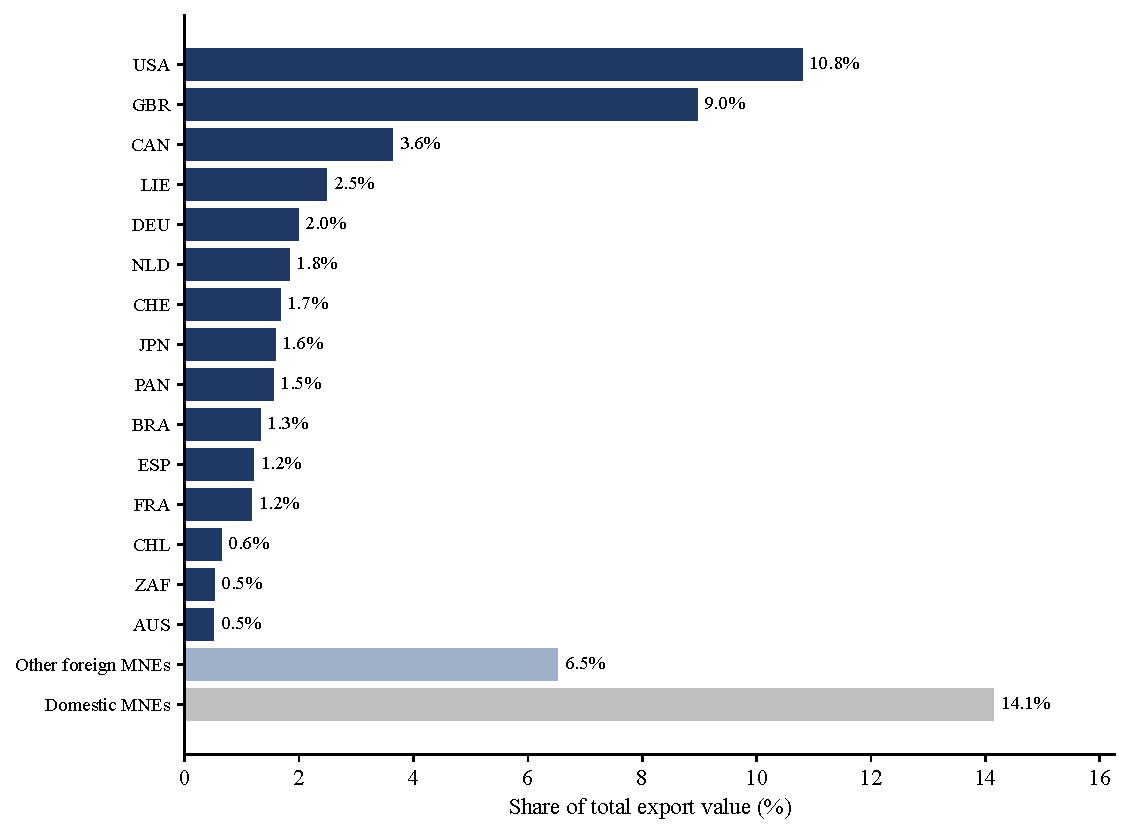
\includegraphics[width=0.85\textwidth,height=0.8\textheight,keepaspectratio]{figures/all/fig_wp1a_parent_share_total.pdf}%
  \caption{Share of Total Exports, by Parent Country}%
  \label{fig:f4t_all}%
  \par\vspace{2pt}%
  \parbox{0.92\textwidth}{\footnotesize %
  \textit{Notes:} Percent of total export value shipped by foreign MNEs of each parent country, other foreign MNEs and domestic MNEs; the remainder is local firms.\\[3pt]%
  \textit{Source:} Authors' calculations based on customs data matched to Orbis and Dun \& Bradstreet.}%
  \end{figure}
% ---- Table: Share of Total Exports, by Parent Country
\begin{table}[H]\centering\small%
  \caption{Share of Total Exports, by Parent Country}%
  \label{tab:f4tn_all}%
  \adjustbox{max width=\textwidth, max totalheight=0.8\textheight}{\begin{tabular}{lr}
\toprule
Exporter type / parent country & Share of total exports (\%) \\
\midrule
USA & 10.8 \\
GBR & 9.0 \\
CAN & 3.6 \\
LIE & 2.5 \\
DEU & 2.0 \\
NLD & 1.8 \\
CHE & 1.7 \\
JPN & 1.6 \\
PAN & 1.5 \\
BRA & 1.3 \\
ESP & 1.2 \\
FRA & 1.2 \\
CHL & 0.6 \\
ZAF & 0.5 \\
AUS & 0.5 \\
Other foreign MNEs & 6.5 \\
Domestic MNEs & 14.1 \\
\midrule
All MNEs & 60.5 \\
Local firms & 39.5 \\
\bottomrule
\end{tabular}
}%
  \par\vspace{3pt}%
  \begin{minipage}{0.95\textwidth}\footnotesize %
  \textit{Notes:} Percent of total export value, by type of exporter and parent country.\\[3pt]%
  \textit{Source:} Authors' calculations based on customs data matched to Orbis and Dun \& Bradstreet.%
  \end{minipage}%
  \end{table}

\subsection{Parent Region and Destination Region}
% ---- Table: Multinational Exports by Parent Region and Destination Region: Export Value
\begin{table}[H]\centering\small%
  \caption{Multinational Exports by Parent Region and Destination Region: Export Value}%
  \label{tab:reg_value_all}%
  \adjustbox{max width=\textwidth, max totalheight=0.8\textheight}{\begin{tabular}{lrrrrrrrr}
\toprule
Parent region / Destination region & Latin America & North America & Europe & Asia & Africa & Oceania & Rest of World & Total \\
\midrule
Latin America & 4.8 & 1.8 & 1.7 & 3.1 & 0.2 & 0.1 & 0.0 & 11.6 \\
North America & 9.7 & 7.3 & 5.9 & 7.0 & 0.6 & 0.0 & 0.0 & 30.5 \\
Europe & 13.8 & 5.5 & 8.4 & 16.3 & 1.5 & 0.5 & 0.1 & 46.0 \\
Asia & 3.7 & 1.3 & 0.8 & 1.1 & 0.1 & 0.0 & 0.0 & 7.0 \\
Africa & 0.2 & 0.1 & 0.3 & 0.7 & 0.0 & 0.0 & 0.0 & 1.3 \\
Oceania & 0.2 & 0.1 & 0.1 & 0.7 & 0.0 & 0.0 & 0.0 & 1.1 \\
Rest of World & 0.0 & 0.0 & 0.0 & 0.0 & 0.0 & 0.0 & 0.0 & 0.0 \\
Domestic MNEs & 7.6 & 9.4 & 3.3 & 7.8 & 0.8 & 0.2 & 0.1 & 29.1 \\
Local firms & 25.1 & 18.8 & 19.7 & 22.7 & 2.9 & 0.6 & 0.3 & 90.0 \\
\midrule
Total & 65.0 & 44.2 & 40.2 & 59.3 & 6.1 & 1.3 & 0.5 & 216.7 \\
\bottomrule
\end{tabular}
}%
  \par\vspace{3pt}%
  \begin{minipage}{0.95\textwidth}\footnotesize %
  \textit{Notes:} Values are annual averages in US\$ billion. Rows: region of the ultimate parent; columns: destination region.\\[3pt]%
  \textit{Source:} Authors' calculations based on customs data matched to Orbis and Dun \& Bradstreet.%
  \end{minipage}%
  \end{table}
% ---- Table: Multinational Exports by Parent Region and Destination Region: Row Percentages
\begin{table}[H]\centering\small%
  \caption{Multinational Exports by Parent Region and Destination Region: Row Percentages}%
  \label{tab:reg_rowpct_all}%
  \adjustbox{max width=\textwidth, max totalheight=0.8\textheight}{\begin{tabular}{lrrrrrrrr}
\toprule
Parent region / Destination region & Latin America & North America & Europe & Asia & Africa & Oceania & Rest of World & Total \\
\midrule
Latin America & 40.4 & 15.5 & 14.7 & 27.2 & 1.2 & 0.7 & 0.3 & 100.0 \\
North America & 31.3 & 23.6 & 20.0 & 23.1 & 1.7 & 0.1 & 0.1 & 100.0 \\
Europe & 28.0 & 11.7 & 17.8 & 38.4 & 2.9 & 1.0 & 0.1 & 100.0 \\
Asia & 51.0 & 18.7 & 11.7 & 17.0 & 1.1 & 0.2 & 0.3 & 100.0 \\
Africa & 10.9 & 6.6 & 26.9 & 53.2 & 2.2 & 0.0 & 0.2 & 100.0 \\
Oceania & 20.1 & 5.7 & 8.4 & 65.5 & 0.1 & 0.2 & 0.0 & 100.0 \\
Rest of World & 32.6 & 25.0 & 20.9 & 14.3 & 0.0 & 7.1 & 0.0 & 100.0 \\
Domestic MNEs & 25.9 & 32.9 & 11.1 & 27.0 & 2.3 & 0.5 & 0.3 & 100.0 \\
Local firms & 27.1 & 21.6 & 21.7 & 25.7 & 2.9 & 0.6 & 0.4 & 100.0 \\
\bottomrule
\end{tabular}
}%
  \par\vspace{3pt}%
  \begin{minipage}{0.95\textwidth}\footnotesize %
  \textit{Notes:} Percent of each group's exports, by destination region (rows add to 100). Domestic MNEs and local firms are shown for comparison.\\[3pt]%
  \textit{Source:} Authors' calculations based on customs data matched to Orbis and Dun \& Bradstreet.%
  \end{minipage}%
  \end{table}
% ---- Table: Multinational Exports by Parent Region and Destination Region: Column Percentages
\begin{table}[H]\centering\small%
  \caption{Multinational Exports by Parent Region and Destination Region: Column Percentages}%
  \label{tab:reg_colpct_all}%
  \adjustbox{max width=\textwidth, max totalheight=0.8\textheight}{\begin{tabular}{lrrrrrrr}
\toprule
Parent region / Destination region & Latin America & North America & Europe & Asia & Africa & Oceania & Rest of World \\
\midrule
Latin America & 7.4 & 3.9 & 4.3 & 5.1 & 2.6 & 6.2 & 6.3 \\
North America & 14.9 & 15.7 & 15.0 & 11.2 & 9.8 & 1.8 & 4.9 \\
Europe & 20.4 & 11.9 & 20.5 & 28.7 & 25.0 & 37.1 & 10.3 \\
Asia & 5.2 & 2.7 & 1.9 & 1.8 & 1.3 & 0.9 & 3.2 \\
Africa & 0.2 & 0.2 & 0.9 & 1.1 & 0.5 & 0.0 & 0.4 \\
Oceania & 0.3 & 0.1 & 0.2 & 1.1 & 0.0 & 0.1 & 0.0 \\
Rest of World & 0.0 & 0.0 & 0.0 & 0.0 & 0.0 & 0.1 & 0.0 \\
Domestic MNEs & 13.1 & 23.1 & 8.9 & 13.9 & 13.5 & 12.2 & 15.0 \\
Local firms & 38.3 & 42.4 & 48.3 & 37.1 & 47.3 & 41.4 & 59.9 \\
\midrule
Total & 100.0 & 100.0 & 100.0 & 100.0 & 100.0 & 100.0 & 100.0 \\
\bottomrule
\end{tabular}
}%
  \par\vspace{3pt}%
  \begin{minipage}{0.95\textwidth}\footnotesize %
  \textit{Notes:} Percent of the exports reaching each destination region, by parent region (columns add to 100).\\[3pt]%
  \textit{Source:} Authors' calculations based on customs data matched to Orbis and Dun \& Bradstreet.%
  \end{minipage}%
  \end{table}
% ---- Figure: Multinational Exports by Parent Region and Destination Region
\begin{figure}[H]\centering%
  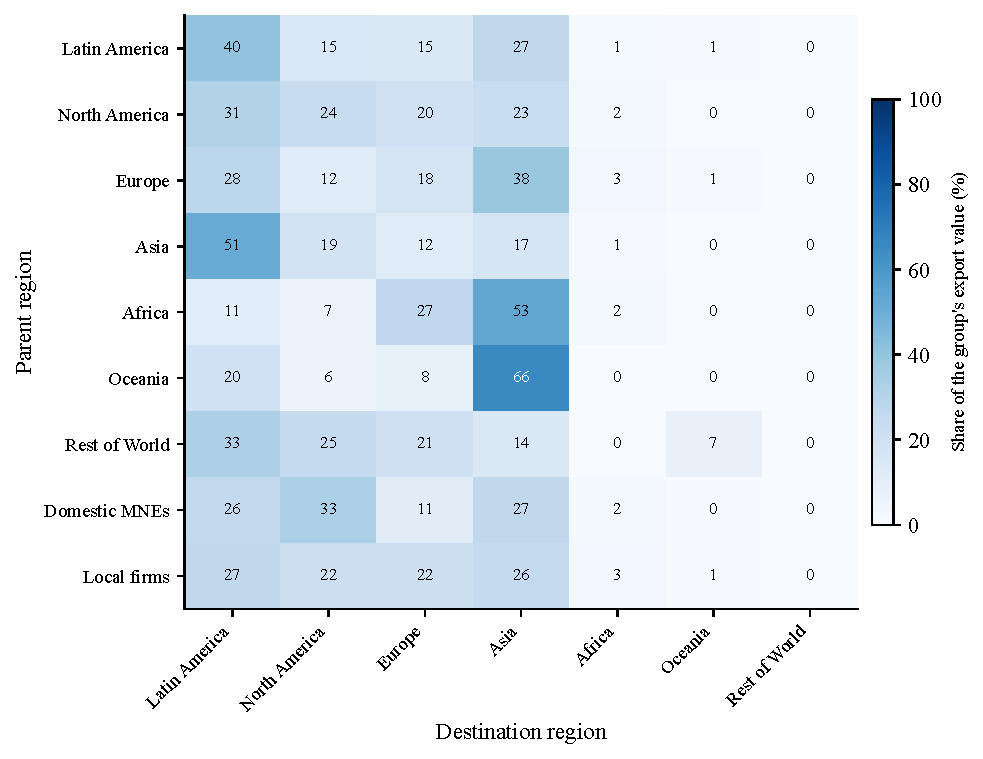
\includegraphics[width=0.9\textwidth,height=0.8\textheight,keepaspectratio]{figures/all/fig_wp1d_heatmap_region_rowpct.pdf}%
  \caption{Multinational Exports by Parent Region and Destination Region}%
  \label{fig:reg_hm_all}%
  \par\vspace{2pt}%
  \parbox{0.92\textwidth}{\footnotesize %
  \textit{Notes:} Percent of each group's exports, by destination region (rows add to 100).\\[3pt]%
  \textit{Source:} Authors' calculations based on customs data matched to Orbis and Dun \& Bradstreet.}%
  \end{figure}
% ---- Table: Foreign-Multinational Exports by Exporting Country and Destination Region
\begin{table}[H]\centering\small%
  \caption{Foreign-Multinational Exports by Exporting Country and Destination Region}%
  \label{tab:odr_f_all}%
  \adjustbox{max width=\textwidth, max totalheight=0.8\textheight}{\begin{tabular}{lrrrrrrrr}
\toprule
Origin \ Destination region & Latin America & North America & Europe & Asia & Africa & Oceania & Rest of World & Total \\
\midrule
ARG & 45.5 & 9.0 & 15.5 & 23.0 & 6.2 & 0.8 & 0.0 & 32.5 \\
CHL & 13.1 & 11.6 & 13.3 & 60.5 & 0.3 & 1.2 & 0.0 & 16.4 \\
COL & 40.7 & 19.7 & 25.4 & 12.6 & 0.5 & 0.3 & 0.9 & 15.5 \\
CRI & 33.0 & 40.7 & 16.2 & 9.8 & 0.1 & 0.1 & 0.0 & 6.3 \\
DOM & 20.3 & 59.3 & 9.4 & 10.5 & 0.2 & 0.2 & 0.1 & 5.9 \\
PER & 15.4 & 12.9 & 25.3 & 44.9 & 1.0 & 0.4 & 0.0 & 18.3 \\
PRY & 79.4 & 1.3 & 11.6 & 6.6 & 1.1 & 0.0 & 0.0 & 4.4 \\
SLV & 46.8 & 48.1 & 4.3 & 0.6 & 0.1 & 0.1 & 0.0 & 2.4 \\
URY & 39.1 & 7.7 & 20.5 & 28.0 & 3.0 & 0.1 & 1.6 & 3.7 \\
\bottomrule
\end{tabular}
}%
  \par\vspace{3pt}%
  \begin{minipage}{0.95\textwidth}\footnotesize %
  \textit{Notes:} Percent of each country's foreign-MNE exports, by destination region (rows add to 100). Last column: foreign-MNE exports. Values are annual averages in US\$ billion.\\[3pt]%
  \textit{Source:} Authors' calculations based on customs data matched to Orbis and Dun \& Bradstreet.%
  \end{minipage}%
  \end{table}
% ---- Table: Local-Firm Exports by Exporting Country and Destination Region
\begin{table}[H]\centering\small%
  \caption{Local-Firm Exports by Exporting Country and Destination Region}%
  \label{tab:odr_l_all}%
  \adjustbox{max width=\textwidth, max totalheight=0.8\textheight}{\begin{tabular}{lrrrrrrrr}
\toprule
Origin \ Destination region & Latin America & North America & Europe & Asia & Africa & Oceania & Rest of World & Total \\
\midrule
ARG & 32.2 & 8.3 & 21.4 & 28.5 & 8.4 & 1.3 & 0.0 & 29.0 \\
CHL & 15.5 & 18.8 & 20.4 & 44.3 & 0.6 & 0.5 & 0.0 & 13.2 \\
COL & 32.2 & 32.8 & 23.5 & 8.5 & 0.8 & 0.3 & 1.9 & 11.2 \\
CRI & 32.1 & 35.4 & 26.3 & 5.4 & 0.3 & 0.5 & 0.0 & 3.8 \\
DOM & 31.9 & 46.8 & 15.7 & 4.6 & 0.6 & 0.0 & 0.3 & 2.6 \\
PER & 18.3 & 28.0 & 24.6 & 28.1 & 0.3 & 0.4 & 0.2 & 22.1 \\
PRY & 64.6 & 3.6 & 20.0 & 10.6 & 1.1 & 0.0 & 0.0 & 2.7 \\
SLV & 44.9 & 46.3 & 4.6 & 3.7 & 0.1 & 0.3 & 0.1 & 2.6 \\
URY & 38.7 & 5.2 & 21.6 & 26.0 & 7.3 & 0.1 & 1.3 & 2.6 \\
\bottomrule
\end{tabular}
}%
  \par\vspace{3pt}%
  \begin{minipage}{0.95\textwidth}\footnotesize %
  \textit{Notes:} Percent of each country's exports by local firms, by destination region (rows add to 100). Last column: local-firm exports. Values are annual averages in US\$ billion.\\[3pt]%
  \textit{Source:} Authors' calculations based on customs data matched to Orbis and Dun \& Bradstreet.%
  \end{minipage}%
  \end{table}

\subsection{Parent Country and Destination Country}
% ---- Table: Foreign-Multinational Exports by Parent Country and Destination: Export Value
\begin{table}[H]\centering\small%
  \caption{Foreign-Multinational Exports by Parent Country and Destination: Export Value}%
  \label{tab:cty_value_all}%
  \adjustbox{max width=\textwidth, max totalheight=0.8\textheight}{\begin{tabular}{lrrrrrrrrrrrr}
\toprule
Parent / Destination & CHN & USA & BRA & JPN & ESP & CHL & KOR & CAN & NLD & ARG & Other destinations & Total \\
\midrule
USA & 2.4 & 5.0 & 1.9 & 0.9 & 0.9 & 0.7 & 0.5 & 0.1 & 0.8 & 1.3 & 8.7 & 23.1 \\
GBR & 5.9 & 0.9 & 0.7 & 1.1 & 0.5 & 0.6 & 1.1 & 0.6 & 0.5 & 0.0 & 4.7 & 16.7 \\
CAN & 0.8 & 0.5 & 0.3 & 0.3 & 0.2 & 0.0 & 0.1 & 1.7 & 0.1 & 0.0 & 3.4 & 7.4 \\
LIE & 1.1 & 0.2 & 0.2 & 0.7 & 0.2 & 0.2 & 0.2 & 0.0 & 0.1 & 0.0 & 2.0 & 4.9 \\
DEU & 0.0 & 0.7 & 1.5 & 0.0 & 0.1 & 0.1 & 0.0 & 0.0 & 0.0 & 0.0 & 1.9 & 4.6 \\
NLD & 0.4 & 0.2 & 1.2 & 0.0 & 0.0 & 0.2 & 0.1 & 0.0 & 0.1 & 0.1 & 2.1 & 4.4 \\
CHE & 0.2 & 0.2 & 0.3 & 0.0 & 0.1 & 0.1 & 0.0 & 0.0 & 0.1 & 0.0 & 2.8 & 3.9 \\
JPN & 0.1 & 0.3 & 1.7 & 0.2 & 0.0 & 0.1 & 0.0 & 0.0 & 0.0 & 0.1 & 1.0 & 3.5 \\
PAN & 1.0 & 0.3 & 0.0 & 0.1 & 0.1 & 0.0 & 0.2 & 0.0 & 0.1 & 0.0 & 1.2 & 3.0 \\
BRA & 0.4 & 0.4 & 0.6 & 0.0 & 0.0 & 0.1 & 0.0 & 0.0 & 0.1 & 0.1 & 1.3 & 3.0 \\
Other parents & 2.2 & 4.5 & 2.8 & 0.5 & 0.8 & 1.0 & 0.3 & 0.4 & 0.5 & 0.9 & 9.1 & 23.0 \\
\midrule
Total & 14.6 & 13.1 & 11.2 & 4.0 & 3.0 & 3.1 & 2.5 & 2.9 & 2.3 & 2.5 & 38.3 & 97.6 \\
\bottomrule
\end{tabular}
}%
  \par\vspace{3pt}%
  \begin{minipage}{0.95\textwidth}\footnotesize %
  \textit{Notes:} Values are annual averages in US\$ billion. Ten largest parent countries and ten largest destinations by foreign-MNE export value.\\[3pt]%
  \textit{Source:} Authors' calculations based on customs data matched to Orbis and Dun \& Bradstreet.%
  \end{minipage}%
  \end{table}
% ---- Table: Foreign-Multinational Exports by Parent Country and Destination: Row Percentages
\begin{table}[H]\centering\small%
  \caption{Foreign-Multinational Exports by Parent Country and Destination: Row Percentages}%
  \label{tab:cty_rowpct_all}%
  \adjustbox{max width=\textwidth, max totalheight=0.8\textheight}{\begin{tabular}{lrrrrrrrrrrrr}
\toprule
Parent / Destination & CHN & USA & BRA & JPN & ESP & CHL & KOR & CAN & NLD & ARG & Other destinations & Total \\
\midrule
USA & 10.1 & 22.3 & 7.8 & 3.8 & 4.0 & 2.9 & 2.1 & 0.5 & 3.5 & 4.9 & 38.2 & 100.0 \\
GBR & 36.5 & 5.6 & 3.9 & 7.1 & 3.0 & 3.4 & 6.5 & 3.3 & 3.2 & 0.2 & 27.3 & 100.0 \\
CAN & 12.8 & 6.6 & 4.2 & 5.3 & 3.1 & 0.5 & 1.9 & 19.5 & 0.9 & 0.2 & 45.0 & 100.0 \\
LIE & 24.9 & 3.7 & 3.7 & 18.7 & 3.5 & 2.5 & 5.4 & 0.0 & 1.8 & 0.0 & 35.6 & 100.0 \\
DEU & 1.0 & 14.8 & 31.9 & 1.1 & 1.7 & 3.1 & 0.6 & 1.1 & 1.0 & 0.9 & 42.8 & 100.0 \\
NLD & 9.2 & 3.8 & 26.9 & 0.4 & 1.0 & 3.6 & 1.1 & 0.2 & 2.2 & 3.1 & 48.4 & 100.0 \\
CHE & 6.2 & 5.0 & 6.8 & 0.5 & 2.9 & 3.5 & 0.8 & 0.4 & 2.0 & 0.5 & 71.4 & 100.0 \\
JPN & 2.4 & 8.7 & 45.0 & 8.9 & 0.4 & 1.4 & 0.4 & 0.5 & 0.9 & 1.9 & 29.5 & 100.0 \\
PAN & 35.0 & 9.5 & 1.2 & 1.8 & 1.7 & 1.1 & 6.2 & 0.6 & 2.0 & 0.2 & 40.7 & 100.0 \\
BRA & 12.9 & 14.1 & 18.6 & 1.6 & 0.6 & 3.1 & 0.6 & 0.6 & 2.1 & 2.3 & 43.4 & 100.0 \\
Other parents & 9.5 & 19.5 & 11.7 & 2.2 & 3.7 & 4.0 & 1.6 & 1.6 & 2.1 & 3.7 & 40.3 & 100.0 \\
\bottomrule
\end{tabular}
}%
  \par\vspace{3pt}%
  \begin{minipage}{0.95\textwidth}\footnotesize %
  \textit{Notes:} Percent of each parent country's exports, by destination (rows add to 100). Ten largest parent countries and destinations.\\[3pt]%
  \textit{Source:} Authors' calculations based on customs data matched to Orbis and Dun \& Bradstreet.%
  \end{minipage}%
  \end{table}
% ---- Table: Foreign-Multinational Exports by Parent Country and Destination: Column Percentages
\begin{table}[H]\centering\small%
  \caption{Foreign-Multinational Exports by Parent Country and Destination: Column Percentages}%
  \label{tab:cty_colpct_all}%
  \adjustbox{max width=\textwidth, max totalheight=0.8\textheight}{\begin{tabular}{lrrrrrrrrrrr}
\toprule
Parent / Destination & CHN & USA & BRA & JPN & ESP & CHL & KOR & CAN & NLD & ARG & Other destinations \\
\midrule
USA & 14.6 & 38.7 & 17.2 & 18.8 & 30.1 & 22.5 & 17.0 & 4.1 & 33.0 & 48.1 & 23.0 \\
GBR & 43.7 & 8.1 & 7.2 & 29.3 & 18.8 & 21.8 & 43.5 & 22.8 & 25.7 & 1.5 & 13.7 \\
CAN & 6.2 & 3.8 & 3.1 & 9.0 & 7.8 & 1.4 & 5.1 & 55.1 & 3.0 & 0.8 & 9.1 \\
LIE & 8.3 & 1.5 & 1.9 & 21.5 & 6.1 & 4.6 & 10.1 & 0.1 & 4.0 & 0.1 & 4.9 \\
DEU & 0.3 & 4.7 & 13.0 & 1.0 & 2.4 & 4.5 & 0.9 & 1.7 & 1.8 & 1.6 & 4.7 \\
NLD & 2.3 & 1.1 & 10.1 & 0.3 & 1.3 & 4.7 & 1.6 & 0.2 & 3.5 & 5.2 & 4.9 \\
CHE & 1.4 & 1.3 & 2.3 & 0.4 & 3.3 & 4.3 & 1.0 & 0.6 & 2.9 & 0.8 & 6.6 \\
JPN & 0.5 & 2.2 & 14.6 & 6.5 & 0.5 & 1.6 & 0.4 & 0.6 & 1.2 & 2.7 & 2.6 \\
PAN & 7.2 & 2.4 & 0.4 & 1.3 & 1.8 & 1.2 & 7.2 & 0.8 & 2.8 & 0.2 & 3.5 \\
BRA & 2.3 & 3.0 & 5.0 & 1.0 & 0.6 & 2.9 & 0.6 & 0.6 & 2.5 & 2.8 & 3.2 \\
Other parents & 13.4 & 33.1 & 25.3 & 10.9 & 27.3 & 30.4 & 12.6 & 13.4 & 19.6 & 36.0 & 23.7 \\
\midrule
Total & 100.0 & 100.0 & 100.0 & 100.0 & 100.0 & 100.0 & 100.0 & 100.0 & 100.0 & 100.0 & 100.0 \\
\bottomrule
\end{tabular}
}%
  \par\vspace{3pt}%
  \begin{minipage}{0.95\textwidth}\footnotesize %
  \textit{Notes:} Percent of the foreign-MNE exports reaching each destination, by parent country (columns add to 100). Ten largest parent countries and destinations.\\[3pt]%
  \textit{Source:} Authors' calculations based on customs data matched to Orbis and Dun \& Bradstreet.%
  \end{minipage}%
  \end{table}
% ---- Figure: Destination of Foreign-Multinational Exports: Fifteen Largest Parent Countries and Destinations
\begin{figure}[H]\centering%
  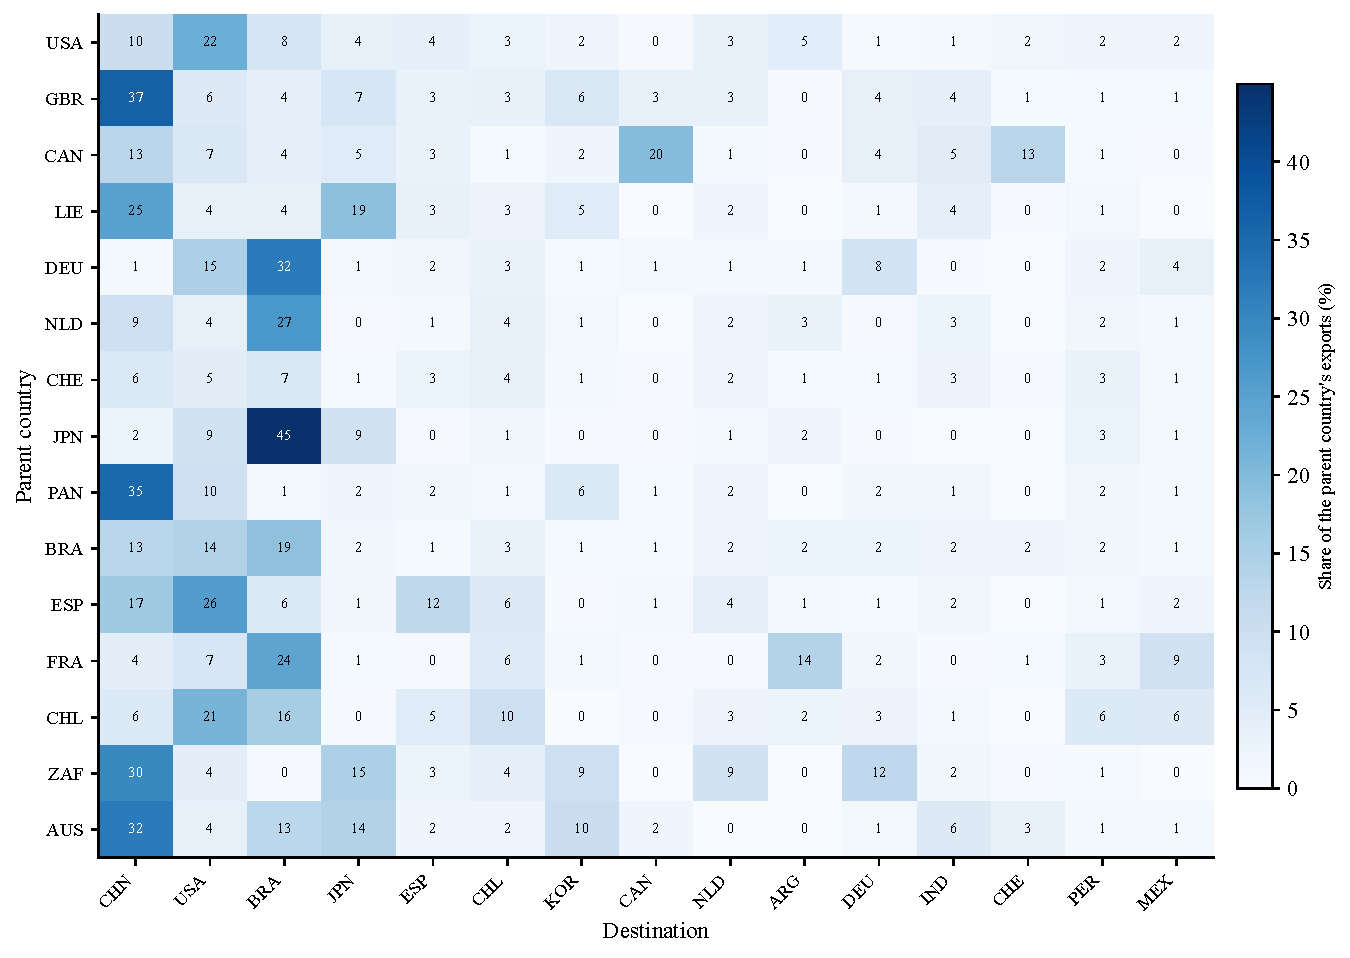
\includegraphics[width=1.0\textwidth,height=0.8\textheight,keepaspectratio]{figures/all/fig_wp1d_heatmap_country_rowpct.pdf}%
  \caption{Destination of Foreign-Multinational Exports: Fifteen Largest Parent Countries and Destinations}%
  \label{fig:hm_row_all}%
  \par\vspace{2pt}%
  \parbox{0.92\textwidth}{\footnotesize %
  \textit{Notes:} Percent of each parent country's exports going to each destination (rows add to 100 including other destinations).\\[3pt]%
  \textit{Source:} Authors' calculations based on customs data matched to Orbis and Dun \& Bradstreet.}%
  \end{figure}
% ---- Figure: Foreign-Multinational Exports by Parent Country and Destination: Share of the Total
\begin{figure}[H]\centering%
  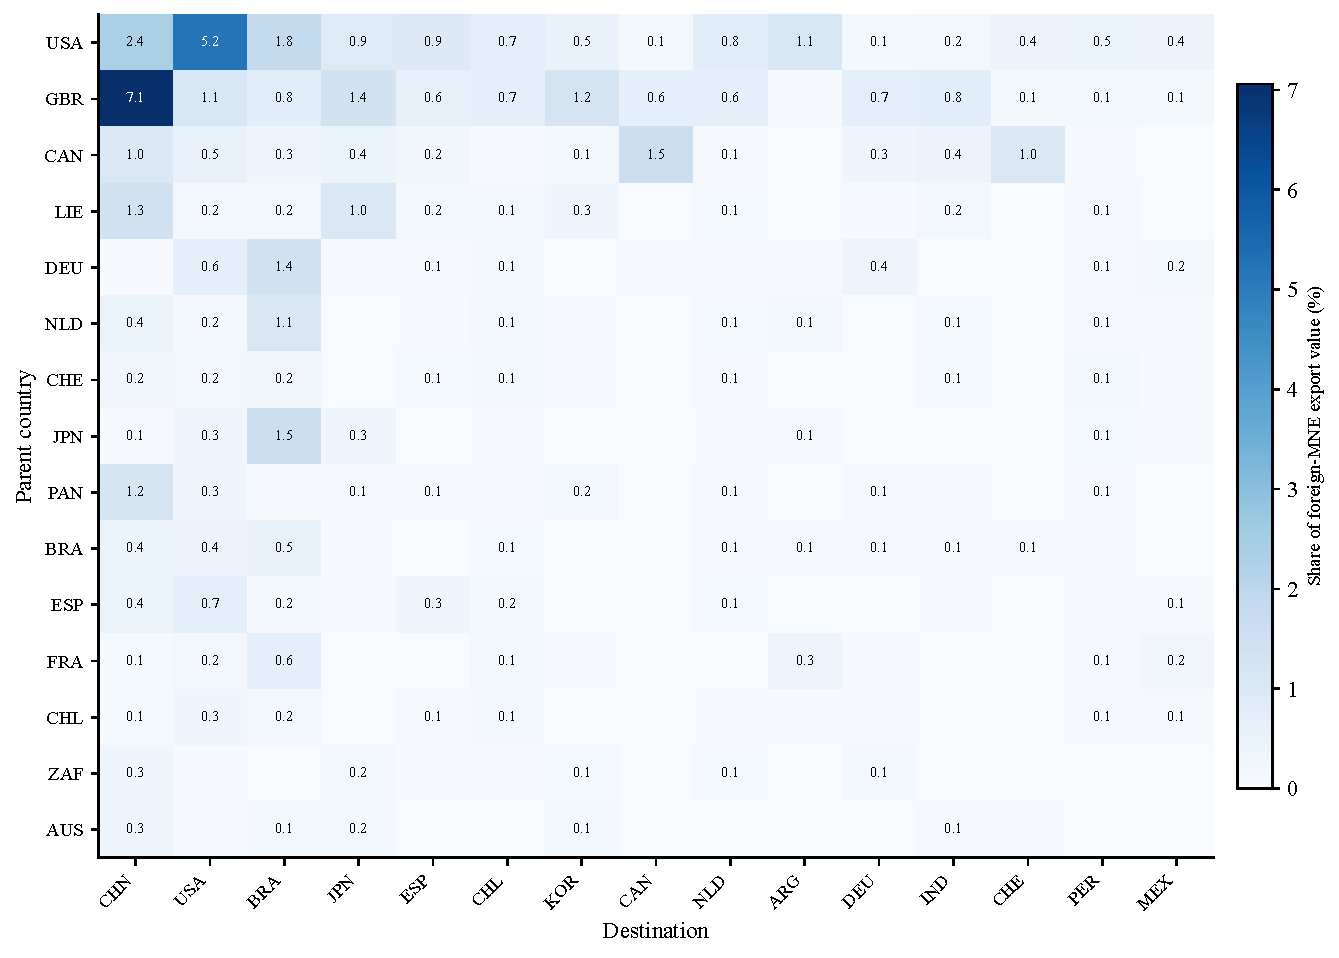
\includegraphics[width=1.0\textwidth,height=0.8\textheight,keepaspectratio]{figures/all/fig_wp1d_heatmap_country_cellpct.pdf}%
  \caption{Foreign-Multinational Exports by Parent Country and Destination: Share of the Total}%
  \label{fig:hm_cell_all}%
  \par\vspace{2pt}%
  \parbox{0.92\textwidth}{\footnotesize %
  \textit{Notes:} Percent of all foreign-MNE export value in each parent country and destination pair; fifteen largest parent countries and destinations.\\[3pt]%
  \textit{Source:} Authors' calculations based on customs data matched to Orbis and Dun \& Bradstreet.}%
  \end{figure}

\subsection{Exports to the Parent Country}
% ---- Figure: Share of Foreign-Multinational Exports Shipped to the Parent Country
\begin{figure}[H]\centering%
  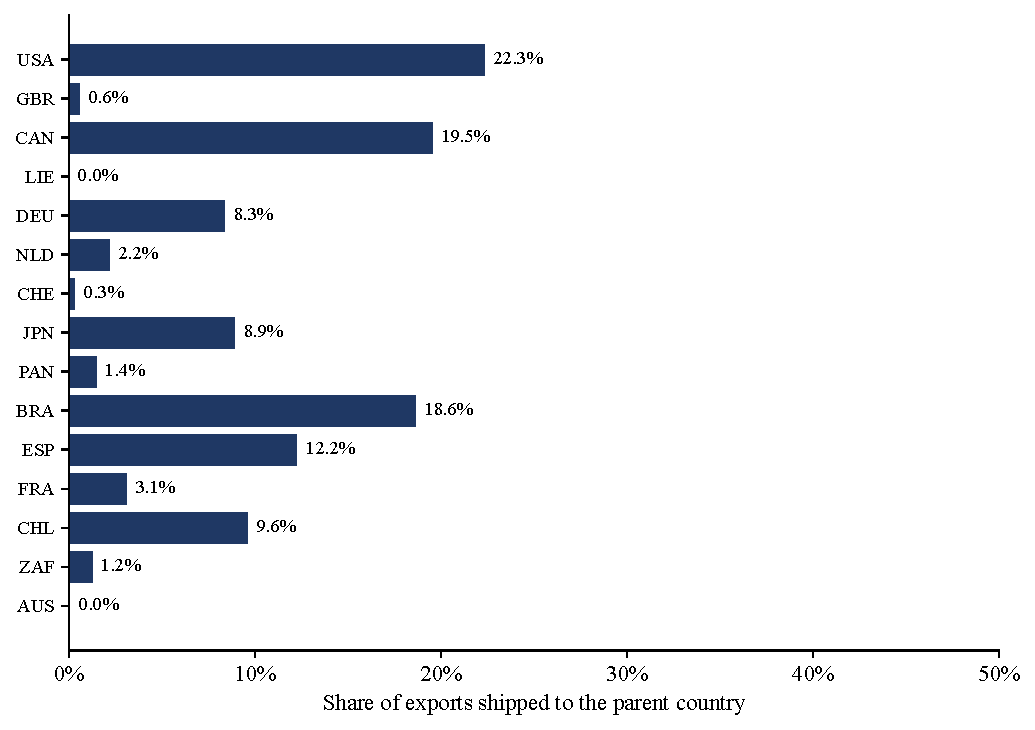
\includegraphics[width=0.85\textwidth,height=0.8\textheight,keepaspectratio]{figures/all/fig_wp1d_home_share_by_parent.pdf}%
  \caption{Share of Foreign-Multinational Exports Shipped to the Parent Country}%
  \label{fig:home_all}%
  \par\vspace{2pt}%
  \parbox{0.92\textwidth}{\footnotesize %
  \textit{Notes:} Percent of each parent country's exports shipped to that same country.\\[3pt]%
  \textit{Source:} Authors' calculations based on customs data matched to Orbis and Dun \& Bradstreet.}%
  \end{figure}
% ---- Table: Foreign-Multinational Exports to the Parent Countries, by Parent Country
\begin{table}[H]\centering\small%
  \caption{Foreign-Multinational Exports to the Parent Countries, by Parent Country}%
  \label{tab:pxp_all}%
  \adjustbox{max width=\textwidth, max totalheight=0.8\textheight}{\begin{tabular}{lrrrrrrrrrrrr}
\toprule
Parent / Destination & USA & GBR & CAN & LIE & DEU & NLD & CHE & JPN & PAN & BRA & Other destinations & Total \\
\midrule
USA & 22.3 & 1.0 & 0.5 & 0.0 & 0.6 & 3.5 & 1.7 & 3.8 & 2.7 & 7.8 & 56.2 & 100.0 \\
GBR & 5.6 & 0.6 & 3.3 & 0.0 & 3.6 & 3.2 & 0.6 & 7.1 & 0.2 & 3.9 & 71.8 & 100.0 \\
CAN & 6.6 & 2.6 & 19.5 & 0.0 & 3.5 & 0.9 & 12.9 & 5.3 & 2.6 & 4.2 & 41.8 & 100.0 \\
LIE & 3.7 & 0.4 & 0.0 & 0.0 & 0.9 & 1.8 & 0.2 & 18.7 & 0.1 & 3.7 & 70.5 & 100.0 \\
DEU & 14.8 & 0.3 & 1.1 & 0.0 & 8.3 & 1.0 & 0.0 & 1.1 & 0.8 & 31.9 & 40.6 & 100.0 \\
NLD & 3.8 & 0.5 & 0.2 & 0.0 & 0.4 & 2.2 & 0.0 & 0.4 & 0.4 & 26.9 & 65.2 & 100.0 \\
CHE & 5.0 & 1.0 & 0.4 & 0.0 & 0.7 & 2.0 & 0.3 & 0.5 & 1.7 & 6.8 & 81.6 & 100.0 \\
JPN & 8.7 & 0.3 & 0.5 & 0.0 & 0.2 & 0.9 & 0.0 & 8.9 & 1.0 & 45.0 & 34.5 & 100.0 \\
PAN & 9.5 & 0.8 & 0.6 & 0.0 & 1.7 & 2.0 & 0.2 & 1.8 & 1.4 & 1.2 & 80.7 & 100.0 \\
BRA & 14.1 & 0.5 & 0.6 & 0.0 & 2.3 & 2.1 & 2.2 & 1.6 & 0.6 & 18.6 & 57.4 & 100.0 \\
Other parents & 19.5 & 0.9 & 1.6 & 0.0 & 2.2 & 2.1 & 1.2 & 2.2 & 1.7 & 11.7 & 56.8 & 100.0 \\
\bottomrule
\end{tabular}
}%
  \par\vspace{3pt}%
  \begin{minipage}{0.95\textwidth}\footnotesize %
  \textit{Notes:} Percent of each parent country's exports, by destination (rows add to 100). Destinations are the ten largest parent countries; the diagonal is the share shipped to the parent's own country.\\[3pt]%
  \textit{Source:} Authors' calculations based on customs data matched to Orbis and Dun \& Bradstreet.%
  \end{minipage}%
  \end{table}
% ---- Figure: Share of Foreign-Multinational Exports Shipped to the Parent Jurisdiction, Consolidated Parents
\begin{figure}[H]\centering%
  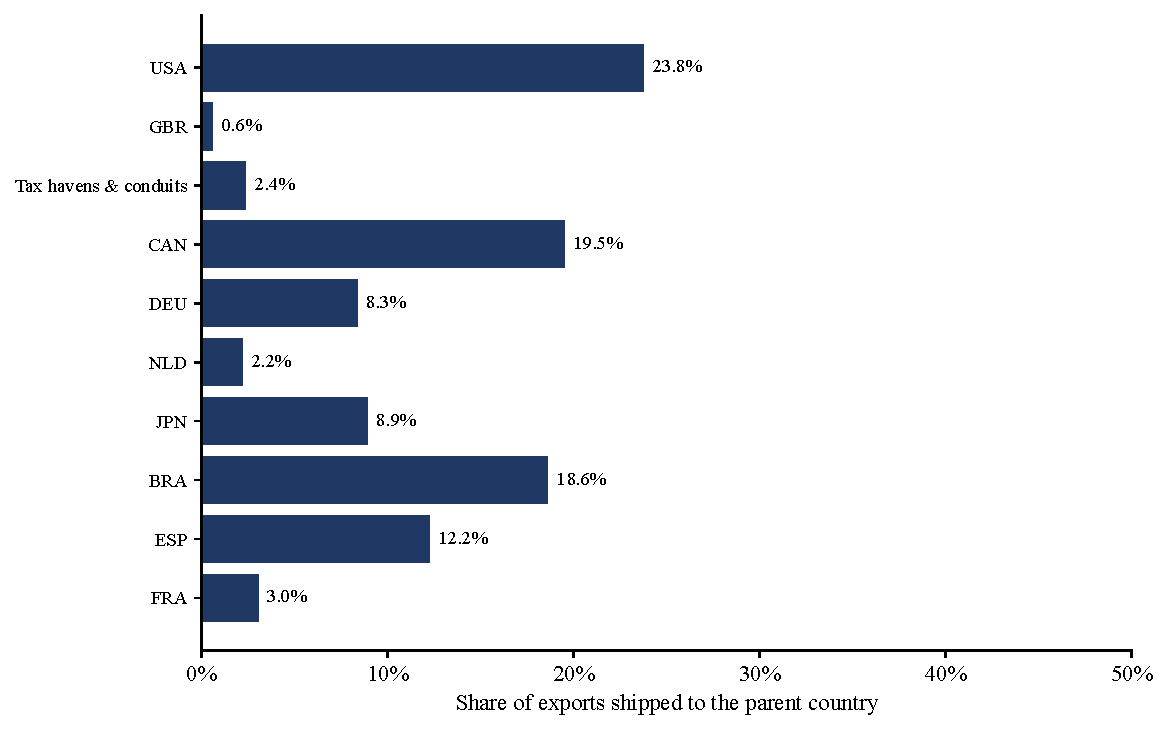
\includegraphics[width=0.85\textwidth,height=0.8\textheight,keepaspectratio]{figures/all/fig_wp1d_home_share_by_parent_consolidated.pdf}%
  \caption{Share of Foreign-Multinational Exports Shipped to the Parent Jurisdiction, Consolidated Parents}%
  \label{fig:homec_all}%
  \par\vspace{2pt}%
  \parbox{0.92\textwidth}{\footnotesize %
  \textit{Notes:} Percent of each parent's exports shipped to its own jurisdiction. Dependencies are assigned to their sovereign state and tax havens and conduit jurisdictions are pooled.\\[3pt]%
  \textit{Source:} Authors' calculations based on customs data matched to Orbis and Dun \& Bradstreet.}%
  \end{figure}
% ---- Table: Share of Foreign-Multinational Exports Shipped to the Parent Jurisdiction, Consolidated Parents
\begin{table}[H]\centering\small%
  \caption{Share of Foreign-Multinational Exports Shipped to the Parent Jurisdiction, Consolidated Parents}%
  \label{tab:homec_t_all}%
  \adjustbox{max width=\textwidth, max totalheight=0.8\textheight}{\begin{tabular}{lrr}
\toprule
Consolidated parent & Home share (\%) & Exports (US\$bn/yr) \\
\midrule
USA & 23.8 & 23.1 \\
GBR & 0.6 & 18.4 \\
Tax havens \& conduits & 2.4 & 14.7 \\
CAN & 19.5 & 7.4 \\
DEU & 8.3 & 4.6 \\
NLD & 2.2 & 4.4 \\
JPN & 8.9 & 3.5 \\
BRA & 18.6 & 3.0 \\
ESP & 12.2 & 2.8 \\
FRA & 3.0 & 2.6 \\
\bottomrule
\end{tabular}
}%
  \par\vspace{3pt}%
  \begin{minipage}{0.95\textwidth}\footnotesize %
  \textit{Notes:} Home share: percent of the parent's exports shipped to its own jurisdiction. Values are annual averages in US\$ billion.\\[3pt]%
  \textit{Source:} Authors' calculations based on customs data matched to Orbis and Dun \& Bradstreet.%
  \end{minipage}%
  \end{table}
% ---- Figure: Share of Foreign-Multinational Exports Shipped to the Parent Jurisdiction
\begin{figure}[H]\centering%
  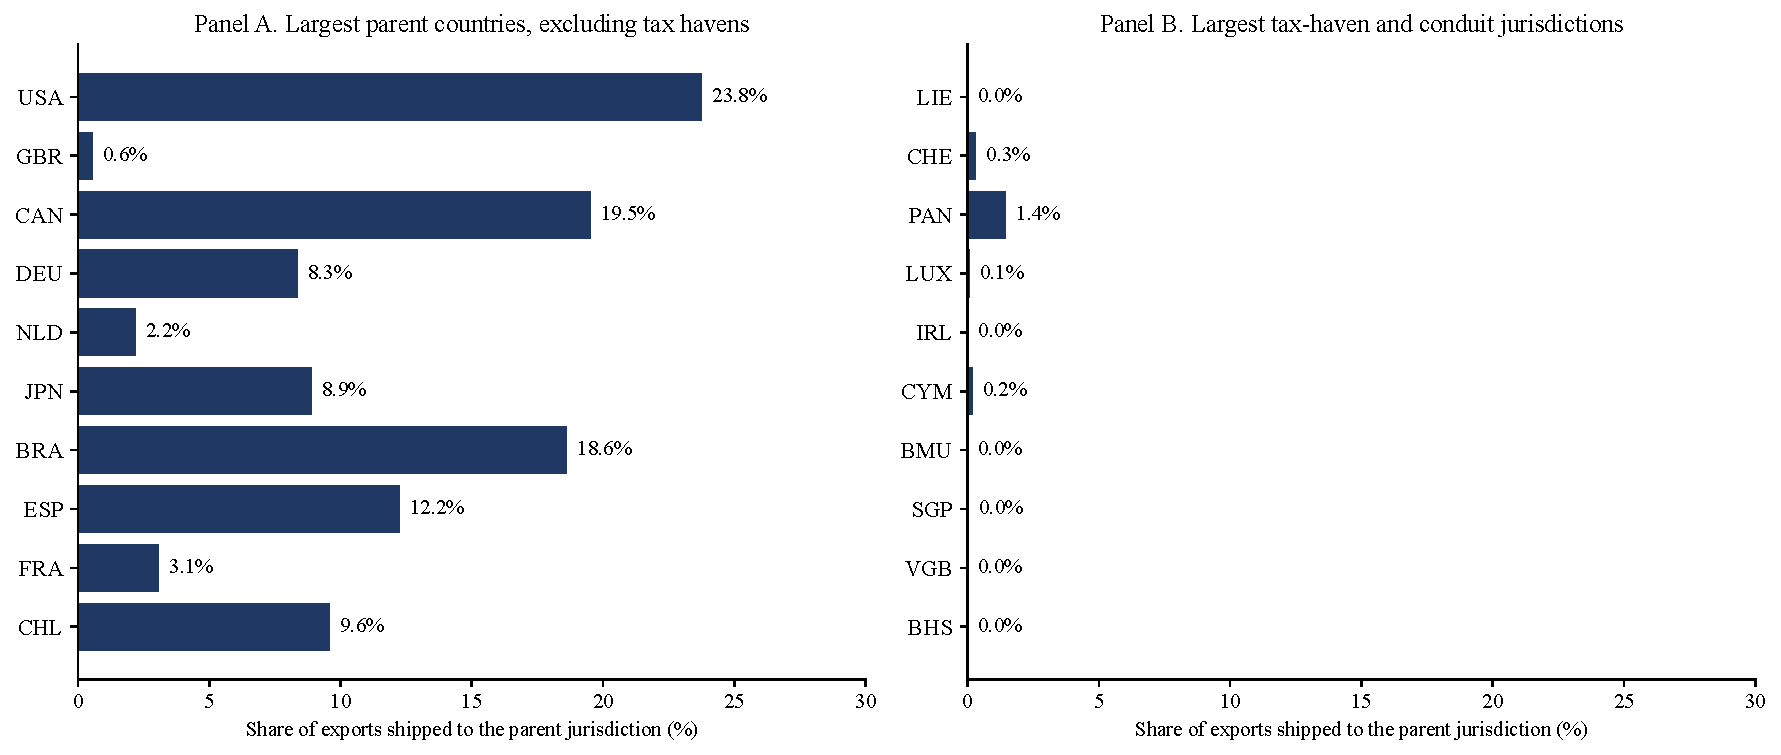
\includegraphics[width=1.0\textwidth,height=0.8\textheight,keepaspectratio]{figures/all/fig_wp1d_home_share_haven_panels.pdf}%
  \caption{Share of Foreign-Multinational Exports Shipped to the Parent Jurisdiction}%
  \label{fig:homeh_all}%
  \par\vspace{2pt}%
  \parbox{0.92\textwidth}{\footnotesize %
  \textit{Notes:} Percent of each parent jurisdiction's exports shipped to that same jurisdiction. Panel A: largest parent countries, excluding tax havens; dependencies are assigned to their sovereign state. Panel B: largest tax-haven and conduit jurisdictions.\\[3pt]%
  \textit{Source:} Authors' calculations based on customs data matched to Orbis and Dun \& Bradstreet.}%
  \end{figure}
% ---- Table: Share of Foreign-Multinational Exports Shipped to the Parent Jurisdiction
\begin{table}[H]\centering\small%
  \caption{Share of Foreign-Multinational Exports Shipped to the Parent Jurisdiction}%
  \label{tab:homeh_t_all}%
  \adjustbox{max width=\textwidth, max totalheight=0.8\textheight}{\begin{tabular}{llrr}
\toprule
Panel & Parent & Home share (\%) & Exports (US\$bn/yr) \\
\midrule
Panel A & USA & 23.8 & 23.1 \\
Panel A & GBR & 0.6 & 16.7 \\
Panel A & CAN & 19.5 & 7.4 \\
Panel A & DEU & 8.3 & 4.6 \\
Panel A & NLD & 2.2 & 4.4 \\
Panel A & JPN & 8.9 & 3.5 \\
Panel A & BRA & 18.6 & 3.0 \\
Panel A & ESP & 12.2 & 2.8 \\
Panel A & FRA & 3.1 & 2.5 \\
Panel A & CHL & 9.6 & 1.4 \\
\midrule
Panel B & LIE & 0.0 & 4.9 \\
Panel B & CHE & 0.3 & 3.9 \\
Panel B & PAN & 1.4 & 3.0 \\
Panel B & LUX & 0.1 & 1.0 \\
Panel B & IRL & 0.0 & 0.9 \\
Panel B & CYM & 0.2 & 0.6 \\
Panel B & BMU & 0.0 & 0.7 \\
Panel B & SGP & 0.0 & 0.5 \\
Panel B & VGB & 0.0 & 0.3 \\
Panel B & BHS & 0.0 & 0.2 \\
\bottomrule
\end{tabular}
}%
  \par\vspace{3pt}%
  \begin{minipage}{0.95\textwidth}\footnotesize %
  \textit{Notes:} Home share: percent of the parent's exports shipped to its own jurisdiction. Panel A: largest parent countries, excluding tax havens. Panel B: largest tax-haven and conduit jurisdictions. Values are annual averages in US\$ billion.\\[3pt]%
  \textit{Source:} Authors' calculations based on customs data matched to Orbis and Dun \& Bradstreet.%
  \end{minipage}%
  \end{table}
% ---- Figure: Share of Foreign-Multinational Exports Shipped to the Parent Country, by Sector
\begin{figure}[H]\centering%
  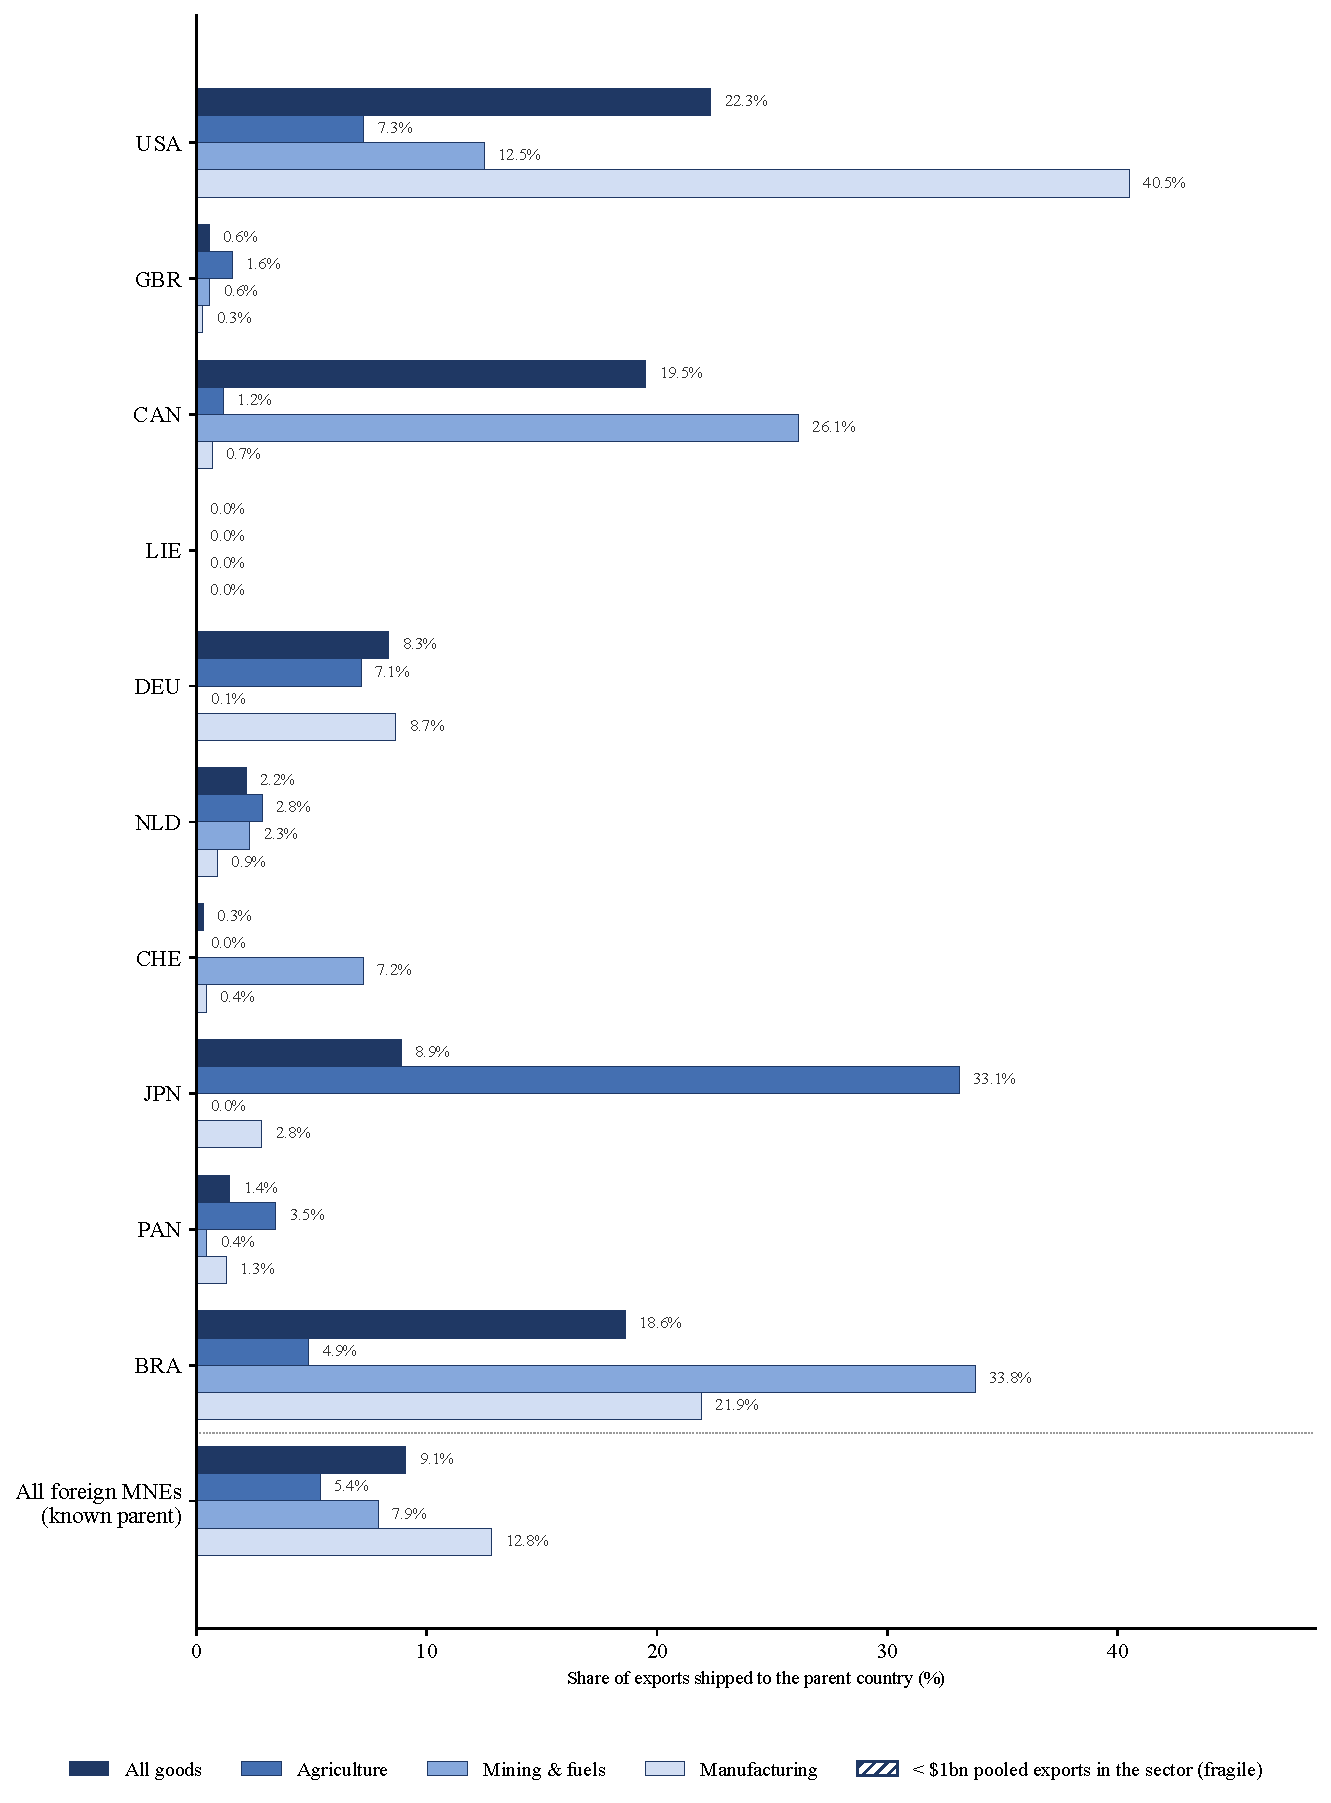
\includegraphics[width=0.95\textwidth,height=0.8\textheight,keepaspectratio]{figures/sectors/fig_wp3_home_share_by_parent_sectors.pdf}%
  \caption{Share of Foreign-Multinational Exports Shipped to the Parent Country, by Sector}%
  \label{fig:home_sectors}%
  \par\vspace{2pt}%
  \parbox{0.92\textwidth}{\footnotesize %
  \textit{Notes:} Percent of each parent country's exports shipped to that same country, by sector. Hatched bars: the parent country's exports in the sector are below US\$1 billion over the period.\\[3pt]%
  \textit{Source:} Authors' calculations based on customs data matched to Orbis and Dun \& Bradstreet.}%
  \end{figure}
% ---- Table: Share of Foreign-Multinational Exports Shipped to the Parent Country, by Sector
\begin{table}[H]\centering\footnotesize%
  \caption{Share of Foreign-Multinational Exports Shipped to the Parent Country, by Sector}%
  \label{tab:home_sectors_t}%
  \adjustbox{max width=\textwidth, max totalheight=0.8\textheight}{\begin{tabular}{lrrrrrrrr}
\toprule
 & \multicolumn{4}{c}{\% of the parent's exports shipped to the parent's country} & \multicolumn{4}{c}{Parent's exports (US\$bn/yr)} \\
Parent & All goods & Agriculture & Mining \& fuels & Manufacturing & All goods & Agriculture & Mining \& fuels & Manufacturing \\
\midrule
USA & 22.3 & 7.3 & 12.5 & 40.5 & 23.1 & 6.7 & 7.3 & 9.1 \\
GBR & 0.6 & 1.6 & 0.6 & 0.3 & 16.7 & 0.7 & 11.9 & 4.2 \\
CAN & 19.5 & 1.2 & 26.1 & 0.7 & 7.4 & 0.4 & 5.7 & 1.3 \\
LIE & 0.0 & 0.0 & 0.0 & 0.0 & 4.9 & 2.2 & 2.0 & 0.7 \\
DEU & 8.3 & 7.1 & 0.1 & 8.7 & 4.6 & 0.8 & 0.0 & 3.7 \\
NLD & 2.2 & 2.8 & 2.3 & 0.9 & 4.4 & 2.7 & 0.1 & 1.5 \\
CHE & 0.3 & 0.0 & 7.2 & 0.4 & 3.9 & 3.1 & 0.1 & 0.7 \\
JPN & 8.9 & 33.1 & 0.0 & 2.8 & 3.5 & 0.6 & 0.0 & 2.9 \\
PAN & 1.4 & 3.5 & 0.4 & 1.3 & 3.0 & 0.6 & 1.0 & 1.3 \\
BRA & 18.6 & 4.9 & 33.8 & 21.9 & 3.0 & 1.1 & 0.7 & 1.3 \\
\midrule
All known-parent foreign MNEs & 9.1 & 5.4 & 7.9 & 12.8 & 97.6 & 27.2 & 34.5 & 35.7 \\
\bottomrule
\end{tabular}
}%
  \par\vspace{3pt}%
  \begin{minipage}{0.95\textwidth}\footnotesize %
  \textit{Notes:} Left panel: percent of each parent country's exports shipped to that same country. Right panel: the parent country's exports. Values are annual averages in US\$ billion.\\[3pt]%
  \textit{Source:} Authors' calculations based on customs data matched to Orbis and Dun \& Bradstreet.%
  \end{minipage}%
  \end{table}

\subsection{Destination Markets}
% ---- Figure: Exports to the United States, by Type of Exporter and Exporting Country
\begin{figure}[H]\centering%
  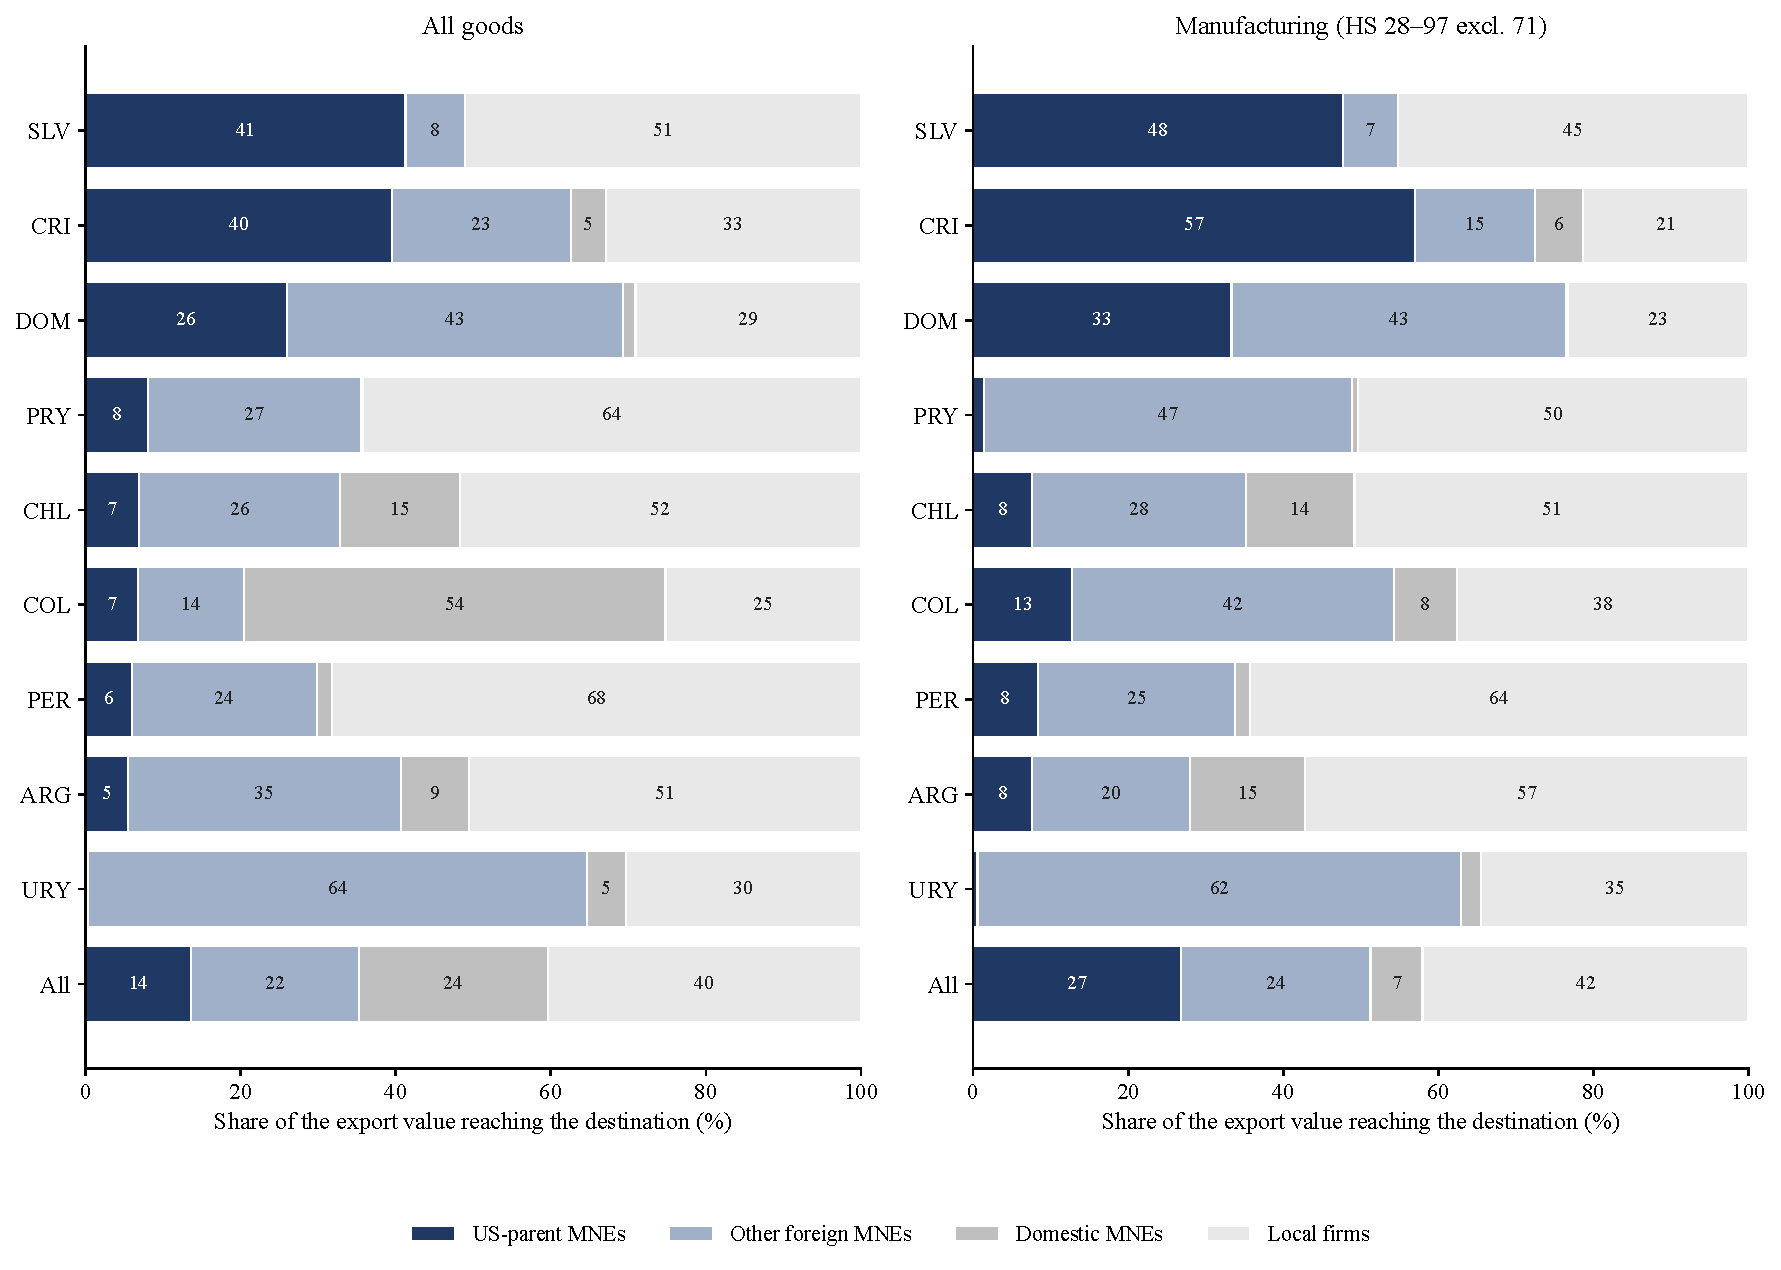
\includegraphics[width=1.0\textwidth,height=0.8\textheight,keepaspectratio]{figures/sectors/fig_wp3_to_usa_carriers_total_manuf.pdf}%
  \caption{Exports to the United States, by Type of Exporter and Exporting Country}%
  \label{fig:to_usa_tm}%
  \par\vspace{2pt}%
  \parbox{0.92\textwidth}{\footnotesize %
  \textit{Notes:} Percent of each country's exports to the United States, by type of exporter. Left: all goods. Right: manufacturing.\\[3pt]%
  \textit{Source:} Authors' calculations based on customs data matched to Orbis and Dun \& Bradstreet.}%
  \end{figure}
% ---- Table: Exports to the United States, by Type of Exporter and Sector
\begin{table}[H]\centering\small%
  \caption{Exports to the United States, by Type of Exporter and Sector}%
  \label{tab:to_usa_sec}%
  \adjustbox{max width=\textwidth, max totalheight=0.8\textheight}{\begin{tabular}{lrrrrr}
\toprule
Sector & Exports to the USA (US\$bn/yr) & US-parent MNEs (\%) & Other foreign MNEs (\%) & Domestic MNEs (\%) & Local firms (\%) \\
\midrule
\midrule
All goods & 40.0 & 13.6 & 21.6 & 24.4 & 40.4 \\
Agriculture & 10.7 & 4.8 & 28.0 & 9.2 & 58.0 \\
Mining \& fuels & 14.6 & 6.6 & 14.8 & 52.0 & 26.6 \\
Manufacturing & 14.5 & 26.8 & 24.4 & 6.7 & 42.1 \\
Rest & 0.1 & 40.0 & 38.4 & 4.5 & 17.1 \\
\bottomrule
\end{tabular}
}%
  \par\vspace{3pt}%
  \begin{minipage}{0.95\textwidth}\footnotesize %
  \textit{Notes:} Percent of each sector's exports to the United States, by type of exporter. Values are annual averages in US\$ billion.\\[3pt]%
  \textit{Source:} Authors' calculations based on customs data matched to Orbis and Dun \& Bradstreet.%
  \end{minipage}%
  \end{table}
% ---- Table: Exports to the United States, by Type of Exporter and Exporting Country
\begin{table}[H]\centering\small%
  \caption{Exports to the United States, by Type of Exporter and Exporting Country}%
  \label{tab:to_usa_all}%
  \adjustbox{max width=\textwidth, max totalheight=0.8\textheight}{\begin{tabular}{lrrrrr}
\toprule
Origin & Exports to the USA (US\$bn/yr) & US-parent MNEs (\%) & Other foreign MNEs (\%) & Domestic MNEs (\%) & Local firms (\%) \\
\midrule
SLV & 2.3 & 41.3 & 7.7 & 0.0 & 51.1 \\
CRI & 4.0 & 39.5 & 23.1 & 4.5 & 32.9 \\
DOM & 4.1 & 26.0 & 43.3 & 1.6 & 29.1 \\
PRY & 0.2 & 8.1 & 27.4 & 0.3 & 64.2 \\
CHL & 4.5 & 6.9 & 26.0 & 15.4 & 51.7 \\
COL & 13.8 & 6.8 & 13.7 & 54.4 & 25.2 \\
PER & 6.4 & 6.0 & 23.9 & 1.9 & 68.2 \\
ARG & 4.2 & 5.5 & 35.2 & 8.8 & 50.6 \\
URY & 0.4 & 0.4 & 64.3 & 5.0 & 30.3 \\
\midrule
All & 40.0 & 13.6 & 21.6 & 24.4 & 40.4 \\
\bottomrule
\end{tabular}
}%
  \par\vspace{3pt}%
  \begin{minipage}{0.95\textwidth}\footnotesize %
  \textit{Notes:} Percent of each country's exports to the United States, by type of exporter. Values are annual averages in US\$ billion.\\[3pt]%
  \textit{Source:} Authors' calculations based on customs data matched to Orbis and Dun \& Bradstreet.%
  \end{minipage}%
  \end{table}
% ---- Figure: Ownership of Exports to the Main Destination Markets
\begin{figure}[H]\centering%
  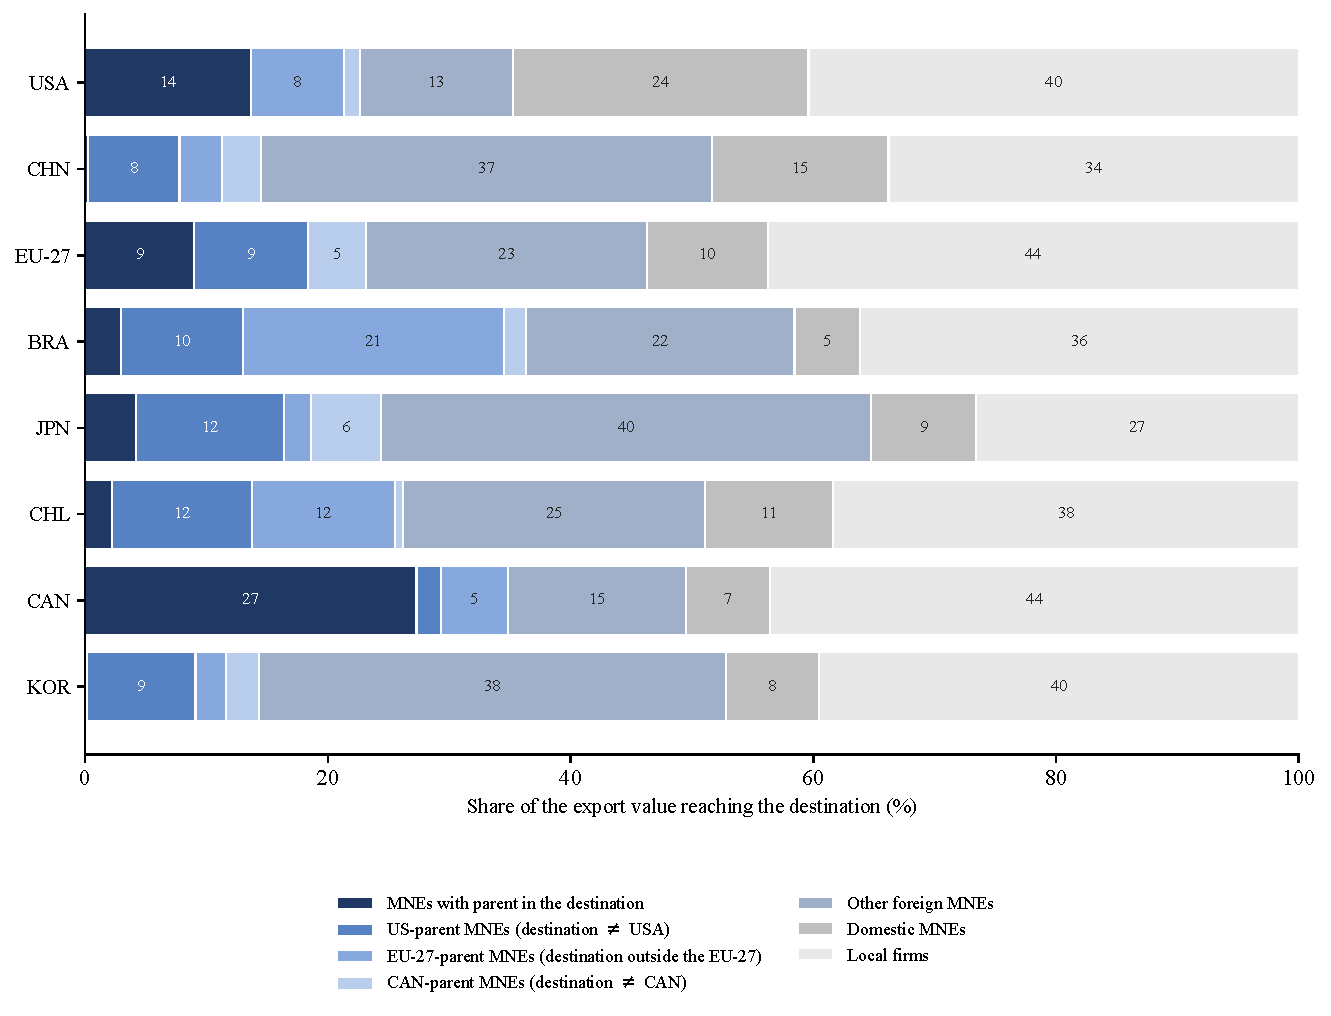
\includegraphics[width=0.95\textwidth,height=0.8\textheight,keepaspectratio]{figures/all/fig_wp3_dest_carriers.pdf}%
  \caption{Ownership of Exports to the Main Destination Markets}%
  \label{fig:dest_f_all}%
  \par\vspace{2pt}%
  \parbox{0.92\textwidth}{\footnotesize %
  \textit{Notes:} Percent of the export value reaching each destination, by type of exporter. The first segment is exports by MNEs whose parent is located in that destination. EU-27 member states are pooled.\\[3pt]%
  \textit{Source:} Authors' calculations based on customs data matched to Orbis and Dun \& Bradstreet.}%
  \end{figure}
% ---- Table: Ownership of Exports to the Main Destination Markets
\begin{table}[H]\centering\footnotesize%
  \caption{Ownership of Exports to the Main Destination Markets}%
  \label{tab:dest_all}%
  \adjustbox{max width=\textwidth, max totalheight=0.8\textheight}{\begin{tabular}{lrrrrrrrr}
\toprule
Destination & \multicolumn{1}{p{1.5cm}}{\raggedright Exports (US\$bn/yr)} & \multicolumn{1}{p{2.2cm}}{\raggedright MNEs with parent in the destination (\%)} & \multicolumn{1}{p{1.6cm}}{\raggedright US-parent MNEs (\%)} & \multicolumn{1}{p{1.6cm}}{\raggedright EU-27-parent MNEs (\%)} & \multicolumn{1}{p{1.6cm}}{\raggedright CAN-parent MNEs (\%)} & \multicolumn{1}{p{1.6cm}}{\raggedright Other foreign MNEs (\%)} & \multicolumn{1}{p{1.6cm}}{\raggedright Domestic MNEs (\%)} & \multicolumn{1}{p{1.5cm}}{\raggedright Local firms (\%)} \\
\midrule
USA & 40.0 & 13.6 & -- & 7.7 & 1.4 & 12.5 & 24.4 & 40.4 \\
CHN & 29.0 & 0.3 & 7.5 & 3.5 & 3.2 & 37.2 & 14.5 & 33.8 \\
EU-27 & 29.7 & 9.0 & 9.4 & -- & 4.8 & 23.1 & 9.9 & 43.8 \\
BRA & 20.0 & 2.9 & 10.1 & 21.5 & 1.8 & 22.1 & 5.4 & 36.1 \\
JPN & 6.5 & 4.2 & 12.2 & 2.2 & 5.8 & 40.4 & 8.6 & 26.6 \\
CHL & 6.6 & 2.2 & 11.5 & 11.8 & 0.7 & 24.9 & 10.6 & 38.4 \\
CAN & 6.0 & 27.3 & 2.0 & 5.5 & -- & 14.7 & 6.9 & 43.5 \\
KOR & 5.0 & 0.1 & 9.0 & 2.5 & 2.7 & 38.5 & 7.7 & 39.5 \\
\bottomrule
\end{tabular}
}%
  \par\vspace{3pt}%
  \begin{minipage}{0.95\textwidth}\footnotesize %
  \textit{Notes:} Percent of the export value reaching each destination, by type of exporter. EU-27 member states are pooled. Values are annual averages in US\$ billion.\\[3pt]%
  \textit{Source:} Authors' calculations based on customs data matched to Orbis and Dun \& Bradstreet.%
  \end{minipage}%
  \end{table}
% ---- Table: Main Products Shipped by US-Parent Multinationals to the United States
\begin{table}[H]\centering\footnotesize%
  \caption{Main Products Shipped by US-Parent Multinationals to the United States}%
  \label{tab:us_home_all}%
  \adjustbox{max width=\textwidth, max totalheight=0.8\textheight}{\begin{tabular}{llrrrrrl}
\toprule
HS6 & Description & \multicolumn{1}{p{1.7cm}}{\raggedright US-parent exports to the USA (US\$bn/yr)} & \multicolumn{1}{p{1.7cm}}{\raggedright \% of all US-parent exports to the USA} & \multicolumn{1}{p{2.0cm}}{\raggedright \% of US-parent exports of the product going to the USA} & \multicolumn{1}{p{1.9cm}}{\raggedright All exports of the product to the USA (US\$bn/yr)} & \multicolumn{1}{p{2.2cm}}{\raggedright US-parent share of exports of the product to the USA (\%)} & \multicolumn{1}{p{2.6cm}}{\raggedright Main origins of the US-parent shipments (\% of the line)} \\
\midrule
610910 & T-shirts, singlets \& other vests, knitted/cro... & 0.49 & 11.1 & 84 & 1.01 & 53 & SLV 85\%, DOM 10\%, PER 5\% \\
901839 & Catheters, cannulae \& the like & 0.52 & 9.6 & 73 & 0.63 & 89 & CRI 92\%, DOM 8\%, COL 0\% \\
270900 & Petroleum oils \& oils obt. from bituminous mi... & 0.41 & 9.1 & 24 & 7.84 & 5 & COL 100\%, ARG 0\% \\
901890 & Instruments \& appliances used in medical/surg... & 0.39 & 6.8 & 69 & 0.94 & 47 & CRI 71\%, DOM 29\%, COL 0\% \\
270112 & Bituminous coal, whether/not pulverised but n... & 0.19 & 4.3 & 9 & 0.39 & 48 & COL 100\% \\
854231 & Electronic integrated circuits, processors \& ... & 0.21 & 3.9 & 28 & 0.22 & 95 & CRI 100\%, COL 0\%, ARG 0\% \\
401110 & New pneumatic tyres, of rubber, of a kind use... & 0.13 & 3.4 & 93 & 0.24 & 63 & CHL 100\%, DOM 0\%, COL 0\% \\
261390 & Molybdenum ores \& concentrates, other than ro... & 0.15 & 2.8 & 99 & 0.18 & 79 & PER 100\% \\
611595 & Other n.e.s. in 61.15, knitted/crocheted, of ... & 0.10 & 2.4 & 100 & 0.11 & 97 & SLV 100\%, DOM 0\% \\
610711 & Men's/boys' underpants \& briefs, knitted/croc... & 0.09 & 2.2 & 87 & 0.10 & 87 & SLV 100\%, DOM 0\%, CRI 0\% \\
621210 & Brassieres \& parts thereof , whether/not knit... & 0.09 & 1.8 & 98 & 0.12 & 78 & SLV 74\%, DOM 26\%, CRI 0\% \\
080430 & Pineapples, fresh/dried & 0.08 & 1.6 & 66 & 0.42 & 20 & CRI 100\% \\
240210 & Cigars, cheroots \& cigarillos containing toba... & 0.09 & 1.3 & 100 & 0.57 & 16 & DOM 100\% \\
740311 & Cathodes \& sections of cathodes, of refined c... & 0.06 & 1.2 & 24 & 1.56 & 3 & PER 64\%, CHL 36\% \\
640510 & Footwear with uppers of leather/composition l... & 0.08 & 1.2 & 70 & 0.11 & 71 & DOM 100\% \\
\midrule
All lines & & 5.0 & 100.0 & 22 & 40.0 & 14 & \\
\bottomrule
\end{tabular}
}%
  \par\vspace{3pt}%
  \begin{minipage}{0.95\textwidth}\footnotesize %
  \textit{Notes:} Fifteen HS6 products with the largest exports by US-parent MNEs to the United States. Values are annual averages in US\$ billion.\\[3pt]%
  \textit{Source:} Authors' calculations based on customs data matched to Orbis and Dun \& Bradstreet.%
  \end{minipage}%
  \end{table}
% ---- Figure: US-Parent Share of Exports to the United States, Main Products Shipped by US-Parent Multinationals
\begin{figure}[H]\centering%
  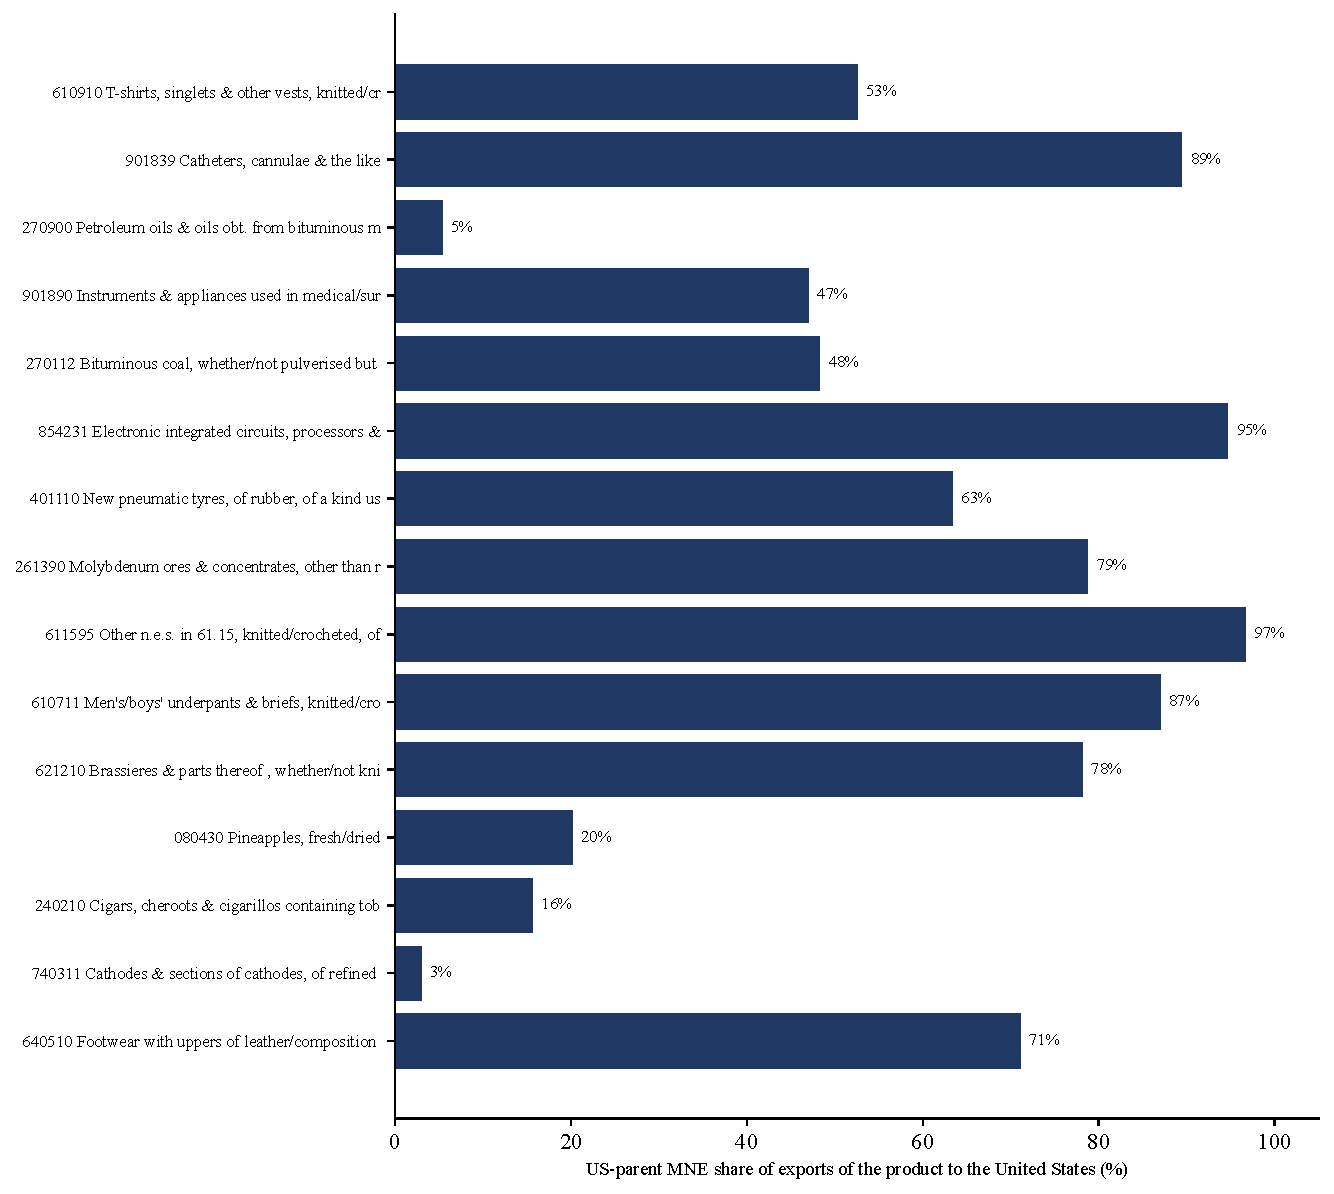
\includegraphics[width=0.95\textwidth,height=0.8\textheight,keepaspectratio]{figures/all/fig_wp3_us_home_products.pdf}%
  \caption{US-Parent Share of Exports to the United States, Main Products Shipped by US-Parent Multinationals}%
  \label{fig:us_home_f_all}%
  \par\vspace{2pt}%
  \parbox{0.92\textwidth}{\footnotesize %
  \textit{Notes:} Percent of the nine countries' exports of each product to the United States shipped by US-parent MNEs; the fifteen products with the largest US-parent exports to the United States.\\[3pt]%
  \textit{Source:} Authors' calculations based on customs data matched to Orbis and Dun \& Bradstreet.}%
  \end{figure}
% ---- Table: Largest Export Products to the United States, by Type of Exporter
\begin{table}[H]\centering\footnotesize%
  \caption{Largest Export Products to the United States, by Type of Exporter}%
  \label{tab:to_usa_prod_all}%
  \adjustbox{max width=\textwidth, max totalheight=0.8\textheight}{\begin{tabular}{llrrrrr}
\toprule
HS6 & Description & \multicolumn{1}{p{2.0cm}}{\raggedright Exports to the USA (US\$bn/yr)} & \multicolumn{1}{p{1.8cm}}{\raggedright US-parent MNEs (\%)} & \multicolumn{1}{p{1.8cm}}{\raggedright Other foreign MNEs (\%)} & \multicolumn{1}{p{1.8cm}}{\raggedright Domestic MNEs (\%)} & \multicolumn{1}{p{1.8cm}}{\raggedright Local firms (\%)} \\
\midrule
270900 & Petroleum oils \& oils obt. from bituminous mi... & 7.84 & 5 & 10 & 81 & 4 \\
710812 & Gold (incl. gold plated with platinum), in un... & 2.72 & 1 & 16 & 9 & 74 \\
740311 & Cathodes \& sections of cathodes, of refined c... & 1.56 & 3 & 33 & 4 & 60 \\
090111 & Coffee, not roasted, not decaffeinated & 1.42 & 3 & 36 & 8 & 53 \\
271019 & Petroleum oils \& oils obtained from bituminou... & 1.14 & 0 & 14 & 51 & 35 \\
610910 & T-shirts, singlets \& other vests, knitted/cro... & 1.01 & 53 & 7 & 0 & 40 \\
901890 & Instruments \& appliances used in medical/surg... & 0.94 & 47 & 44 & 0 & 9 \\
060319 & Cut flowers \& flower buds of a kind suit. for... & 0.61 & 1 & 19 & 19 & 60 \\
271011 & Light petroleum oils \& preparations & 0.69 & 4 & 14 & 5 & 76 \\
901839 & Catheters, cannulae \& the like & 0.63 & 89 & 2 & 0 & 9 \\
030441 & Fish fillets\&other fish meat (excl. of 0304.1... & 0.38 & 2 & 18 & 24 & 56 \\
080610 & Grapes, fresh & 0.39 & 5 & 27 & 10 & 58 \\
270112 & Bituminous coal, whether/not pulverised but n... & 0.39 & 48 & 32 & 1 & 19 \\
240210 & Cigars, cheroots \& cigarillos containing toba... & 0.57 & 16 & 47 & 0 & 37 \\
080390 & Bananas, fresh or dried (excl. plantains) [HS... & 0.43 & 14 & 27 & 1 & 58 \\
\bottomrule
\end{tabular}
}%
  \par\vspace{3pt}%
  \begin{minipage}{0.95\textwidth}\footnotesize %
  \textit{Notes:} Fifteen largest HS6 products exported to the United States; percent of each product's exports to the United States by type of exporter. Values are annual averages in US\$ billion.\\[3pt]%
  \textit{Source:} Authors' calculations based on customs data matched to Orbis and Dun \& Bradstreet.%
  \end{minipage}%
  \end{table}

\section{Fact 4: A Small Set of Large Multinational Groups Accounts for Most Exports}\label{sec:f4s_all}

\subsection{Size of the Group's Global Network}
% ---- Figure: Foreign-Multinational Exports and Number of Parents, by Size of the Group's Global Network
\begin{figure}[H]\centering%
  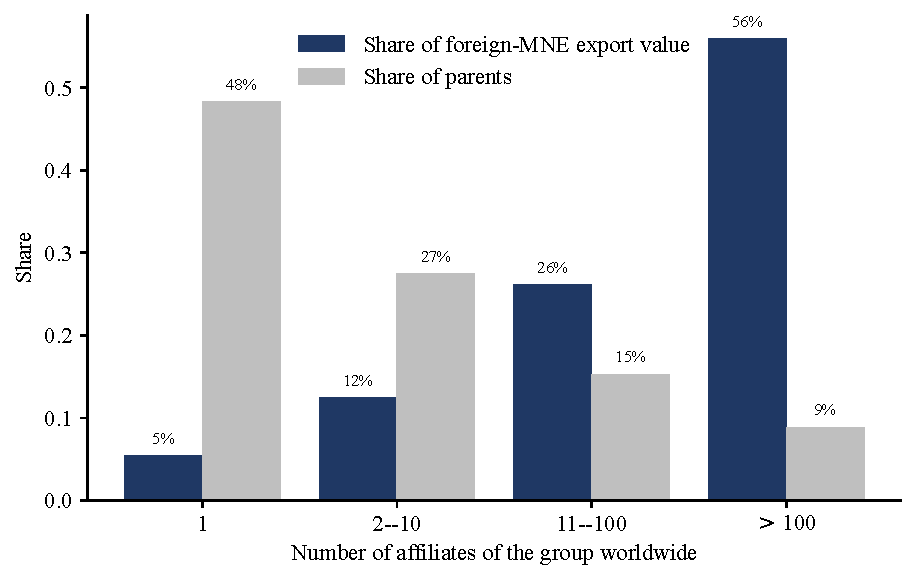
\includegraphics[width=0.7\textwidth,height=0.8\textheight,keepaspectratio]{figures/all/fig_wp0_fig5_network.pdf}%
  \caption{Foreign-Multinational Exports and Number of Parents, by Size of the Group's Global Network}%
  \label{fig:net_all}%
  \par\vspace{2pt}%
  \parbox{0.92\textwidth}{\footnotesize %
  \textit{Notes:} Shares of foreign-MNE export value and of parents, by the number of affiliates the group has worldwide.\\[3pt]%
  \textit{Source:} Authors' calculations based on customs data matched to Orbis and Dun \& Bradstreet.}%
  \end{figure}
% ---- Table: Foreign-Multinational Exports and Number of Parents, by Size of the Group's Global Network
\begin{table}[H]\centering\small%
  \caption{Foreign-Multinational Exports and Number of Parents, by Size of the Group's Global Network}%
  \label{tab:net_t_all}%
  \adjustbox{max width=\textwidth, max totalheight=0.8\textheight}{\begin{tabular}{lrrr}
\toprule
Affiliates worldwide & Parents & Share of parents (\%) & Share of foreign-MNE export value (\%) \\
\midrule
1 & 5,982 & 48.4 & 5.4 \\
2--10 & 3,397 & 27.5 & 12.4 \\
11--100 & 1,893 & 15.3 & 26.2 \\
$>$100 & 1,099 & 8.9 & 56.0 \\
\midrule
All parents & 12,371 & 100 & 100 \\
\bottomrule
\end{tabular}
}%
  \par\vspace{3pt}%
  \begin{minipage}{0.95\textwidth}\footnotesize %
  \textit{Notes:} Number and share of parents, and share of foreign-MNE export value, by the number of affiliates the group has worldwide.\\[3pt]%
  \textit{Source:} Authors' calculations based on customs data matched to Orbis and Dun \& Bradstreet.%
  \end{minipage}%
  \end{table}

\subsection{Concentration within Products}
% ---- Figure: Export Concentration within Products: Firms and Groups
\begin{figure}[H]\centering%
  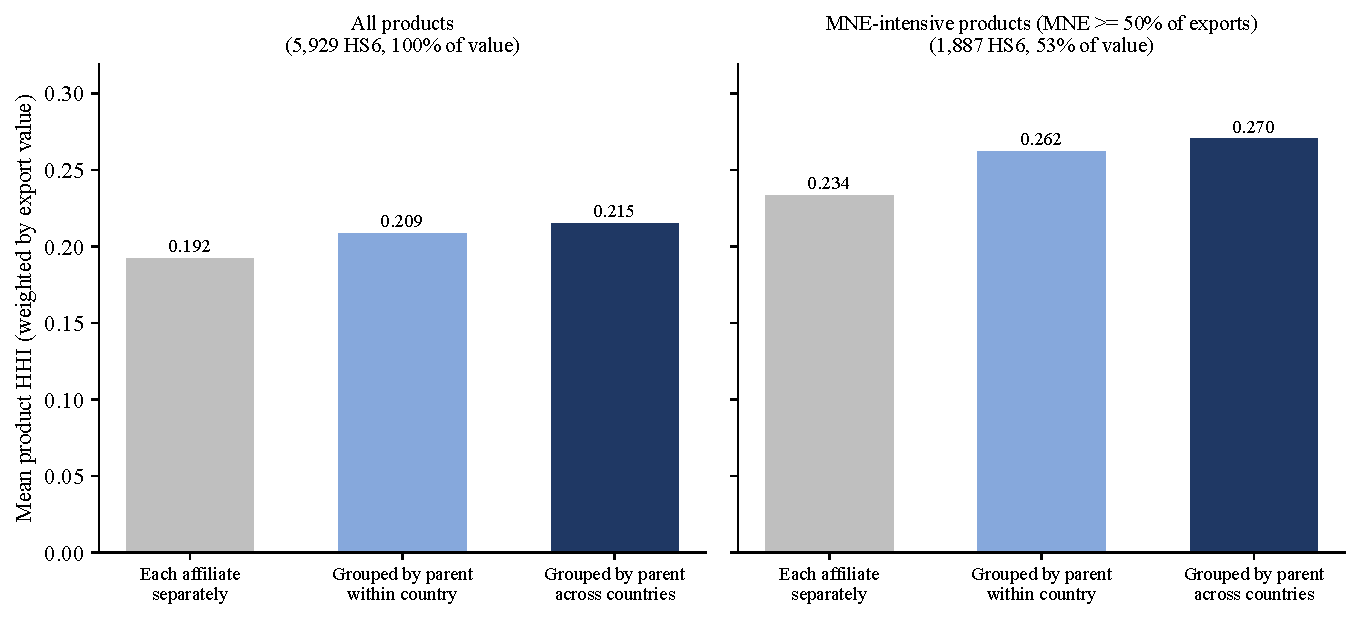
\includegraphics[width=0.9\textwidth,height=0.8\textheight,keepaspectratio]{figures/all/fig_wp0_fig6_hhi.pdf}%
  \caption{Export Concentration within Products: Firms and Groups}%
  \label{fig:hhi_all}%
  \par\vspace{2pt}%
  \parbox{0.92\textwidth}{\footnotesize %
  \textit{Notes:} Mean Herfindahl index of exporters within each HS6 product, weighted by export value, counting each affiliate separately or grouping affiliates by parent within or across countries. Right panel: products where MNEs account for at least half of exports.\\[3pt]%
  \textit{Source:} Authors' calculations based on customs data matched to Orbis and Dun \& Bradstreet.}%
  \end{figure}
% ---- Table: Export Concentration within Products: Firms and Groups
\begin{table}[H]\centering\small%
  \caption{Export Concentration within Products: Firms and Groups}%
  \label{tab:hhi_t_all}%
  \adjustbox{max width=\textwidth, max totalheight=0.8\textheight}{\begin{tabular}{llrrr}
\toprule
Sample & Measure & Firm level & Groups within country & Groups across countries \\
\midrule
\multicolumn{5}{l}{\textit{All products: 5,929 HS6, 100\% of value}} \\
 & Mean HHI & 0.192 & 0.209 & 0.215 \\
 & Mean top-exporter share & 31.0\% & 32.5\% & 33.7\% \\
 & Effective number of exporters (1/HHI) & 12.5 & 11.7 & 10.4 \\
\multicolumn{5}{l}{\textit{MNE-intensive products (MNE $\geq$ 50\% of exports): 1,887 HS6, 53\% of value}} \\
 & Mean HHI & 0.234 & 0.262 & 0.270 \\
 & Mean top-exporter share & 36.0\% & 38.7\% & 39.8\% \\
 & Effective number of exporters (1/HHI) & 8.9 & 8.0 & 7.4 \\
\bottomrule
\end{tabular}
}%
  \par\vspace{3pt}%
  \begin{minipage}{0.95\textwidth}\footnotesize %
  \textit{Notes:} Means across HS6 products, weighted by export value. Firm level: each affiliate counted separately. Groups: affiliates grouped by ultimate parent within each exporting country or across countries.\\[3pt]%
  \textit{Source:} Authors' calculations based on customs data matched to Orbis and Dun \& Bradstreet.%
  \end{minipage}%
  \end{table}

\subsection{Groups and Affiliates}
% ---- Table: Multinational Affiliates and Groups in Origin--Destination--Product--Year Cells
\begin{table}[H]\centering\small%
  \caption{Multinational Affiliates and Groups in Origin--Destination--Product--Year Cells}%
  \label{tab:grp_all}%
  \adjustbox{max width=\textwidth, max totalheight=0.8\textheight}{\begin{tabular}{lr}
\toprule
Origin-destination-product-year cells with $\geq 1$ MNE & \\
\midrule
Cells & 1,008,755 \\
MNE affiliates per cell (mean) & 1.91 \\
MNE groups per cell (mean) & 1.90 \\
Affiliates per group, pooled & 1.01 \\
Affiliates per group, mean weighted by export value & 1.08 \\
Cells where one group exports through $>1$ affiliate (\%) & 1.0 \\
\bottomrule
\end{tabular}
}%
  \par\vspace{3pt}%
  \begin{minipage}{0.95\textwidth}\footnotesize %
  \textit{Notes:} Cells with at least one MNE. Group: ultimate parent in Orbis or Dun \& Bradstreet (parent name when the identifier is missing).\\[3pt]%
  \textit{Source:} Authors' calculations based on customs data matched to Orbis and Dun \& Bradstreet.%
  \end{minipage}%
  \end{table}
% ---- Table: Multinational Presence and Exports: Affiliates and Groups
\begin{table}[H]\centering\small%
  \caption{Multinational Presence and Exports: Affiliates and Groups}%
  \label{tab:grp_r_all}%
  \adjustbox{max width=\textwidth, max totalheight=0.8\textheight}{\begin{tabular}{lcccccc} \hline
 & \multicolumn{3}{c}{Origin $\times$ year, destination $\times$ year, product FE} & \multicolumn{3}{c}{Origin $\times$ dest. $\times$ product, origin $\times$ dest. $\times$ year FE} \\
 & (1) & (2) & (3) & (4) & (5) & (6) \\ \hline
\multicolumn{7}{l}{\textit{Panel A. Dependent variable: $\ln$ exports, all firms}} \\
$\ln$(\# MNE firms) & 2.0685*** &  &  & 0.9414*** &  &  \\
 & (0.0368) &  &  & (0.0206) &  &  \\
$\ln$(\# MNE groups) &  & 2.0728*** & 2.0617*** &  & 0.9416*** & 0.9421*** \\
 &  & (0.0371) & (0.0365) &  & (0.0208) & (0.0208) \\
$\ln$(affiliates per group) &  &  & 2.7723*** &  &  & 0.8692*** \\
 &  &  & (0.2413) &  &  & (0.0648) \\
\midrule
\multicolumn{7}{l}{\textit{Panel B. Dependent variable: $\ln$ exports, non-MNE firms}} \\
$\ln$(\# MNE firms) & 1.3406*** &  &  & 0.2389*** &  &  \\
 & (0.0319) &  &  & (0.0178) &  &  \\
$\ln$(\# MNE groups) &  & 1.3471*** & 1.3427*** &  & 0.2400*** & 0.2400*** \\
 &  & (0.0319) & (0.0317) &  & (0.0177) & (0.0177) \\
$\ln$(affiliates per group) &  &  & 1.1055*** &  &  & 0.0605 \\
 &  &  & (0.2963) &  &  & (0.0985) \\
\hline
Product FE & $\checkmark$ & $\checkmark$ & $\checkmark$ &  &  &  \\
Origin $\times$ year FE & $\checkmark$ & $\checkmark$ & $\checkmark$ &  &  &  \\
Destination $\times$ year FE & $\checkmark$ & $\checkmark$ & $\checkmark$ &  &  &  \\
Origin $\times$ dest.\ $\times$ product FE &  &  &  & $\checkmark$ & $\checkmark$ & $\checkmark$ \\
Origin $\times$ dest.\ $\times$ year FE &  &  &  & $\checkmark$ & $\checkmark$ & $\checkmark$ \\
Observations (Panel A) & 1,008,185 & 1,008,185 & 1,008,185 & 883,545 & 883,545 & 883,545 \\
Observations (Panel B) & 475,514 & 475,514 & 475,514 & 429,882 & 429,882 & 429,882 \\
\hline
\end{tabular}
}%
  \par\vspace{3pt}%
  \begin{minipage}{0.95\textwidth}\footnotesize %
  \textit{Notes:} Observations are origin--destination--HS6--year cells. Dependent variable: $\ln$ exports of the cell (Panel A) and of the non-MNE firms in the cell (Panel B). Regressors: $\ln$ number of MNE affiliates or $\ln$ number of MNE groups (distinct ultimate parents). Standard errors clustered by origin--destination pair in parentheses. *** $p<0.01$, ** $p<0.05$, * $p<0.1$.\\[3pt]%
  \textit{Source:} Authors' calculations based on customs data matched to Orbis and Dun \& Bradstreet.%
  \end{minipage}%
  \end{table}

\section{Fact 5: Multinational Presence Is Associated with Higher Exports}\label{sec:f5_all}
% ---- Table: Multinational Presence and Exports
\begin{table}[H]\centering\small%
  \caption{Multinational Presence and Exports}%
  \label{tab:t1_all}%
  \adjustbox{max width=\textwidth, max totalheight=0.8\textheight}{\begin{tabular}{lcccccc} \hline
 & \multicolumn{3}{c}{Intensive: $\ln$(\# MNE firms)} & \multicolumn{3}{c}{Extensive: any MNE present} \\
 & (1) & (2) & (3) & (1) & (2) & (3) \\ \hline
\multicolumn{7}{l}{\textit{Panel A. Dependent variable: $\ln$ exports, all firms}} \\
$\ln$(\# MNE firms) & 2.0823*** & 2.0685*** & 0.9414*** &  &  &  \\
 & (0.0363) & (0.0368) & (0.0206) &  &  &  \\
Any MNE present &  &  &  & 1.4622*** & 1.4591*** & 0.6818*** \\
 &  &  &  & (0.0394) & (0.0388) & (0.0165) \\
\midrule
\multicolumn{7}{l}{\textit{Panel B. Dependent variable: $\ln$ exports, non-MNE firms}} \\
$\ln$(\# MNE firms) & 1.3536*** & 1.3406*** & 0.2389*** &  &  &  \\
 & (0.0318) & (0.0319) & (0.0178) &  &  &  \\
Any MNE present &  &  &  & 1.4168*** & 1.3996*** & 0.1311*** \\
 &  &  &  & (0.0371) & (0.0367) & (0.0102) \\
\hline
Origin FE & $\checkmark$ &  &  & $\checkmark$ &  &  \\
Destination FE & $\checkmark$ &  &  & $\checkmark$ &  &  \\
Product FE & $\checkmark$ & $\checkmark$ &  & $\checkmark$ & $\checkmark$ &  \\
Year FE & $\checkmark$ &  &  & $\checkmark$ &  &  \\
Origin $\times$ year FE &  & $\checkmark$ &  &  & $\checkmark$ &  \\
Destination $\times$ year FE &  & $\checkmark$ &  &  & $\checkmark$ &  \\
Origin $\times$ dest.\ $\times$ product FE &  &  & $\checkmark$ &  &  & $\checkmark$ \\
Origin $\times$ dest.\ $\times$ year FE &  &  & $\checkmark$ &  &  & $\checkmark$ \\
Observations (Panel A) & 1,008,472 & 1,008,185 & 883,545 & 1,829,852 & 1,829,626 & 1,633,319 \\
Observations (Panel B) & 475,856 & 475,514 & 429,882 & 1,297,322 & 1,297,111 & 1,137,550 \\
\hline
\end{tabular}
}%
  \par\vspace{3pt}%
  \begin{minipage}{0.95\textwidth}\footnotesize %
  \textit{Notes:} Observations are origin--destination--HS6--year cells. Dependent variable: $\ln$ exports of the cell (Panel A) and of the non-MNE firms in the cell (Panel B). Intensive margin: $\ln$ number of MNEs, cells with at least one MNE. Extensive margin: indicator for at least one MNE. Standard errors clustered by origin--destination pair in parentheses. *** $p<0.01$, ** $p<0.05$, * $p<0.1$.\\[3pt]%
  \textit{Source:} Authors' calculations based on customs data matched to Orbis and Dun \& Bradstreet.%
  \end{minipage}%
  \end{table}
% ---- Table: Multinational Exports by Exporting Country and Destination Type
\begin{table}[H]\centering\small%
  \caption{Multinational Exports by Exporting Country and Destination Type}%
  \label{tab:pres_all}%
  \adjustbox{max width=\textwidth, max totalheight=0.8\textheight}{\begin{tabular}{lrrrrr}
\toprule
Origin & MNE value (US\$bn/yr) & of which domestic (\%) & Foreign-MNE value (US\$bn/yr) & \multicolumn{2}{c}{\% of foreign-MNE value, by destination} \\
 & & & & parent country & other (of which: group affiliate there) \\
\midrule
ARG & 37.5 & 13.3 & 32.5 & 6.5 & 93.5 (41.8) \\
CHL & 21.0 & 22.1 & 16.4 & 4.3 & 95.7 (56.7) \\
COL & 32.8 & 52.5 & 15.5 & 6.5 & 93.5 (34.2) \\
CRI & 6.6 & 5.7 & 6.3 & 25.5 & 74.5 (33.8) \\
DOM & 6.0 & 1.8 & 5.9 & 29.0 & 71.0 (21.6) \\
PER & 19.3 & 5.0 & 18.3 & 3.9 & 96.1 (28.8) \\
PRY & 4.5 & 1.8 & 4.4 & 2.1 & 97.9 (65.5) \\
SLV & 2.4 & 0.6 & 2.4 & 40.7 & 59.3 (28.1) \\
URY & 4.4 & 15.9 & 3.7 & 5.2 & 94.8 (37.7) \\
\midrule
All & 134.5 & 23.4 & 105.4 & 8.4 & 91.6 (40.5) \\
\bottomrule
\end{tabular}
}%
  \par\vspace{3pt}%
  \begin{minipage}{0.95\textwidth}\footnotesize %
  \textit{Notes:} MNE and foreign-MNE export value by country, and the split of foreign-MNE value by destination. Parent country: exports to the country of the ultimate parent. Other: all remaining destinations; in parentheses, destinations where the group has another affiliate. Values are annual averages in US\$ billion.\\[3pt]%
  \textit{Source:} Authors' calculations based on customs data matched to Orbis and Dun \& Bradstreet.%
  \end{minipage}%
  \end{table}
% ---- Table: Multinational Presence and Exports: Intensive Margin, by Type of Multinational
\begin{table}[H]\centering\small%
  \caption{Multinational Presence and Exports: Intensive Margin, by Type of Multinational}%
  \label{tab:cnt_all}%
  \adjustbox{max width=\textwidth, max totalheight=0.8\textheight}{\begin{tabular}{lcccccc} \hline
 & \multicolumn{2}{c}{All MNEs} & \multicolumn{2}{c}{Foreign / domestic} & \multicolumn{2}{c}{Foreign by destination, domestic} \\
 & (1) & (2) & (3) & (4) & (5) & (6) \\ \hline
\multicolumn{7}{l}{\textit{Panel A. Dependent variable: $\ln$ exports, all firms}} \\
$\ln$(\# MNE firms) & 2.0685*** & 0.9414*** &  &  &  &  \\
 & (0.0368) & (0.0206) &  &  &  &  \\
$\ln$(\# foreign MNEs) &  &  & 1.2129*** & 0.4506*** &  &  \\
 &  &  & (0.0285) & (0.0124) &  &  \\
$\ln$(\# foreign MNEs, parent-country destination) &  &  &  &  & 0.3970*** & 0.1448*** \\
 &  &  &  &  & (0.0856) & (0.0370) \\
$\ln$(\# foreign MNEs, other destinations) &  &  &  &  & 0.9465*** & 0.3133*** \\
 &  &  &  &  & (0.0536) & (0.0382) \\
$\ln$(\# domestic MNEs) &  &  & 0.4382*** & 0.2214*** & 0.3770*** & 0.1555*** \\
 &  &  & (0.0259) & (0.0151) & (0.0514) & (0.0315) \\
\midrule
\multicolumn{7}{l}{\textit{Panel B. Dependent variable: $\ln$ exports, non-MNE firms}} \\
$\ln$(\# MNE firms) & 1.3406*** & 0.2389*** &  &  &  &  \\
 & (0.0319) & (0.0178) &  &  &  &  \\
$\ln$(\# foreign MNEs) &  &  & 1.1331*** & 0.2413*** &  &  \\
 &  &  & (0.0375) & (0.0217) &  &  \\
$\ln$(\# foreign MNEs, parent-country destination) &  &  &  &  & 0.2934*** & 0.1945*** \\
 &  &  &  &  & (0.0882) & (0.0527) \\
$\ln$(\# foreign MNEs, other destinations) &  &  &  &  & 1.0330*** & 0.1951*** \\
 &  &  &  &  & (0.0607) & (0.0648) \\
$\ln$(\# domestic MNEs) &  &  & 0.4707*** & 0.1250*** & 0.4142*** & 0.0946* \\
 &  &  & (0.0341) & (0.0218) & (0.0633) & (0.0552) \\
\hline
Product FE & $\checkmark$ &  & $\checkmark$ &  & $\checkmark$ &  \\
Origin $\times$ year FE & $\checkmark$ &  & $\checkmark$ &  & $\checkmark$ &  \\
Destination $\times$ year FE & $\checkmark$ &  & $\checkmark$ &  & $\checkmark$ &  \\
Origin $\times$ dest.\ $\times$ product FE &  & $\checkmark$ &  & $\checkmark$ &  & $\checkmark$ \\
Origin $\times$ dest.\ $\times$ year FE &  & $\checkmark$ &  & $\checkmark$ &  & $\checkmark$ \\
Observations (Panel A) & 1,008,185 & 883,545 & 113,422 & 98,223 & 9,197 & 7,524 \\
Observations (Panel B) & 475,514 & 429,882 & 93,010 & 81,563 & 8,780 & 7,255 \\
\hline
\end{tabular}
}%
  \par\vspace{3pt}%
  \begin{minipage}{0.95\textwidth}\footnotesize %
  \textit{Notes:} Observations are origin--destination--HS6--year cells. Dependent variable: $\ln$ exports of the cell (Panel A) and of the non-MNE firms in the cell (Panel B). Regressors: $\ln$ number of MNEs of each type. Columns (5)--(6) split foreign MNEs by whether the destination is the parent's country. Standard errors clustered by origin--destination pair in parentheses. *** $p<0.01$, ** $p<0.05$, * $p<0.1$.\\[3pt]%
  \textit{Source:} Authors' calculations based on customs data matched to Orbis and Dun \& Bradstreet.%
  \end{minipage}%
  \end{table}
% ---- Table: Multinational Presence and Exports: Extensive Margin, by Type of Multinational
\begin{table}[H]\centering\small%
  \caption{Multinational Presence and Exports: Extensive Margin, by Type of Multinational}%
  \label{tab:ext_all}%
  \adjustbox{max width=\textwidth, max totalheight=0.8\textheight}{\begin{tabular}{lcccccc} \hline
 & \multicolumn{2}{c}{All MNEs} & \multicolumn{2}{c}{Foreign / domestic} & \multicolumn{2}{c}{Foreign by destination, domestic} \\
 & (1) & (2) & (3) & (4) & (5) & (6) \\ \hline
\multicolumn{7}{l}{\textit{Panel A. Dependent variable: $\ln$ exports, all firms}} \\
Any MNE present & 1.4591*** & 0.6818*** &  &  &  &  \\
 & (0.0388) & (0.0165) &  &  &  &  \\
Any foreign MNE &  &  & 1.4990*** & 0.6986*** &  &  \\
 &  &  & (0.0339) & (0.0158) &  &  \\
Any foreign MNE, parent-country destination &  &  &  &  & 1.3873*** & 0.5909*** \\
 &  &  &  &  & (0.0951) & (0.0431) \\
Any foreign MNE, other destination &  &  &  &  & 1.5093*** & 0.6976*** \\
 &  &  &  &  & (0.0319) & (0.0146) \\
Any domestic MNE &  &  & 1.4670*** & 0.4917*** & 1.4334*** & 0.4909*** \\
 &  &  & (0.0416) & (0.0165) & (0.0388) & (0.0166) \\
\midrule
\multicolumn{7}{l}{\textit{Panel B. Dependent variable: $\ln$ exports, non-MNE firms}} \\
Any MNE present & 1.3996*** & 0.1311*** &  &  &  &  \\
 & (0.0367) & (0.0102) &  &  &  &  \\
Any foreign MNE &  &  & 1.2983*** & 0.1356*** &  &  \\
 &  &  & (0.0346) & (0.0106) &  &  \\
Any foreign MNE, parent-country destination &  &  &  &  & 1.0183*** & 0.1265*** \\
 &  &  &  &  & (0.0900) & (0.0194) \\
Any foreign MNE, other destination &  &  &  &  & 1.2782*** & 0.1386*** \\
 &  &  &  &  & (0.0326) & (0.0107) \\
Any domestic MNE &  &  & 1.1316*** & 0.1370*** & 1.0959*** & 0.1367*** \\
 &  &  & (0.0428) & (0.0138) & (0.0403) & (0.0138) \\
\hline
Product FE & $\checkmark$ &  & $\checkmark$ &  & $\checkmark$ &  \\
Origin $\times$ year FE & $\checkmark$ &  & $\checkmark$ &  & $\checkmark$ &  \\
Destination $\times$ year FE & $\checkmark$ &  & $\checkmark$ &  & $\checkmark$ &  \\
Origin $\times$ dest.\ $\times$ product FE &  & $\checkmark$ &  & $\checkmark$ &  & $\checkmark$ \\
Origin $\times$ dest.\ $\times$ year FE &  & $\checkmark$ &  & $\checkmark$ &  & $\checkmark$ \\
Observations (Panel A) & 1,829,626 & 1,633,319 & 1,829,626 & 1,633,319 & 1,829,626 & 1,633,319 \\
Observations (Panel B) & 1,297,111 & 1,137,550 & 1,297,111 & 1,137,550 & 1,297,111 & 1,137,550 \\
\hline
\end{tabular}
}%
  \par\vspace{3pt}%
  \begin{minipage}{0.95\textwidth}\footnotesize %
  \textit{Notes:} Observations are origin--destination--HS6--year cells. Dependent variable: $\ln$ exports of the cell (Panel A) and of the non-MNE firms in the cell (Panel B). Regressors: indicators for at least one MNE of each type. Columns (5)--(6) split foreign MNEs by whether the destination is the parent's country. Standard errors clustered by origin--destination pair in parentheses. *** $p<0.01$, ** $p<0.05$, * $p<0.1$.\\[3pt]%
  \textit{Source:} Authors' calculations based on customs data matched to Orbis and Dun \& Bradstreet.%
  \end{minipage}%
  \end{table}
% ---- Table: Multinational Presence and Exports by Sector: Intensive Margin
\begin{table}[H]\centering\small%
  \caption{Multinational Presence and Exports by Sector: Intensive Margin}%
  \label{tab:f5sum}%
  \adjustbox{max width=\textwidth, max totalheight=0.8\textheight}{\begin{tabular}{lcccc} \hline
Sample & All goods & Agriculture & Mining \& fuels & Manufacturing \\ \hline
\multicolumn{5}{l}{\textit{Panel A. Dependent variable: $\ln$ exports, all firms}} \\
\multicolumn{5}{l}{\footnotesize Fixed effects: origin $\times$ year, destination $\times$ year, product} \\
\quad $\ln$(\# foreign MNEs) & 1.2129*** & 1.2954*** & 1.1301*** & 1.1644*** \\
 & (0.0285) & (0.0275) & (0.1799) & (0.0358) \\
\quad $\ln$(\# domestic MNEs) & 0.4382*** & 0.5233*** & 0.3172 & 0.3833*** \\
 & (0.0259) & (0.0266) & (0.2062) & (0.0319) \\
\quad Observations & 113,422 & 25,437 & 1,417 & 85,453 \\
\multicolumn{5}{l}{\footnotesize Fixed effects: origin $\times$ destination $\times$ product, origin $\times$ destination $\times$ year} \\
\quad $\ln$(\# foreign MNEs) & 0.4506*** & 0.4625*** & 0.2479 & 0.4435*** \\
 & (0.0124) & (0.0188) & (0.1778) & (0.0148) \\
\quad $\ln$(\# domestic MNEs) & 0.2214*** & 0.2831*** & 0.3216* & 0.1904*** \\
 & (0.0151) & (0.0234) & (0.1639) & (0.0175) \\
\quad Observations & 98,223 & 22,002 & 1,027 & 73,318 \\
\midrule
\multicolumn{5}{l}{\textit{Panel B. Dependent variable: $\ln$ exports, non-MNE firms}} \\
\multicolumn{5}{l}{\footnotesize Fixed effects: origin $\times$ year, destination $\times$ year, product} \\
\quad $\ln$(\# foreign MNEs) & 1.1331*** & 1.2191*** & 0.9420*** & 1.0546*** \\
 & (0.0375) & (0.0363) & (0.2641) & (0.0493) \\
\quad $\ln$(\# domestic MNEs) & 0.4707*** & 0.5676*** & -0.6594 & 0.4194*** \\
 & (0.0341) & (0.0339) & (0.4830) & (0.0419) \\
\quad Observations & 93,010 & 22,503 & 995 & 68,534 \\
\multicolumn{5}{l}{\footnotesize Fixed effects: origin $\times$ destination $\times$ product, origin $\times$ destination $\times$ year} \\
\quad $\ln$(\# foreign MNEs) & 0.2413*** & 0.3602*** & -0.1512 & 0.1865*** \\
 & (0.0217) & (0.0292) & (0.3320) & (0.0250) \\
\quad $\ln$(\# domestic MNEs) & 0.1250*** & 0.2461*** & -0.7273 & 0.0742*** \\
 & (0.0218) & (0.0341) & (0.6536) & (0.0238) \\
\quad Observations & 81,563 & 19,535 & 726 & 59,772 \\
\hline
\end{tabular}
}%
  \par\vspace{3pt}%
  \begin{minipage}{0.95\textwidth}\footnotesize %
  \textit{Notes:} Observations are origin--destination--HS6--year cells. Dependent variable: $\ln$ exports of the cell (Panel A) and of the non-MNE firms in the cell (Panel B). Specification of columns (3)--(4) of Table~\ref{tab:cnt_all}, estimated by sector. Blank: too few observations. Standard errors clustered by origin--destination pair in parentheses. *** $p<0.01$, ** $p<0.05$, * $p<0.1$.\\[3pt]%
  \textit{Source:} Authors' calculations based on customs data matched to Orbis and Dun \& Bradstreet.%
  \end{minipage}%
  \end{table}

\section{Fact 6: Distance Is a Weaker Barrier for Multinationals}\label{sec:f6_all}
% ---- Table: Distance and Firm Exports: Multinationals by Presence at the Destination
\begin{table}[H]\centering\small%
  \caption{Distance and Firm Exports: Multinationals by Presence at the Destination}%
  \label{tab:t2_all}%
  \adjustbox{max width=\textwidth, max totalheight=0.8\textheight}{\begin{tabular}{lcccc} \hline
Dep.\ var.: $\ln$ exports & (1) & (2) & (3) & (4) \\ \hline
$\ln$ distance & -0.1639*** & -0.1848*** & -0.1632*** & -0.1838*** \\
 & (0.0454) & (0.0460) & (0.0452) & (0.0459) \\
$\ln$ distance $\times$ MNE & 0.0461*** & 0.0458*** &  &  \\
 & (0.0038) & (0.0038) &  &  \\
$\ln$ distance $\times$ MNE, present at destination &  &  & 0.0689*** & 0.0682*** \\
 &  &  & (0.0070) & (0.0070) \\
$\ln$ distance $\times$ MNE, not present at destination &  &  & 0.0393*** & 0.0391*** \\
 &  &  & (0.0032) & (0.0032) \\
\hline
Origin FE & $\checkmark$ &  & $\checkmark$ &  \\
Destination FE & $\checkmark$ &  & $\checkmark$ &  \\
Year FE & $\checkmark$ &  & $\checkmark$ &  \\
Origin $\times$ year FE &  & $\checkmark$ &  & $\checkmark$ \\
Destination $\times$ year FE &  & $\checkmark$ &  & $\checkmark$ \\
Product FE & $\checkmark$ & $\checkmark$ & $\checkmark$ & $\checkmark$ \\
\hline
Observations & 5,081,547 & 5,081,360 & 5,081,547 & 5,081,360 \\
\hline
\end{tabular}
}%
  \par\vspace{3pt}%
  \begin{minipage}{0.95\textwidth}\footnotesize %
  \textit{Notes:} Observations are firm--destination--HS6--year cells. Dependent variable: $\ln$ exports. Non-MNE firms are the omitted group. Present: the group has an affiliate in the destination or the destination is the parent's country. Standard errors clustered by origin--destination pair in parentheses. *** $p<0.01$, ** $p<0.05$, * $p<0.1$.\\[3pt]%
  \textit{Source:} Authors' calculations based on customs data matched to Orbis and Dun \& Bradstreet.%
  \end{minipage}%
  \end{table}
% ---- Table: Distance and Firm Exports: Foreign and Domestic Multinationals
\begin{table}[H]\centering\small%
  \caption{Distance and Firm Exports: Foreign and Domestic Multinationals}%
  \label{tab:dist_all}%
  \adjustbox{max width=\textwidth, max totalheight=0.8\textheight}{\begin{tabular}{lcccc} \hline
Dep.\ var.: $\ln$ exports & (1) & (2) & (3) & (4) \\ \hline
$\ln$ distance & -0.1645*** & -0.1853*** & -0.1644*** & -0.1851*** \\
 & (0.0454) & (0.0460) & (0.0454) & (0.0460) \\
$\ln$ distance $\times$ foreign MNE & 0.0487*** & 0.0483*** &  &  \\
 & (0.0041) & (0.0040) &  &  \\
$\ln$ distance $\times$ foreign MNE, parent-country destination &  &  & 0.0642*** & 0.0638*** \\
 &  &  & (0.0159) & (0.0161) \\
$\ln$ distance $\times$ foreign MNE, other destination &  &  & 0.0477*** & 0.0473*** \\
 &  &  & (0.0035) & (0.0035) \\
$\ln$ distance $\times$ domestic MNE & 0.0318*** & 0.0318*** & 0.0317*** & 0.0317*** \\
 & (0.0042) & (0.0042) & (0.0042) & (0.0042) \\
\hline
Origin FE & $\checkmark$ &  & $\checkmark$ &  \\
Destination FE & $\checkmark$ &  & $\checkmark$ &  \\
Year FE & $\checkmark$ &  & $\checkmark$ &  \\
Origin $\times$ year FE &  & $\checkmark$ &  & $\checkmark$ \\
Destination $\times$ year FE &  & $\checkmark$ &  & $\checkmark$ \\
Product FE & $\checkmark$ & $\checkmark$ & $\checkmark$ & $\checkmark$ \\
\hline
Observations & 5,081,547 & 5,081,360 & 5,081,547 & 5,081,360 \\
\hline
\end{tabular}
}%
  \par\vspace{3pt}%
  \begin{minipage}{0.95\textwidth}\footnotesize %
  \textit{Notes:} Observations are firm--destination--HS6--year cells. Dependent variable: $\ln$ exports. Non-MNE firms are the omitted group. Columns (3)--(4) split foreign MNEs by whether the destination is the parent's country. Standard errors clustered by origin--destination pair in parentheses. *** $p<0.01$, ** $p<0.05$, * $p<0.1$.\\[3pt]%
  \textit{Source:} Authors' calculations based on customs data matched to Orbis and Dun \& Bradstreet.%
  \end{minipage}%
  \end{table}
% ---- Table: Distance and Firm Exports, by Sector
\begin{table}[H]\centering\small%
  \caption{Distance and Firm Exports, by Sector}%
  \label{tab:f6sum}%
  \adjustbox{max width=\textwidth, max totalheight=0.8\textheight}{\begin{tabular}{lcccc} \hline
Dep.\ var.: $\ln$ firm exports & All goods & Agriculture & Mining \& fuels & Manufacturing \\ \hline
\multicolumn{5}{l}{\footnotesize Origin, destination, year and product FE} \\
\quad $\ln$ distance & -0.1645*** & -0.2135*** & -0.0926 & -0.1510*** \\
 & (0.0454) & (0.0748) & (0.0819) & (0.0454) \\
\quad $\ln$ distance $\times$ foreign MNE & 0.0487*** & 0.0366*** & 0.0566*** & 0.0515*** \\
 & (0.0041) & (0.0034) & (0.0086) & (0.0048) \\
\quad $\ln$ distance $\times$ domestic MNE & 0.0318*** & 0.0187*** & 0.0706*** & 0.0388*** \\
 & (0.0042) & (0.0046) & (0.0180) & (0.0052) \\
\quad Observations & 5,081,547 & 1,045,009 & 79,938 & 3,917,960 \\
\midrule
\multicolumn{5}{l}{\footnotesize Origin $\times$ year, destination $\times$ year and product FE} \\
\quad $\ln$ distance & -0.1853*** & -0.2285*** & -0.1001 & -0.1742*** \\
 & (0.0460) & (0.0711) & (0.0828) & (0.0459) \\
\quad $\ln$ distance $\times$ foreign MNE & 0.0483*** & 0.0358*** & 0.0557*** & 0.0512*** \\
 & (0.0040) & (0.0034) & (0.0087) & (0.0048) \\
\quad $\ln$ distance $\times$ domestic MNE & 0.0318*** & 0.0182*** & 0.0673*** & 0.0390*** \\
 & (0.0042) & (0.0046) & (0.0183) & (0.0052) \\
\quad Observations & 5,081,360 & 1,044,787 & 79,612 & 3,917,765 \\
\hline
\end{tabular}
}%
  \par\vspace{3pt}%
  \begin{minipage}{0.95\textwidth}\footnotesize %
  \textit{Notes:} Observations are firm--destination--HS6--year cells. Dependent variable: $\ln$ exports. Specification of columns (1)--(2) of Table~\ref{tab:dist_all}, estimated by sector. Standard errors clustered by origin--destination pair in parentheses. *** $p<0.01$, ** $p<0.05$, * $p<0.1$.\\[3pt]%
  \textit{Source:} Authors' calculations based on customs data matched to Orbis and Dun \& Bradstreet.%
  \end{minipage}%
  \end{table}

\section{Products}\label{sec:hs6_all}
% ---- Figure: Ownership of the Twenty Largest Export Products
\begin{figure}[H]\centering%
  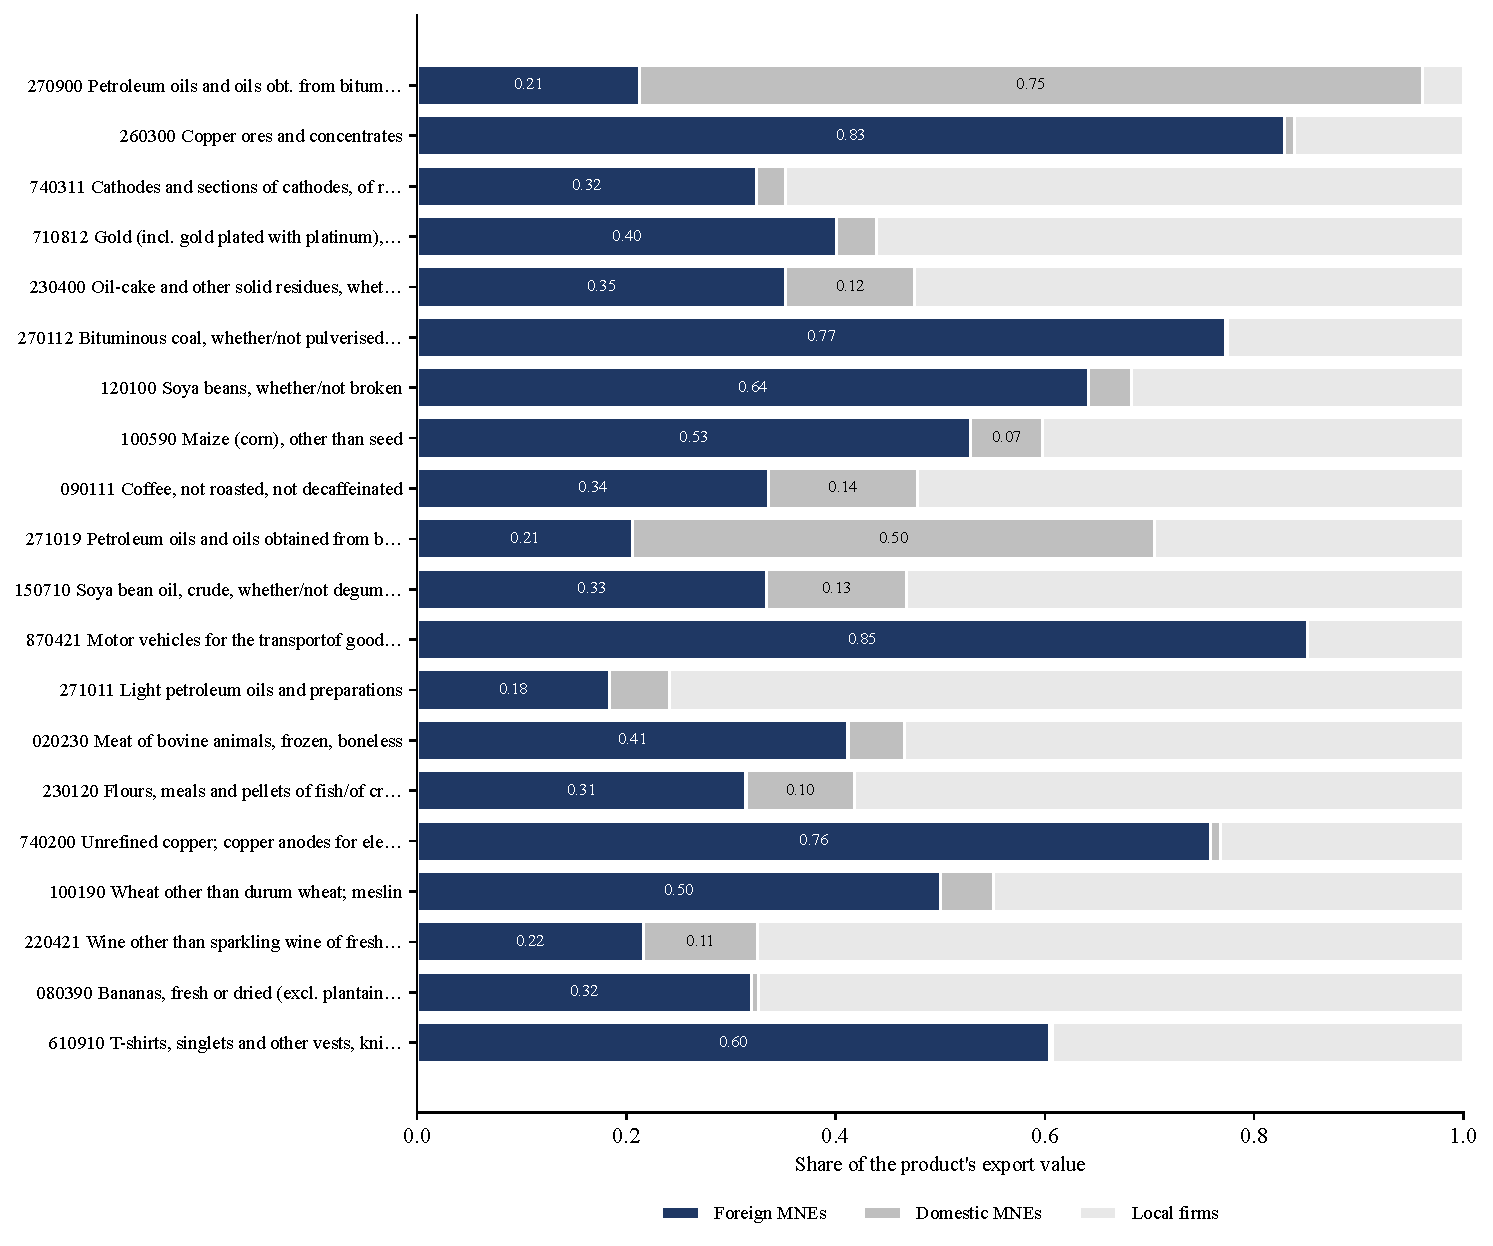
\includegraphics[width=1.0\textwidth,height=0.8\textheight,keepaspectratio]{figures/all/fig_wp1f_top20_hs6_stacked.pdf}%
  \caption{Ownership of the Twenty Largest Export Products}%
  \label{fig:hs_st_all}%
  \par\vspace{2pt}%
  \parbox{0.92\textwidth}{\footnotesize %
  \textit{Notes:} Shares of each product's export value. Twenty largest HS6 products by export value.\\[3pt]%
  \textit{Source:} Authors' calculations based on customs data matched to Orbis and Dun \& Bradstreet.}%
  \end{figure}
% ---- Figure: Ownership of the Twenty Largest Export Products, by Parent Country
\begin{figure}[H]\centering%
  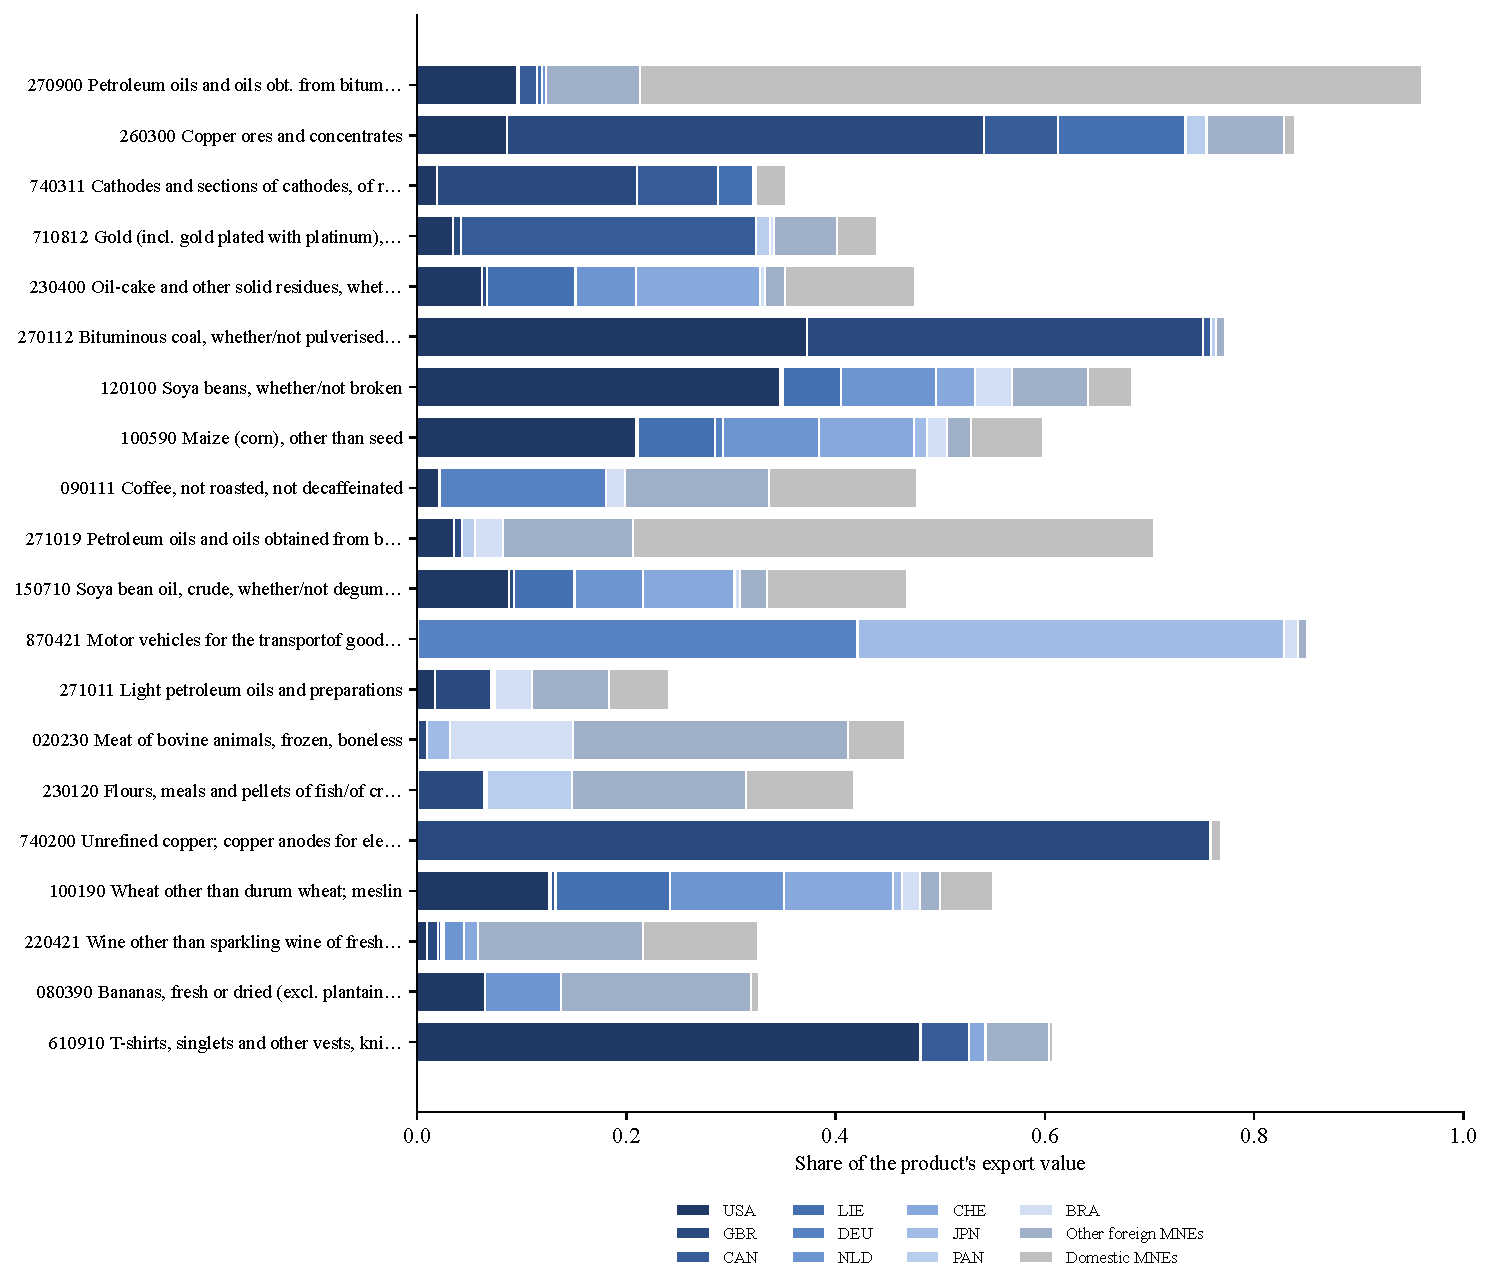
\includegraphics[width=1.0\textwidth,height=0.8\textheight,keepaspectratio]{figures/all/fig_wp1f_top20_hs6_by_parent.pdf}%
  \caption{Ownership of the Twenty Largest Export Products, by Parent Country}%
  \label{fig:hs_par_all}%
  \par\vspace{2pt}%
  \parbox{0.92\textwidth}{\footnotesize %
  \textit{Notes:} Shares of each product's export value. Foreign-MNE share split by country of the ultimate parent; the unfilled part of each bar is local firms.\\[3pt]%
  \textit{Source:} Authors' calculations based on customs data matched to Orbis and Dun \& Bradstreet.}%
  \end{figure}
% ---- Figure: Distribution of Export Value by Product-Level Foreign-Multinational Share
\begin{figure}[H]\centering%
  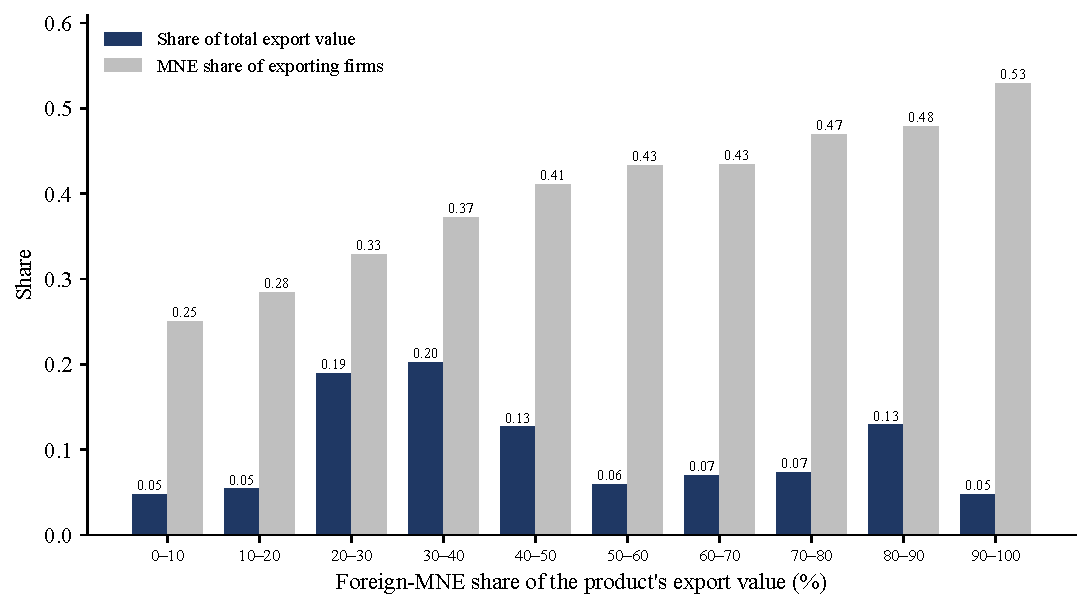
\includegraphics[width=0.85\textwidth,height=0.8\textheight,keepaspectratio]{figures/all/fig_wp1f_foreign_share_distribution.pdf}%
  \caption{Distribution of Export Value by Product-Level Foreign-Multinational Share}%
  \label{fig:hs_dist_all}%
  \par\vspace{2pt}%
  \parbox{0.92\textwidth}{\footnotesize %
  \textit{Notes:} Share of export value and MNE share of exporting firms, by the foreign-MNE share of each HS6 product's export value.\\[3pt]%
  \textit{Source:} Authors' calculations based on customs data matched to Orbis and Dun \& Bradstreet.}%
  \end{figure}
% ---- Table: Distribution of Export Value by Product-Level Foreign-Multinational Share
\begin{table}[H]\centering\small%
  \caption{Distribution of Export Value by Product-Level Foreign-Multinational Share}%
  \label{tab:hs_dist_t_all}%
  \adjustbox{max width=\textwidth, max totalheight=0.8\textheight}{\begin{tabular}{lrrr}
\toprule
Foreign share bin (\%) & Share of value & MNE share of exporting firms & HS6 products \\
\midrule
0--10 & 0.048 & 0.250 & 1,426 \\
10--20 & 0.054 & 0.285 & 731 \\
20--30 & 0.189 & 0.329 & 652 \\
30--40 & 0.202 & 0.372 & 591 \\
40--50 & 0.127 & 0.411 & 519 \\
50--60 & 0.059 & 0.433 & 442 \\
60--70 & 0.070 & 0.435 & 386 \\
70--80 & 0.074 & 0.470 & 311 \\
80--90 & 0.129 & 0.479 & 311 \\
90--100 & 0.048 & 0.530 & 560 \\
\bottomrule
\end{tabular}
}%
  \par\vspace{3pt}%
  \begin{minipage}{0.95\textwidth}\footnotesize %
  \textit{Notes:} Share of export value and MNE share of exporting firms, by the foreign-MNE share of each HS6 product's export value. MNE share of exporting firms: MNE firm--destination--product--year observations over all observations in the bin.\\[3pt]%
  \textit{Source:} Authors' calculations based on customs data matched to Orbis and Dun \& Bradstreet.%
  \end{minipage}%
  \end{table}
% ---- Figure: Concentration of Exports across Products
\begin{figure}[H]\centering%
  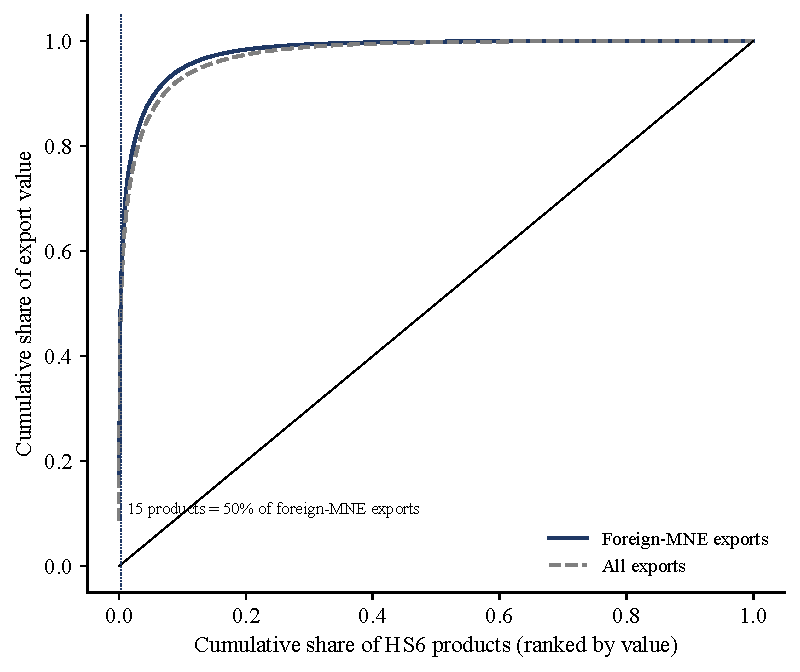
\includegraphics[width=0.6\textwidth,height=0.8\textheight,keepaspectratio]{figures/all/fig_wp1f_lorenz_foreign.pdf}%
  \caption{Concentration of Exports across Products}%
  \label{fig:hs_lor_all}%
  \par\vspace{2pt}%
  \parbox{0.92\textwidth}{\footnotesize %
  \textit{Notes:} Cumulative share of export value against the cumulative share of HS6 products, ranked by value, for foreign-MNE exports and for all exports.\\[3pt]%
  \textit{Source:} Authors' calculations based on customs data matched to Orbis and Dun \& Bradstreet.}%
  \end{figure}
% ---- Table: Exports and Multinational Shares, by HS Section
\begin{table}[H]\centering\footnotesize%
  \caption{Exports and Multinational Shares, by HS Section}%
  \label{tab:hs_sec_all}%
  \adjustbox{max width=\textwidth, max totalheight=0.8\textheight}{\begin{tabular}{@{}p{7.2cm} r r r r l@{}}
\toprule
HS section & US\$bn/yr & Foreign (\%) & Domestic (\%) & Local (\%) & Leading parent \\
\midrule
V Mineral products & 57.1 & 51 & 29 & 19 & GBR (0.42) \\
II Vegetable products & 33.5 & 42 & 7 & 51 & USA (0.33) \\
IV Prepared foodstuffs, beverages, tobacco & 25.9 & 37 & 10 & 53 & USA (0.21) \\
XV Base metals & 19.6 & 41 & 3 & 56 & GBR (0.44) \\
XIV Precious metals and stones & 15.3 & 41 & 4 & 56 & CAN (0.65) \\
I Live animals; animal products & 12.5 & 34 & 14 & 51 & SAU (0.19) \\
VI Chemicals & 11.6 & 49 & 14 & 37 & USA (0.25) \\
XVII Transport equipment & 9.7 & 78 & 4 & 18 & DEU (0.30) \\
XI Textiles and apparel & 6.9 & 49 & 3 & 48 & USA (0.62) \\
III Fats and oils & 6.9 & 31 & 10 & 59 & CHE (0.26) \\
XVI Machinery and electrical equipment & 6.2 & 63 & 4 & 33 & USA (0.41) \\
VII Plastics and rubber & 5.8 & 51 & 8 & 42 & USA (0.34) \\
X Pulp, paper & 3.4 & 54 & 28 & 18 & PAN (0.54) \\
XVIII Optical, precision instruments & 3.4 & 72 & 8 & 19 & USA (0.66) \\
IX Wood and articles & 1.9 & 27 & 34 & 39 & BHS (0.24) \\
VIII Hides, skins, leather & 1.6 & 40 & 12 & 49 & BGR (0.19) \\
XIII Stone, ceramics, glass & 0.9 & 49 & 4 & 46 & USA (0.32) \\
XX Miscellaneous manufactures & 0.9 & 53 & 7 & 40 & USA (0.48) \\
Unclassified & 0.5 & 49 & 29 & 23 & USA (0.39) \\
XII Footwear, headgear & 0.5 & 48 & 1 & 50 & USA (0.66) \\
XXI Works of art & 0.1 & 58 & 1 & 41 & BGR (0.94) \\
XIX Arms & 0.0 & 1 & 0 & 99 & CHE (0.82) \\
Special / unclassified (98-99) & 0.0 & 13 & 1 & 87 & USA (0.57) \\
\midrule
All sections & 224.5 & 46 & 14 & 40 & \\
\bottomrule
\end{tabular}
}%
  \par\vspace{3pt}%
  \begin{minipage}{0.95\textwidth}\footnotesize %
  \textit{Notes:} Foreign, domestic and local: percent of each section's export value. Leading parent: largest parent country and its share of the section's foreign-MNE exports. Values are annual averages in US\$ billion.\\[3pt]%
  \textit{Source:} Authors' calculations based on customs data matched to Orbis and Dun \& Bradstreet.%
  \end{minipage}%
  \end{table}
% ---- Table: Thirty Largest Export Products
\begin{table}[H]\centering\footnotesize%
  \caption{Thirty Largest Export Products}%
  \label{tab:hs_by_value_all}%
  \adjustbox{max width=\textwidth, max totalheight=0.8\textheight}{\begin{tabular}{@{}l p{6.4cm} r r r r l@{}}
\toprule
HS6 & Description & US\$bn/yr & Foreign (\%) & Domestic (\%) & Local (\%) & Leading parent \\
\midrule
270900 & Petroleum oils and oils obt. from bituminous mins., crude & 17.9 & 21 & 75 & 4 & USA (0.45) \\
260300 & Copper ores and concentrates & 17.6 & 83 & 1 & 16 & GBR (0.55) \\
740311 & Cathodes and sections of cathodes, of refined copper, unwrought & 10.4 & 32 & 3 & 65 & GBR (0.59) \\
710812 & Gold (incl. gold plated with platinum), in unwrought forms (excl. powder) & 13.4 & 40 & 4 & 56 & CAN (0.70) \\
230400 & Oil-cake and other solid residues, whether/\allowbreak{}not ground/\allowbreak{}in pellets, from extraction of soyabean ... & 10.8 & 35 & 12 & 52 & CHE (0.34) \\
270112 & Bituminous coal, whether/\allowbreak{}not pulverised but not agglomerated & 5.7 & 77 & 0 & 23 & GBR (0.49) \\
120100 & Soya beans, whether/\allowbreak{}not broken & 6.2 & 64 & 4 & 32 & USA (0.54) \\
100590 & Maize (corn), other than seed & 4.8 & 53 & 7 & 40 & USA (0.40) \\
090111 & Coffee, not roasted, not decaffeinated & 3.7 & 34 & 14 & 52 & DEU (0.47) \\
271019 & Petroleum oils and oils obtained from bituminous minerals (other than crude) and preparations ... & 3.6 & 21 & 50 & 30 & ESP (0.52) \\
150710 & Soya bean oil, crude, whether/\allowbreak{}not degummed, not chemically modified & 4.3 & 33 & 13 & 53 & USA (0.26) \\
870421 & Motor vehicles for the transportof goods (excl. of 8704.10), with C-I internal combustion pist... & 3.2 & 85 & 0 & 15 & DEU (0.49) \\
271011 & Light petroleum oils and preparations & 2.2 & 18 & 6 & 76 & GBR (0.29) \\
020230 & Meat of bovine animals, frozen, boneless & 2.1 & 41 & 5 & 53 & SAU (0.53) \\
230120 & Flours, meals and pellets of fish/\allowbreak{}of crustaceans, molluscs/\allowbreak{}other aquatic invertebrates & 1.7 & 31 & 10 & 58 & BMU (0.38) \\
740200 & Unrefined copper; copper anodes for electrolytic refining & 1.3 & 76 & 1 & 23 & GBR (1.00) \\
100190 & Wheat other than durum wheat; meslin & 1.9 & 50 & 5 & 45 & USA (0.25) \\
220421 & Wine other than sparkling wine of fresh grapes, incl. fortified; grape must with fermentation ... & 1.4 & 22 & 11 & 67 & FRA (0.25) \\
080390 & Bananas, fresh or dried (excl. plantains) [HS2012 code] & 1.4 & 32 & 1 & 67 & JOR (0.38) \\
610910 & T-shirts, singlets and other vests, knitted/\allowbreak{}crocheted, of cotton & 1.3 & 60 & 0 & 39 & USA (0.79) \\
260800 & Zinc ores and concentrates & 1.5 & 72 & 0 & 27 & GBR (0.67) \\
080610 & Grapes, fresh & 1.1 & 29 & 9 & 62 & ESP (0.29) \\
260111 & Iron ores and concentrates (excl. roasted iron pyrites), non-agglomerated & 1.1 & 2 & 47 & 51 & CAN (0.65) \\
260700 & Lead ores and concentrates & 1.3 & 58 & 0 & 42 & GBR (0.69) \\
870323 & Vehicles (excl. of 87.02 and 8703.10) principally designed for the transportof persons, with s... & 1.3 & 75 & 0 & 25 & FRA (0.45) \\
020130 & Meat of bovine animals, fresh/\allowbreak{}chilled, boneless & 1.4 & 35 & 11 & 55 & SAU (0.63) \\
901890 & Instruments and appliances used in medical/\allowbreak{}surgical/\allowbreak{}veterinary sciences, incl. other electro-m... & 1.4 & 89 & 0 & 11 & USA (0.52) \\
300490 & Medicaments (excluding goods of heading 30.02/\allowbreak{}30.05/\allowbreak{}30.06/\allowbreak{}3004.10-3004.50) consisting of mixed... & 1.0 & 55 & 7 & 38 & USA (0.29) \\
382490 & Chemical productsandpreparations of the chemical/\allowbreak{}allied industries (including those consisting... & 1.2 & 36 & 14 & 50 & LIE (0.61) \\
470321 & Chemical wood pulp, soda/\allowbreak{}sulphate, other than dissolving grades, semi-bleached/\allowbreak{}bleached, conif... & 0.7 & 71 & 29 & 0 & PAN (0.82) \\
\bottomrule
\end{tabular}
}%
  \par\vspace{3pt}%
  \begin{minipage}{0.95\textwidth}\footnotesize %
  \textit{Notes:} Thirty largest HS6 products by export value. Foreign, domestic and local: percent of the product's export value. Leading parent: largest parent country and its share of the product's foreign-MNE exports. Values are annual averages in US\$ billion.\\[3pt]%
  \textit{Source:} Authors' calculations based on customs data matched to Orbis and Dun \& Bradstreet.%
  \end{minipage}%
  \end{table}
% ---- Table: Thirty Largest Export Products of Foreign Multinationals
\begin{table}[H]\centering\footnotesize%
  \caption{Thirty Largest Export Products of Foreign Multinationals}%
  \label{tab:hs_by_foreign_value_all}%
  \adjustbox{max width=\textwidth, max totalheight=0.8\textheight}{\begin{tabular}{@{}l p{6.4cm} r r r r l@{}}
\toprule
HS6 & Description & US\$bn/yr & Foreign (\%) & Domestic (\%) & Local (\%) & Leading parent \\
\midrule
260300 & Copper ores and concentrates & 17.6 & 83 & 1 & 16 & GBR (0.55) \\
710812 & Gold (incl. gold plated with platinum), in unwrought forms (excl. powder) & 13.4 & 40 & 4 & 56 & CAN (0.70) \\
270112 & Bituminous coal, whether/\allowbreak{}not pulverised but not agglomerated & 5.7 & 77 & 0 & 23 & GBR (0.49) \\
740311 & Cathodes and sections of cathodes, of refined copper, unwrought & 10.4 & 32 & 3 & 65 & GBR (0.59) \\
270900 & Petroleum oils and oils obt. from bituminous mins., crude & 17.9 & 21 & 75 & 4 & USA (0.45) \\
120100 & Soya beans, whether/\allowbreak{}not broken & 6.2 & 64 & 4 & 32 & USA (0.54) \\
230400 & Oil-cake and other solid residues, whether/\allowbreak{}not ground/\allowbreak{}in pellets, from extraction of soyabean ... & 10.8 & 35 & 12 & 52 & CHE (0.34) \\
870421 & Motor vehicles for the transportof goods (excl. of 8704.10), with C-I internal combustion pist... & 3.2 & 85 & 0 & 15 & DEU (0.49) \\
100590 & Maize (corn), other than seed & 4.8 & 53 & 7 & 40 & USA (0.40) \\
090111 & Coffee, not roasted, not decaffeinated & 3.7 & 34 & 14 & 52 & DEU (0.47) \\
740200 & Unrefined copper; copper anodes for electrolytic refining & 1.3 & 76 & 1 & 23 & GBR (1.00) \\
150710 & Soya bean oil, crude, whether/\allowbreak{}not degummed, not chemically modified & 4.3 & 33 & 13 & 53 & USA (0.26) \\
901890 & Instruments and appliances used in medical/\allowbreak{}surgical/\allowbreak{}veterinary sciences, incl. other electro-m... & 1.4 & 89 & 0 & 11 & USA (0.52) \\
260800 & Zinc ores and concentrates & 1.5 & 72 & 0 & 27 & GBR (0.67) \\
870323 & Vehicles (excl. of 87.02 and 8703.10) principally designed for the transportof persons, with s... & 1.3 & 75 & 0 & 25 & FRA (0.45) \\
610910 & T-shirts, singlets and other vests, knitted/\allowbreak{}crocheted, of cotton & 1.3 & 60 & 0 & 39 & USA (0.79) \\
271111 & Natural gas, liquefied & 0.9 & 100 & 0 & 0 & USA (1.00) \\
100190 & Wheat other than durum wheat; meslin & 1.9 & 50 & 5 & 45 & USA (0.25) \\
720260 & Ferro-nickel, in granular/\allowbreak{}powder form & 0.8 & 100 & 0 & 0 & ZAF (0.85) \\
271019 & Petroleum oils and oils obtained from bituminous minerals (other than crude) and preparations ... & 3.6 & 21 & 50 & 30 & ESP (0.52) \\
020230 & Meat of bovine animals, frozen, boneless & 2.1 & 41 & 5 & 53 & SAU (0.53) \\
901839 & Catheters, cannulae and the like & 0.9 & 89 & 0 & 11 & USA (0.96) \\
854231 & Electronic integrated  circuits, processors and controllers, whether/\allowbreak{}not combined with memorie... & 0.8 & 99 & 0 & 1 & USA (0.98) \\
260700 & Lead ores and concentrates & 1.3 & 58 & 0 & 42 & GBR (0.69) \\
870322 & Vehicles (excl. of 87.02 and 8703.10) principally designed for the transportof persons, with s... & 0.8 & 100 & 0 & 0 & USA (0.59) \\
470321 & Chemical wood pulp, soda/\allowbreak{}sulphate, other than dissolving grades, semi-bleached/\allowbreak{}bleached, conif... & 0.7 & 71 & 29 & 0 & PAN (0.82) \\
210690 & Food preparations, n.e.s. & 0.7 & 81 & 1 & 18 & USA (0.79) \\
300490 & Medicaments (excluding goods of heading 30.02/\allowbreak{}30.05/\allowbreak{}30.06/\allowbreak{}3004.10-3004.50) consisting of mixed... & 1.0 & 55 & 7 & 38 & USA (0.29) \\
870840 & Gear boxes and parts thereof, of the motor vehicles of headings 87.01 to 87.05. & 0.6 & 99 & 0 & 1 & DEU (0.74) \\
261610 & Silver ores and concentrates & 0.8 & 76 & 0 & 24 & GBR (0.47) \\
\bottomrule
\end{tabular}
}%
  \par\vspace{3pt}%
  \begin{minipage}{0.95\textwidth}\footnotesize %
  \textit{Notes:} Thirty largest HS6 products by foreign-MNE export value. Foreign, domestic and local: percent of the product's export value. Leading parent: largest parent country and its share of the product's foreign-MNE exports. Values are annual averages in US\$ billion.\\[3pt]%
  \textit{Source:} Authors' calculations based on customs data matched to Orbis and Dun \& Bradstreet.%
  \end{minipage}%
  \end{table}
% ---- Table: Products with the Highest Foreign-Multinational Share
\begin{table}[H]\centering\footnotesize%
  \caption{Products with the Highest Foreign-Multinational Share}%
  \label{tab:hs_by_foreign_share_all}%
  \adjustbox{max width=\textwidth, max totalheight=0.8\textheight}{\begin{tabular}{@{}l p{6.4cm} r r r r l@{}}
\toprule
HS6 & Description & US\$bn/yr & Foreign (\%) & Domestic (\%) & Local (\%) & Leading parent \\
\midrule
720260 & Ferro-nickel, in granular/\allowbreak{}powder form & 0.76 & 100 & 0 & 0 & ZAF (0.85) \\
790500 & Zinc plates, sheets, strip and foil & 0.05 & 100 & 0 & 0 & GBR (0.94) \\
790112 & Zinc, not alloyed, unwrought, containing by weight <99.99\% of zinc & 0.22 & 100 & 0 & 0 & BRA (1.00) \\
870321 & Vehicles (excl. of 87.02 and 8703.10) principally designed for the transportof persons, with s... & 0.53 & 100 & 0 & 0 & NLD (0.49) \\
390410 & Poly(vinyl chloride), not mixed with any other substance, in primary forms & 0.38 & 100 & 0 & 0 & MEX (0.83) \\
271111 & Natural gas, liquefied & 0.85 & 100 & 0 & 0 & USA (1.00) \\
870322 & Vehicles (excl. of 87.02 and 8703.10) principally designed for the transportof persons, with s... & 0.82 & 100 & 0 & 0 & USA (0.59) \\
870333 & Vehicles principally designed for the transportof persons (excl. of 87.02 and 8703.10-8703.24)... & 0.39 & 100 & 0 & 0 & JPN (1.00) \\
251010 & Natural calcium phosphates, natural aluminium calcium phosphates and phosphatic chalk, unground & 0.28 & 100 & 0 & 0 & BRA (1.00) \\
280300 & Carbon (carbon blacks and other forms of carbon, n.e.s.) & 0.08 & 100 & 0 & 0 & USA (0.99) \\
470311 & Chemical wood pulp, soda/\allowbreak{}sulphate, other than dissolving grades, unbleached, coniferous & 0.14 & 100 & 0 & 0 & PAN (1.00) \\
300691 & Appliances identifiable for ostomy use & 0.19 & 100 & 0 & 0 & GBR (0.80) \\
853620 & Automatic circuit breakers, for a voltage not >1000V & 0.45 & 99 & 0 & 1 & IRL (0.89) \\
854231 & Electronic integrated  circuits, processors and controllers, whether/\allowbreak{}not combined with memorie... & 0.76 & 99 & 0 & 1 & USA (0.98) \\
381512 & Supported catalysts, with precious metal/\allowbreak{}precious metal comps. as the active substance & 0.08 & 99 & 0 & 1 & GBR (0.80) \\
870840 & Gear boxes and parts thereof, of the motor vehicles of headings 87.01 to 87.05. & 0.63 & 99 & 0 & 1 & DEU (0.74) \\
620711 & Men's/\allowbreak{}boys' underpants and briefs (excl. knitted/\allowbreak{}crocheted), of cotton & 0.05 & 98 & 0 & 2 & USA (1.00) \\
854430 & Ignition wiring sets and other wiring sets of a kind used in vehicles/\allowbreak{}aircraft/\allowbreak{}ships & 0.23 & 98 & 0 & 2 & JPN (0.81) \\
740710 & Bars, rods and profiles, of refined copper & 0.06 & 98 & 0 & 1 & MEX (0.73) \\
390120 & Polyethylene having a sp.gr. of 0.94/\allowbreak{}more, in primary forms & 0.13 & 98 & 0 & 2 & USA (0.98) \\
961900 & Sanitary towels and tampons, napkins and napkin liners for babies and similar sanitary article... & 0.22 & 97 & 1 & 1 & USA (0.79) \\
350300 & Gelatin, incl. gelatin in rectangular (incl. square) sheets, whether/\allowbreak{}not surface-worked /\allowbreak{}colou... & 0.08 & 97 & 0 & 3 & BEL (0.43) \\
790111 & Zinc, not alloyed, unwrought, containing by weight 99.99\%/\allowbreak{}more of zinc & 0.35 & 97 & 0 & 3 & BRA (0.90) \\
521213 & Woven fabrics of cotton (excl. of 52.08-52.11), dyed, weighing not >200 g/\allowbreak{}m2 & 0.13 & 96 & 0 & 4 & USA (1.00) \\
390190 & Polymers of ethylene, in primary forms (excl. of 3901.10-3901.30) & 0.13 & 96 & 0 & 4 & USA (1.00) \\
840820 & Compression-ignition internal combustion piston engines (diesel/\allowbreak{}semi-diesel engines) of a kind... & 0.19 & 96 & 0 & 4 & USA (0.54) \\
761010 & Doors, windows and their frames and thresholds for doors, of aluminium & 0.13 & 96 & 0 & 4 & CYM (0.99) \\
870422 & Motor vehicles for the transportof goods (excl. of 8704.10), with C-I internal combustion pist... & 0.08 & 96 & 0 & 4 & JPN (0.88) \\
281700 & Zinc oxide; zinc peroxide & 0.07 & 95 & 0 & 5 & BRA (0.80) \\
300610 & Sterile surgical catgut, similar sterile suture materials (including sterile absorbable surgic... & 0.14 & 95 & 3 & 2 & IRL (0.98) \\
\bottomrule
\end{tabular}
}%
  \par\vspace{3pt}%
  \begin{minipage}{0.95\textwidth}\footnotesize %
  \textit{Notes:} HS6 products with exports of at least US\$500 million over the period, ranked by foreign-MNE share. Foreign, domestic and local: percent of the product's export value. Leading parent: largest parent country and its share of the product's foreign-MNE exports. Values are annual averages in US\$ billion.\\[3pt]%
  \textit{Source:} Authors' calculations based on customs data matched to Orbis and Dun \& Bradstreet.%
  \end{minipage}%
  \end{table}
% ---- Table: Products with the Highest Domestic-Multinational Share
\begin{table}[H]\centering\footnotesize%
  \caption{Products with the Highest Domestic-Multinational Share}%
  \label{tab:hs_by_domestic_share_all}%
  \adjustbox{max width=\textwidth, max totalheight=0.8\textheight}{\begin{tabular}{@{}l p{6.4cm} r r r r l@{}}
\toprule
HS6 & Description & US\$bn/yr & Foreign (\%) & Domestic (\%) & Local (\%) & Leading parent \\
\midrule
282520 & Lithium oxide and hydroxide & 0.0 & 0 & 100 & 0 & -- \\
481092 & Paper and paperboard(excl. of 4810.13-4810.39), coated on one/\allowbreak{}both sides with kaolin (China cl... & 0.2 & 1 & 99 & 0 & IRL (0.84) \\
310420 & Potassium chloride & 0.1 & 3 & 95 & 2 & DZA (0.58) \\
441193 & Fibreboard of wood/\allowbreak{}other ligneous materials, whether/\allowbreak{}not bonded with resins/\allowbreak{}other organic subs... & 0.0 & 1 & 94 & 5 & ESP (0.94) \\
260112 & Iron ores and concentrates (excl. roasted iron pyrites), agglomerated & 0.1 & 7 & 88 & 4 & CHE (1.00) \\
350110 & Casein & 0.1 & 0 & 84 & 16 & CHL (0.80) \\
020727 & Cuts and edible offal of turkey, frozen & 0.0 & 1 & 82 & 17 & JPN (0.45) \\
730640 & Tubes, pipes and hollow profiles (excl. of 7306.10-7306.30), welded, of circular cross-section... & 0.1 & 15 & 82 & 3 & DEU (0.60) \\
270900 & Petroleum oils and oils obt. from bituminous mins., crude & 17.9 & 21 & 75 & 4 & USA (0.45) \\
390390 & Polymers of styrene, in primary forms (excl. of 3903.11-3903.30) & 0.0 & 15 & 73 & 12 & NLD (0.78) \\
440711 & Wood sawn/\allowbreak{}chipped length wise, sliced/\allowbreak{}peeled, whether/\allowbreak{}not planed, sanded/\allowbreak{}end-jointed, of a thi... & 0.2 & 10 & 71 & 19 & BHS (0.67) \\
441239 & Plywood, consisting solely of sheets of wood (other than bamboo,excl. of 4412.31 and4412.32), ... & 0.2 & 28 & 71 & 1 & VGB (0.46) \\
390319 & Polystyrene other than expansible, in primary forms & 0.1 & 22 & 67 & 11 & PAN (0.99) \\
040610 & Fresh (unripened/\allowbreak{}uncured) cheese, incl. whey cheese, and curd & 0.1 & 12 & 66 & 22 & MUS (0.36) \\
283691 & Lithium carbonates & 0.6 & 14 & 65 & 21 & USA (0.54) \\
540219 & High tenacity yarn other than textured yarn/\allowbreak{}sewing thread, of nylon/\allowbreak{}other polyamides (excl. of... & 0.1 & 36 & 64 & 0 & GBR (0.80) \\
481141 & Gummed/\allowbreak{}adhesive paper,paperboard,coated, impregnated, covered, surface-coloured, surface-decor... & 0.1 & 26 & 62 & 12 & GBR (0.56) \\
902139 & Artificial parts of the body other than teeth, dental fittings and joints & 0.4 & 10 & 60 & 30 & VGB (0.46) \\
722830 & Bars and rods of other alloy steel (excl. of 72.27, 7228.10 and 7228.20), not further worked t... & 0.1 & 25 & 56 & 19 & SGP (0.59) \\
020329 & Meat of swine (excl. carcasses/\allowbreak{}half-carcasses/\allowbreak{}hams/\allowbreak{}shoulders and cuts thereof ), froxen & 0.2 & 29 & 54 & 17 & JPN (1.00) \\
470329 & Chemical wood pulp, soda/\allowbreak{}sulphate, other than dissolving grades, semi-bleached/\allowbreak{}bleached, non-c... & 0.6 & 46 & 54 & 0 & PAN (1.00) \\
491110 & Trade advertising material, commercial cataloguesandthe like & 0.1 & 16 & 53 & 31 & USA (0.45) \\
880240 & Aeroplanes and other aircraft, of an unladen weight >15000kg & 0.6 & 40 & 53 & 7 & CHL (0.99) \\
410449 & Tanned/\allowbreak{}crust hides and skins of bovine (incl. buffalo)/\allowbreak{}equine animals, without hair on, in the... & 0.1 & 37 & 52 & 12 & URY (0.71) \\
271019 & Petroleum oils and oils obtained from bituminous minerals (other than crude) and preparations ... & 3.6 & 21 & 50 & 30 & ESP (0.52) \\
210111 & Extracts, essences and concentrates of coffee & 0.2 & 23 & 48 & 29 & CHE (0.70) \\
260111 & Iron ores and concentrates (excl. roasted iron pyrites), non-agglomerated & 1.1 & 2 & 47 & 51 & CAN (0.65) \\
330300 & Perfumes and toilet waters & 0.1 & 34 & 46 & 20 & PAN (0.38) \\
030319 & Pacific salmon (Oncorhynchus gorbuscha/\allowbreak{}keta/\allowbreak{}tschawytscha/\allowbreak{}kisutch/\allowbreak{}masou/\allowbreak{}rhodurus), frozen (excl... & 0.1 & 8 & 44 & 47 & CAN (0.39) \\
391990 & Self-adhesive plates, sheets, film, foil, tape, strip and other flat shapes, of plastics, whet... & 0.1 & 41 & 44 & 15 & GBR (0.57) \\
\bottomrule
\end{tabular}
}%
  \par\vspace{3pt}%
  \begin{minipage}{0.95\textwidth}\footnotesize %
  \textit{Notes:} HS6 products with exports of at least US\$500 million over the period, ranked by domestic-MNE share. Foreign, domestic and local: percent of the product's export value. Leading parent: largest parent country and its share of the product's foreign-MNE exports. Values are annual averages in US\$ billion.\\[3pt]%
  \textit{Source:} Authors' calculations based on customs data matched to Orbis and Dun \& Bradstreet.%
  \end{minipage}%
  \end{table}

\section{Sectors}\label{sec:sectors}
% ---- Table: Exports and Multinational Shares, by Sector
\begin{table}[H]\centering\small%
  \caption{Exports and Multinational Shares, by Sector}%
  \label{tab:four}%
  \adjustbox{max width=\textwidth, max totalheight=0.8\textheight}{\begin{tabular}{@{}l r r r r l@{}}
\toprule
Sector & Total exports (US\$bn/yr) & MNE exports (US\$bn/yr) & Foreign (\%) & Domestic (\%) & Leading parents (share of foreign) \\
\midrule
Agriculture & 78.9 & 37.8 & 38.1 & 9.5 & USA 0.24, CHE 0.11, NLD 0.10 \\
Mining \& fuels & 72.4 & 52.4 & 49.2 & 24.5 & GBR 0.36, USA 0.21, CAN 0.16 \\
Manufacturing & 72.7 & 43.9 & 51.6 & 8.0 & USA 0.25, GBR 0.14, DEU 0.09 \\
Rest & 0.5 & 0.4 & 47.9 & 28.0 & USA 0.39, GBR 0.12, ESP 0.11 \\
\midrule
All & 224.5 & 134.5 & 46.3 & 14.1 & \\
\bottomrule
\end{tabular}
}%
  \par\vspace{3pt}%
  \begin{minipage}{0.95\textwidth}\footnotesize %
  \textit{Notes:} Foreign and domestic: percent of the sector's export value. Other goods: HS 98--99 and unclassified codes. Leading parents: the three largest parent countries and their share of the row's foreign-MNE exports. Values are annual averages in US\$ billion.\\[3pt]%
  \textit{Source:} Authors' calculations based on customs data matched to Orbis and Dun \& Bradstreet.%
  \end{minipage}%
  \end{table}
% ---- Figure: Multinational Share of Export Value, by Sector
\begin{figure}[H]\centering%
  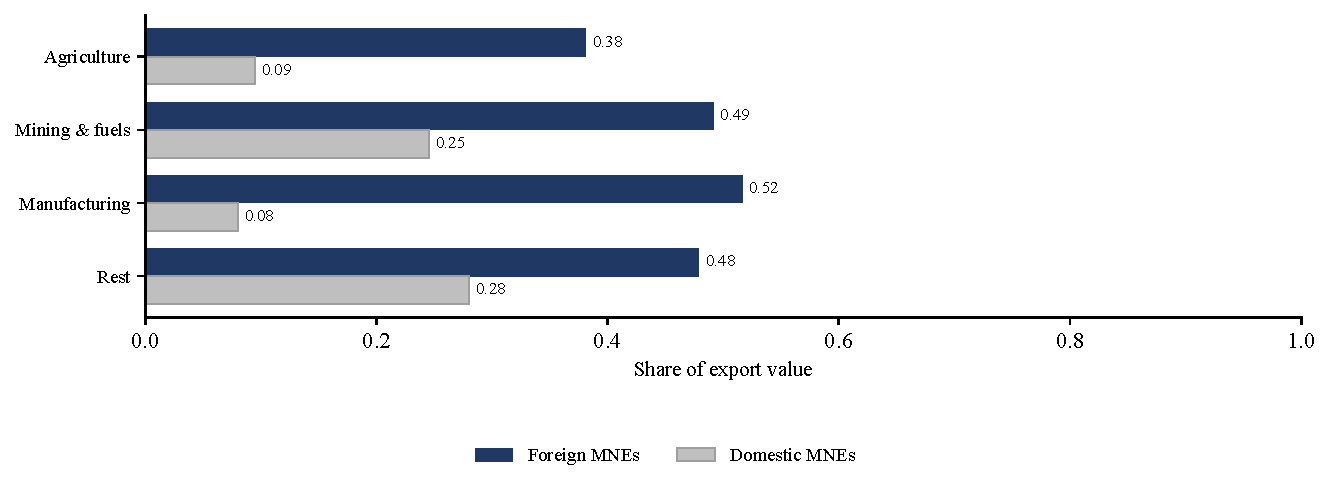
\includegraphics[width=0.8\textwidth,height=0.8\textheight,keepaspectratio]{figures/sectors/fig_wp2_four_sectors.pdf}%
  \caption{Multinational Share of Export Value, by Sector}%
  \label{fig:four_f}%
  \par\vspace{2pt}%
  \parbox{0.92\textwidth}{\footnotesize %
  \textit{Notes:} Shares of export value, all available years pooled. Agriculture: HS 01--24. Mining and fuels: HS 25--27 and 71. Manufacturing: HS 28--97 excluding 71.\\[3pt]%
  \textit{Source:} Authors' calculations based on customs data matched to Orbis and Dun \& Bradstreet.}%
  \end{figure}
% ---- Figure: Foreign-Multinational Share of Export Value, by Exporting Country and Sector
\begin{figure}[H]\centering%
  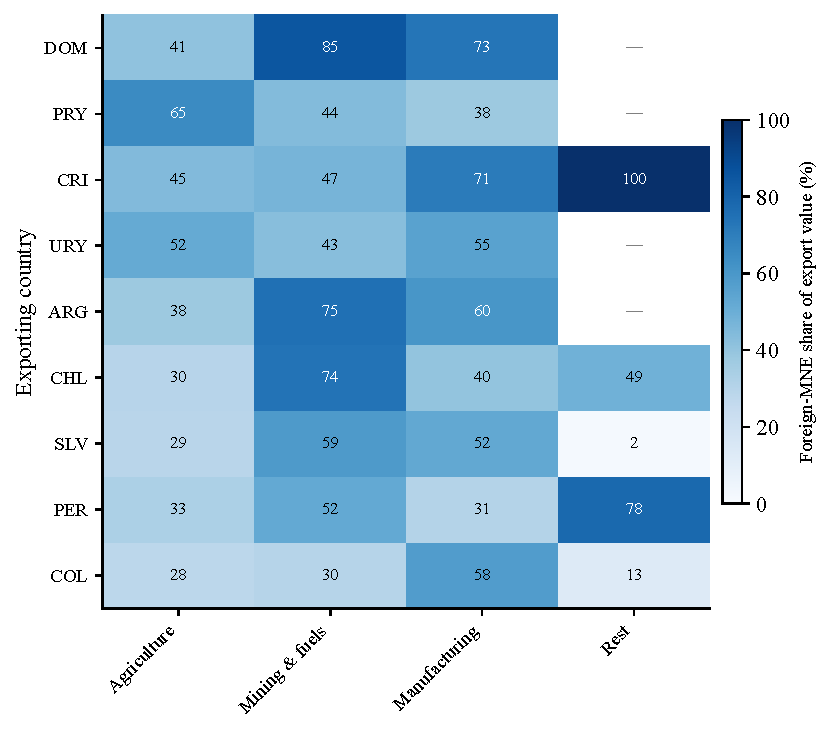
\includegraphics[width=0.8\textwidth,height=0.8\textheight,keepaspectratio]{figures/sectors/fig_wp2_origin_x_sector.pdf}%
  \caption{Foreign-Multinational Share of Export Value, by Exporting Country and Sector}%
  \label{fig:ox_f}%
  \par\vspace{2pt}%
  \parbox{0.92\textwidth}{\footnotesize %
  \textit{Notes:} Percent of each country's export value in each sector shipped by foreign MNEs.\\[3pt]%
  \textit{Source:} Authors' calculations based on customs data matched to Orbis and Dun \& Bradstreet.}%
  \end{figure}
% ---- Table: Exports by Exporting Country and Sector
\begin{table}[H]\centering\small%
  \caption{Exports by Exporting Country and Sector}%
  \label{tab:ox_t}%
  \adjustbox{max width=\textwidth, max totalheight=0.8\textheight}{\begin{tabular}{lrrrrr}
\toprule
Origin & Agriculture & Mining \& fuels & Manufacturing & Rest & All \\
\midrule
\multicolumn{6}{l}{\textit{Panel A: composition of the origin's exports, \% (rows sum to 100)}} \\
ARG & 57.4 & 9.9 & 32.7 & 0.0 & 100.0 \\
CHL & 21.9 & 29.7 & 46.9 & 1.4 & 100.0 \\
COL & 16.3 & 63.4 & 20.3 & 0.0 & 100.0 \\
CRI & 41.5 & 1.0 & 57.5 & 0.0 & 100.0 \\
DOM & 23.1 & 22.8 & 54.1 & 0.0 & 100.0 \\
PER & 19.4 & 61.0 & 19.6 & 0.0 & 100.0 \\
PRY & 85.2 & 1.1 & 13.7 & 0.0 & 100.0 \\
SLV & 22.1 & 3.0 & 74.9 & 0.0 & 100.0 \\
URY & 63.0 & 2.4 & 34.6 & 0.0 & 100.0 \\
All origins & 32.9 & 33.9 & 32.9 & 0.3 & 100.0 \\
\midrule
\multicolumn{6}{l}{\textit{Panel B: foreign-MNE share of export value, \%}} \\
ARG & 37.8 & 75.1 & 60.4 & -- & 48.9 \\
CHL & 29.6 & 73.9 & 39.9 & 48.6 & 47.9 \\
COL & 28.0 & 30.1 & 57.8 & 12.7 & 35.3 \\
CRI & 44.5 & 46.9 & 70.9 & 100.0 & 59.7 \\
DOM & 40.7 & 85.3 & 73.2 & -- & 68.4 \\
PER & 33.0 & 52.2 & 30.6 & 78.0 & 44.2 \\
PRY & 65.0 & 44.1 & 37.9 & -- & 61.1 \\
SLV & 28.9 & 58.8 & 52.5 & 1.5 & 47.4 \\
URY & 51.8 & 42.9 & 55.3 & -- & 52.8 \\
All origins & 38.1 & 49.2 & 51.6 & 47.9 & 46.3 \\
\bottomrule
\end{tabular}
}%
  \par\vspace{3pt}%
  \begin{minipage}{0.95\textwidth}\footnotesize %
  \textit{Notes:} Panel A: composition of each country's exports by sector (rows add to 100). Panel B: percent of each cell's export value shipped by foreign MNEs.\\[3pt]%
  \textit{Source:} Authors' calculations based on customs data matched to Orbis and Dun \& Bradstreet.%
  \end{minipage}%
  \end{table}
% ---- Table: Industry of Matched Exporting Affiliates
\begin{table}[H]\centering\small%
  \caption{Industry of Matched Exporting Affiliates}%
  \label{tab:services}%
  \adjustbox{max width=\textwidth, max totalheight=0.8\textheight}{\begin{tabular}{lr}
\toprule
NAICS sector of the matched exporting affiliate & \% of matched export value \\
\midrule
goods-producing or unknown & 82.4 \\
information, finance, professional, holdings (51--56) & 7.7 \\
wholesale / retail trade (42--45) & 7.4 \\
other services (61--92) & 1.8 \\
transport, logistics (48--49) & 0.6 \\
\bottomrule
\end{tabular}
}%
  \par\vspace{3pt}%
  \begin{minipage}{0.95\textwidth}\footnotesize %
  \textit{Notes:} Percent of matched export value, by NAICS sector of the exporting affiliate. Services are not observed in customs records; the table shows how much of goods exports is shipped by affiliates classified in service industries.\\[3pt]%
  \textit{Source:} Authors' calculations based on customs data matched to Orbis and Dun \& Bradstreet.%
  \end{minipage}%
  \end{table}
% ---- Table: Foreign-Multinational Exports by Sector and Destination Region
\begin{table}[H]\centering\small%
  \caption{Foreign-Multinational Exports by Sector and Destination Region}%
  \label{tab:sdr}%
  \adjustbox{max width=\textwidth, max totalheight=0.8\textheight}{\begin{tabular}{lrrrrrrrr}
\toprule
Sector / Destination region & Latin America & North America & Europe & Asia & Africa & Oceania & Rest of World & Total \\
\midrule
Agriculture & 31.1 & 13.8 & 20.2 & 28.1 & 6.1 & 0.4 & 0.4 & 30.7 \\
Mining \& fuels & 14.3 & 14.6 & 24.7 & 45.5 & 0.5 & 0.2 & 0.2 & 36.0 \\
Manufacturing & 50.8 & 20.7 & 9.3 & 17.3 & 0.7 & 1.1 & 0.2 & 38.5 \\
Rest & 37.3 & 42.2 & 17.2 & 2.9 & 0.1 & 0.2 & 0.1 & 0.2 \\
\bottomrule
\end{tabular}
}%
  \par\vspace{3pt}%
  \begin{minipage}{0.95\textwidth}\footnotesize %
  \textit{Notes:} Percent of each sector's foreign-MNE exports, by destination region (rows add to 100). Last column: foreign-MNE exports. Values are annual averages in US\$ billion.\\[3pt]%
  \textit{Source:} Authors' calculations based on customs data matched to Orbis and Dun \& Bradstreet.%
  \end{minipage}%
  \end{table}
\end{document}
